\documentclass{article}

% NeurIPS 2025 formatting
%\usepackage{neurips_2025}
\usepackage[preprint]{neurips_2025} % Ensure this is the desired option (preprint, final, etc.)
\usepackage{natbib}
\bibliographystyle{plainnat} % Moved from end of doc to preamble for consistency

% Additional packages
\usepackage[utf8]{inputenc} % allow utf-8 input
\usepackage{fontenc}    % use 8-bit T1 fonts
\usepackage{hyperref}       % hyperlinks
\hypersetup{
    colorlinks=false,   % Don't color the links
    pdfborder={0 0 0},  % No border around links (set to 0)
    hidelinks           % Hide all visual cues of links
}
\usepackage{url}            % simple URL typesetting
\usepackage{booktabs}       % professional-quality tables
\usepackage{amsfonts}       % blackboard math symbols
\usepackage{nicefrac}       % compact symbols for 1/2, etc.
\usepackage{microtype}      % microtypography
\usepackage[usenames,dvipsnames]{xcolor}         % colors
\usepackage{amsmath,amssymb,amsthm}
\usepackage{enumitem}
\usepackage{geometry} % Consider adjusting margins if needed, or removing if default is fine
\usepackage{tikz}
\usepackage{graphicx}
\usetikzlibrary{arrows.meta,positioning,fit,backgrounds,calc}
\graphicspath{{./POC/figures/}{./paper/images/}{./figures/}} % Added POC and figures to graphicspath

%%%% Macros
\newcommand{\Loss}{\mathcal{L}}
\newcommand{\R}{\mathbb{R}}
\newcommand{\E}{\mathbb{E}}
\newcommand{\He}{\mathrm{He}}
% Comments: 
% \newcommand{\giulia}[1]{{\color{ForestGreen}\textbf{Giulia:} #1}} % Keep for author's internal review if needed
%\newcommand{\giulia}[1]{} % Uncomment to hide comments

\usepackage[textsize=tiny]{todonotes}
% \usepackage{colortbl}

% \newcommand{\mf}[1]{\todo[color=orange!30,size=\tiny]{MF: #1}}
% \newcommand{\keivan}[1]{\todo[color=blue!30,size=\tiny]{K1: #1}}
% \newcommand{\ff}[1]{\todo[color=blue!30,size=\tiny]{FF: #1}}
% \newcommand{\AJ}[1]{\todo[color=green!30,size=\tiny]{AJ: #1}}

%%%% Theorem environments
\newtheorem{definition}{Definition}[section]
\newtheorem{lemma}{Lemma}[section]
\newtheorem{proposition}{Proposition}[section]
\newtheorem{corollary}{Corollary}[section]
\newtheorem{remark}{Remark}[section]


\title{Barriers for Learning in an Evolving World: \\a Mathematical Understanding of Loss of Plasticity}

\author{%
  Amir Joudaki$^{1}$ \And
  Giulia Lanzillotta$^{1}$ \And
  Mohammad Samragh Razlighi$^{2}$ \And
  Iman Mirzadeh$^{2}$ \And
  Keivan Alizadeh$^{2}$ \And
  Thomas Hofmann$^{1}$ \And
  Mehrdad Farajtabar$^{2}$ \And
  Fartash Faghri$^{2}$ %\And
  %\vspace{-20pt}
  \\
  $^{1}$ETH Zürich \quad
  $^{2}$Apple \\
  \texttt{amir.joudaki@inf.ethz.ch},
  \texttt{\{fartash, farajtabar\}@apple.com}
  %\texttt{\{amir.joudaki, giulia.lanzillotta, thomas.hofmann\}@inf.ethz.ch} \\
  %\texttt{\{fartash, m\_samraghrazlighi, imirzadeh, kalizadehvahid, m\_farajtabar\}@apple.com}
}

\begin{document}
\maketitle

\begin{abstract}
    Standard deep learning models excel when trained on stationary datasets but often falter in non-stationary environments where continuous adaptation is crucial. This paradigm struggle is significantly due to the degradation of future learning capacity, a phenomenon termed loss of plasticity (LoP). This work undertakes a first-principles investigation into the mechanisms underlying LoP in gradient-based models. We propose a formal definition of LoP grounded in dynamical systems theory, identifying stable manifolds in the parameter space that act as traps for gradient trajectories. Our analysis details two specific mechanisms leading to such traps: frozen units arising from activation saturation and cloned-unit manifolds resulting from representational redundancy. Furthermore, we explore conditions under which architectural choices or targeted perturbations might prevent or mitigate this plasticity collapse. 
    A core finding of our theoretical framework is the revelation of a fundamental tension: properties widely considered beneficial for generalization in conventional, static learning regimes, often characterized by distinct training and deployment phases, such as the emergence of low-rank representations or inherent simplicity biases, appear to directly contribute to LoP in continual learning scenarios. 
    By mathematically characterizing these barriers, this work pinpoints critical representational properties that hinder continuous learning, providing a clear direction for developing truly adaptive artificial intelligence. 
    Our theoretical analysis is supported by numerical simulations and empirical observations on various neural network architectures.
\end{abstract}

\section{Introduction}

The extraordinary success of back-propagation in training deep neural networks often relies on two implicit, yet critical, assumptions. First, \emph{stationarity}: the data distribution encountered during training is assumed to be identical, or very similar, to the distribution faced during deployment, rendering post-training adaptation minimal or absent. Second, \emph{single random initialization}: diversity and exploration potential are primarily introduced through a single random initialization of network parameters, a resource that is progressively consumed by optimization and not replenished. These assumptions falter when an artificial agent must operate and learn continuously within an environment characterized by changing dynamics or evolving task distributions. This scenario, often termed continual or lifelong learning, presents a significant challenge known as the stability-plasticity dilemma \citep{abraham2005memory, chaudhry2018riemannian}: the system must be stable enough to retain previously acquired knowledge, yet plastic enough to integrate new information effectively.

Empirically, standard deep networks subjected to long sequences of tasks or slowly drifting data streams often exhibit a decline in their learning capability \citep{dohare2024loss, berariu2021plasticity, dohare2021continual, nikishin2022primacy, lyle2023understanding}. This phenomenon, termed loss of plasticity (LoP), is distinct from catastrophic forgetting \citep{mccloskey1989catastrophic, ratcliff1990connectionist, french1999catastrophic}, where new learning overwrites old knowledge. LoP specifically refers to the diminished ability to learn new information effectively over time. Common symptoms include exploding weight magnitudes \citep{nikishin2022primacy}, activation saturation, the emergence of ``dead'' ReLU units (whose upstream parameters cease to update) \citep{nair2010rectified, sokar2023dormant, dohare2021continual, lyle2022understanding}, a collapse in the effective rank of hidden layer representations indicating reduced feature diversity \citep{papyan2020prevalence, huh2022lowrank, kumar2020implicit, gulcehre2022empirical}, and redundancy or diminishing contributions from network components like attention heads or filters \citep{lyle2023understanding}. Many of these issues have been highlighted in recent studies focusing on LoP \citep{dohare2023maintaining, kumar2024regenerative, ash2020warmstarting}.

\citet{dohare2024loss} argue compellingly that such failures are intrinsically linked to the back-propagation algorithm itself. They posit that gradient descent, optimized for transient, single-task learning, relies heavily on the initial random state for exploration, a resource that is consumed and not replenished during prolonged training. Their work demonstrates that standard deep learning methods can lose plasticity until they perform comparably to linear networks, and suggests that maintaining plasticity requires mechanisms beyond pure gradient descent, such as continually injecting diversity via methods like their proposed continual backpropagation.

\paragraph{Goal of this paper.}
Motivated by observations about LoP, our paper revisits the dynamics of gradient descent and back-propagation through the lens of dynamical systems theory. We seek to answer the fundamental question:
\begin{quote}
\emph{What structural features inherent in gradient flow dynamics inevitably lead to LoP, and how might we design algorithms or architectures capable of perpetual adaptation?}
\end{quote}
The central proposition advanced in this work is that the tendency of gradient-based optimization to favor low-rank or ``simple'' representations lies at the heart of plasticity loss. While properties like low effective rank and simplicity bias are often associated with improved generalization in the standard two-phase learning paradigm \citep{huh2022lowrank, papyan2020prevalence, zhang2017understanding}, we argue that these very properties become detrimental in continual learning settings. By reducing the effective dimensionality of the network's feature space, they limit its capacity to adapt to novel information, thus contributing to the LoP observed by \citep{dohare2024loss} and others.

\section{Preliminaries: A Dynamical Systems Framework for Plasticity}
\label{sec:framework}

Let $\theta\in\Theta\subseteq\R^p$ represent the parameters of a neural network. We consider training on a stream of data $\{(x_i,y_i)\}_{i=1}^N$ using gradient descent or its stochastic variants. The objective is typically to minimize a loss $\sum_{i=1}^N \Loss(\hat{y}_\theta(x_i),y_i),$ which we can succinctly refer to as $\Loss(\theta)$. The learning dynamics can be idealized by the continuous-time gradient flow:
\begin{equation}
    \frac{d\theta(t)}{dt} \;=\; -\nabla_\theta\Loss\bigl(\theta(t)\bigr).
    \label{eq:grad_flow}
\end{equation}
This perspective allows us to analyze the trajectory of parameters $\theta(t)$ in the parameter space $\Theta$ as driven by the negative gradient in the loss landscape \citep{saxe2014exact}.

We introduce the concept of a Loss of Plasticity (LoP) manifold to formalize the idea of gradient trajectories becoming trapped in lower-dimensional subspaces, thereby restricting future learning capacity.

\begin{definition}[LoP Manifold]
\label{def:lop}
A manifold $\mathcal{M}\subset\Theta$ induces LoP if the gradient of the loss function is tangent to the manifold at every point on the manifold. That is, $\nabla_\theta\Loss(\theta)\in T_\theta\mathcal{M}$ for all $\theta\in\mathcal{M}$, where $T_\theta\mathcal{M}$ denotes the tangent space of $\mathcal{M}$ at $\theta$. This tangency condition ensures that once the gradient flow enters $\mathcal{M}$, it remains within $\mathcal{M}$ under the dynamics of Equation~\ref{eq:grad_flow}.
\end{definition}



The stability of such a manifold determines its persistence as a trap for the learning dynamics.
\begin{definition}[Stability of LoP Manifold]
\label{def:lop_stability}
Let $N_\theta\mathcal{M}$ be the normal space to $\mathcal{M}$ at $\theta$. The stability of an LoP manifold is characterized by the Hessian $\nabla_\theta^2\Loss(\theta)$ in directions normal to $\mathcal{M}$:
        \begin{align}
        &\text{Stable LoP:}\; &&\forall v\in N_\theta\mathcal{M}\setminus\{0\}: v^\top\nabla_\theta^2\Loss(\theta)v > 0; \label{eq:stable}\\
        &\text{Unstable LoP:}\; &&\forall v\in N_\theta\mathcal{M}\setminus\{0\}: v^\top\nabla_\theta^2\Loss(\theta)v < 0; \label{eq:unstable}\\
        &\text{Saddle LoP:}\; &&\exists v_1,v_2\in N_\theta\mathcal{M}:\; v_1^\top\nabla_\theta^2\Loss v_1>0,\; v_2^\top\nabla_\theta^2\Loss v_2<0. \label{eq:saddle}
        \end{align}
\end{definition}

As we will elaborate later, if the gradient flow enters a LoP manifold, it is confined to trajectories within that manifold and cannot escape through gradient descent alone. The network's adaptability is consequently reduced, effectively limited by the dimensionality of $\mathcal{M}$, which is  less than the full parameter space dimension, i.e., $\dim\mathcal{M} < p$. It is worth noting that while it is not possible to escape the LoP manifold with gradient descent alone, it might be possible to escape it with a small perturbation. However, for this perturbation to successfully escape the LoP, the manifold must be either unstable or at least a saddle LoP.



Note that the LoP conditions are a functional statement and regardless of the data distribution. This is further elaborated in the remark below. 

\begin{remark}
If the conditions in Definition~\ref{def:lop} hold irrespective of the specific data distribution generating the loss $\Loss$, we refer to it as functional LoP, arising from the network architecture and gradient descent  alone and irrespective of the data distribution. This is important because we are primarily interested in properties that can persist even if the task or data distribution evolves.
\end{remark}

\begin{remark}
It is important to emphasize that the LoP manifold $\mathcal{M}$ is defined as being embedded within the $p$-dimensional parameter space $\Theta$. This is distinct from the $(p+1)$-dimensional graph of the loss function, i.e., the set $\{(\theta, \mathcal{L}(\theta)) \mid \theta \in \Theta \}$. Consequently, the tangent space $T_\theta\mathcal{M}$ is intrinsic to the manifold $\mathcal{M}$ itself, existing within $\Theta$. The condition $\nabla_\theta\mathcal{L}(\theta) \in T_\theta\mathcal{M}$ then signifies that the gradient vector (which also lives in $\Theta$) lies along $\mathcal{M}$, thereby confining the gradient-based dynamics to this manifold.
\end{remark}

We define a standard feed-forward neural network as follows:
\begin{definition}[Feed-forward Neural Network]
A feed-forward neural network is defined by a directed acyclic graph $G=(V,E, W)$, where $V$ is the set of nodes (neurons), $E$ is the set of directed edges (connections), $V_{\text{in}} \subset V$ are the input nodes, and $V_{\text{out}} \subset V$ are the output nodes. The post-activation $h(v)$ of a node $v \in V$ is computed as:
\[
h(v)=
\begin{cases}
x_v, & \text{if } v\in V_{\text{in}},\\
f_v \Big(\underbrace{\sum_{u: (u,v)\in E}w_{u,v}\,h(u)}_{\text{pre-activation }z(v):=}\Big), &\text{otherwise}.
\end{cases}
\]
Here, $x_v$ is the input value for input node $v$, $f_v$ is the activation function associated with node $v$, and $w_{u,v} \in \R$ is the weight parameter associated with the edge from $u$ to $v$. The network output is the vector of activations $h(V_{\text{out}})$.
\end{definition}

\begin{definition}[Back-propagation]
Given a loss function $\Loss(h(V_{\text{out}}),y)$ comparing the network output $h(V_{\text{out}})$ to a target $y$, the back-propagation algorithm computes gradients via error signals $\delta(v)$. The error signal is defined recursively:
\[
\delta(v)=
\begin{cases}
\partial\Loss/\partial h(v), & \text{if } v\in V_{\text{out}},\\[4pt]
\displaystyle\sum_{u\in\mathrm{out}(v)}\delta(u)\,w_{v,u}\,f'_u(z(u)), &\text{otherwise}, % Corrected w(v,u) to w_{v,u} for consistency
\end{cases}
\]
where $\mathrm{out}(v)$ is the set of nodes receiving input from $v$, and $f'_u$ is the derivative of the activation function $f_u$. The gradient of the loss with respect to a weight $w_{u,v}$ is then given by $\partial\Loss/\partial w_{u,v}=\delta(v)\,f'_v(z(v))\,h(u)$.
\end{definition}

\section{The Dynamics of Feature Representation and Learning}
\label{sec:feature_dynamics}

From a high-level perspective, training deep neural networks involves two intertwined processes: first, discovering and constructing features relevant to the task at hand, and second, modulating the diversity of these features. Initially, networks must generate a rich set of features to distinguish between complex patterns in data. As training progresses, especially in static environments, the network often refines these features, reducing within-class variability to improve accuracy, sometimes at the cost of overall feature diversity. The fundamental components enabling these processes are linear layers (including convolutions) and non-linear activation functions.

These two types of layers play complementary roles. Linear layers, essentially matrix multiplications, tend to combine and potentially reduce the dimensionality or rank of feature representations. This can help in consolidating learned patterns and pushing similar samples closer in the feature space. In contrast, non-linear activations are crucial for enriching features; without them, a deep network would collapse into a single linear transformation, incapable of modeling complex data distributions. Non-linearities can expand the effective rank of feature representations, enabling the network to distinguish between subtly different inputs. This interplay between rank reduction by linear layers and rank expansion by non-linearities is a continuous process throughout training, influencing the network's ability to learn and adapt.

\subsection{Rank Collapse with Linear Operators}
Linear layers are inherently limited in their ability to increase or recover the rank of representations. The rank of a product of matrices is bounded by the minimum rank of the constituent matrices. This property means that a sequence of linear transformations can progressively reduce the rank of features if any layer in the chain becomes rank-deficient. Furthermore, the conditioning of a product of matrices is generally worse than the product of their condition numbers, suggesting that numerical stability and feature distinctiveness can degrade. Studies in free probability on products of random matrices often show convergence to low-rank, typically rank-one, structures. During training, this tendency can be exacerbated as weight matrices adapt to data structures, potentially becoming more ill-conditioned or rank-deficient than their random initializations.

\subsection{Rank Recovery with Non-linearity}
Non-linear activation functions act as a counterforce to the rank-collapsing tendencies of linear layers. They can increase the diversity and effective rank of features.
\begin{proposition}[Rank Recovery with Non-linearity]
\label{prop:rank_recovery_nonlinearity}
Let $f:\R\to\R$ be a non-linear activation function that is square-integrable with respect to the Gaussian kernel $\mathcal{N}(0,1)$ and is not a polynomial of bounded degree. Consider a vector of pre-activations $z = (z_1, \dots, z_d)^\top \in\R^d$ whose components are jointly Gaussian, $z \sim \mathcal{N}(0, \Sigma)$, with covariance matrix $\Sigma$ such that $\E[z_i z_j]=\Sigma_{ij}$. Assume $\Sigma_{ii}=1$ (unit variance for simplicity) and $|\Sigma_{ij}|<1$ for $i \neq j$ (no perfect collinearity or duplicate features among pre-activations).
Then, the covariance matrix of the post-activations $h = f(z)$, denoted $C_{post} = \E[f(z)f(z)^\top]$, is full rank.

Furthermore, if the pre-activations $z$ have a covariance matrix $\Sigma$ that is rank-deficient, specifically with effective rank $1 + \epsilon \cdot \text{const}$ (e.g., due to high correlation $\Sigma_{ij} \approx 1-\delta_{ij}$ for small $\delta_{ij}$), applying the non-linear activation $f$ can change the effective rank of the post-activations $f(z)$ to $1 + (c-1)\epsilon \cdot \text{const}$. The coefficient $c$ is given by $c = \E[(f'(Z))^2]$ where $Z \sim \mathcal{N}(0,1)$, assuming $f$ is normalized such that $\E[f(Z)^2]=1$. This coefficient $c$ can also be expressed using a Hermite expansion $f(x) = \sum_{k=0}^\infty \alpha_k \He_k(x)$ as $c = \sum_{k=1}^\infty k \alpha_k^2 / \sum_{k=0}^\infty \alpha_k^2$ (assuming $\E[f(Z)]=0, \E[f(Z)^2]=1$), which highlights its dependence on higher-order non-linear terms of $f$.
\end{proposition}
The proof (see Appendix~\ref{app:proofs}, based on Proposition 4.1 in the original draft's Appendix) leverages the Hermite polynomial expansion of $f$ and Mehler's formula. A non-polynomial function possesses infinitely many non-zero Hermite coefficients, leading to $C_{post}$ being a sum of positive semidefinite matrices (Hadamard powers of $\Sigma$), generally resulting in a positive definite matrix.

This proposition implies that to increase feature diversity (rank), strongly non-linear activations are beneficial. While an activation function $f$ might be static, its effective non-linearity can be modulated by manipulating the statistics (mean, variance, range) of its pre-activations $z$.

\paragraph{Examples of Modulating Effective Non-linearity:}
\begin{itemize}
    \item If $f(x)$ is the identity function ($f(x)=x$), then $c=1$ (for normalized inputs/outputs), and there is no change to the effective rank attributable to non-linearity itself.
    \item For $f(x) = \tanh(ax)$, the coefficient $c$ depends on $a$. As $a$ varies in $[0, \infty)$, $\tanh(ax)$ transitions from nearly linear ($ax$) to a sign function. The coefficient $c$ (and thus rank-expanding capability) generally increases with $a$. For very small $a$, $c \approx 1$. For very large $a$ (approaching a step function), $c$ can be substantial. Parameterizing $f(x) = \tanh(ax)$ allows tuning its rank-expanding capability by adjusting $a$.
    \item For $f(x) = \mathrm{ReLU}(ax+b) = \max(0, ax+b)$, the coefficient $c$ depends on $a$ and $b$. For default values $a=1, b=0$, and $Z \sim \mathcal{N}(0,1)$, $c < 1$, suggesting ReLU in this regime might not improve effective rank beyond what linear transformations offer and could even slightly reduce it if not for its ability to sparsify. However, if $b$ is made sufficiently negative (e.g., $b < 0$ such that a significant portion of inputs fall below zero), the function operates more non-linearly in the vicinity of the kink, potentially increasing $c$ and improving rank expansion for certain input distributions.
\end{itemize}

The pursuit of highly non-linear behavior for rank expansion can have a downside:
\begin{lemma}
\label{lemma:saturation_vanishing_gradients}
Consider a family of activation functions $f_s(x)$ parameterized by $s$, such that their rank-expansion coefficient $c_s \to \infty$ as $s \to s^*$. If $f_s(x)$ is bounded or its derivative $f'_s(x)$ is bounded, then for Gaussian pre-activations $Z \sim \mathcal{N}(0,1)$, as $c_s \to \infty$, the derivative $f'_s(Z)$ will almost always be vanishing: $P(|f'_s(Z)| < \varepsilon) \to 1$ for any constant $\varepsilon > 0$.
\end{lemma}
This lemma implies that pushing activations to be extremely non-linear to maximize rank often leads them into saturated regimes where gradients vanish, hindering learning. This creates a tension: strong non-linearity is needed for feature richness, but can lead to saturation and LoP. Normalization layers (e.g., Batch Normalization, Layer Normalization) play a crucial role by attempting to keep pre-activations in a range where activations are effectively non-linear but not saturated.

Empirical evidence (illustrated by placeholders in Figures~\ref{fig:DeadReLUs-LoP}, \ref{fig:dupfrac-LoP}) suggests that duplicated features and saturated units (leading to near-zero gradients) indeed emerge during prolonged training. The critical question is whether these phenomena contribute to persistent LoP by trapping the network in restrictive manifolds.

\section{Mechanisms of Plasticity Loss: The Emergence of Restrictive Manifolds}
\label{sec:mechanisms_lop}
% \giulia{I would change the structure of this section. As it is now, it feels like an "incomplete" list of arbitrary conditions. I think we could instead present the results in the more general frame of "emergence of low-rank feature spaces". Then 3.2 is a general mechanism which explains this emergence and its stability. And the dead/saturated unit phenomenon is one specific instance of the redundancy case.}
Following the insight that LoP can be understood as the confinement of network parameters to lower-dimensional, less expressive submanifolds within the larger parameter space (Definition~\ref{def:lop}), we now explore specific mechanisms that lead to such confinement. These mechanisms often manifest as a reduction in the effective rank of feature spaces, limiting the network's capacity for future adaptation.

A key observation is that once units become unresponsive (frozen) or perfectly redundant (cloned), they tend to remain so under standard gradient-based optimization. This persistence is crucial for understanding LoP as a stable state.
\begin{remark}[Persistence of Unresponsive/Redundant States]
If a set of units becomes consistently saturated (yielding zero gradients for their upstream weights) or if units become perfectly cloned (exhibiting identical behavior and receiving identical gradient updates), they will remain in these states under gradient descent. This implies the existence of affine subspaces (manifolds) in the parameter space. For saturated units, this manifold is a plane where the affected upstream weights are fixed. For duplicate units, it involves linear constraints enforcing that certain sums or differences of weights remain constant, effectively tying parts of the network together. These ``traps'' are often structural and can persist even if the data distribution changes.
\end{remark}

\subsection{Functional LoP via Unit Unresponsiveness: Frozen Units}
\label{sec:frozen_units}
A common pathway to plasticity loss is through activation saturation, where neurons cease to respond to their inputs, effectively ``freezing'' parts of the network.

\begin{proposition}[Frozen Units via Activation Saturation]
\label{prop:saturated}
Consider a neuron $v$ with activation $h_v = f_v(z_v)$, where $z_v$ is its pre-activation. Let $\Theta_{\text{up}}(v)$ denote the set of immediate upstream parameters, i.e., $\Theta_{\text{up}}(v):=\{w_{u,v}\}_{u\in \text{in}(v)}$. If the derivative of the activation function is zero, $f'_v(z_v) = 0$, for all data samples encountered during a phase of training, then the gradient of the loss $\Loss$ with respect to any parameter $\theta \in \Theta_{\text{up}}(v)$ will also be zero: $\frac{\partial\Loss}{\partial\theta} = 0$.
Consequently, these upstream parameters $\Theta_{\text{up}}(v)$ will not be updated by subsequent gradient-based optimization steps. The parameter trajectory becomes confined to a manifold where these parameters are fixed, representing a stable LoP manifold (assuming the saturation persists).
\end{proposition}
The proof follows directly from the chain rule in back-propagation: gradients $\partial\Loss/\partial w_{u,v}$ are proportional to $f'_v(z_v)$. If $f'_v(z_v)=0$, the gradient vanishes.

The persistence of saturation is crucial. While transient saturation might occur, if units become systematically saturated due to, for instance, large biases or runaway weight magnitudes, they can become permanently unresponsive. The likelihood of this depends on the activation function, initialization, learning rate, and data statistics. For example, ReLU units driven into a regime of consistently negative pre-activations become ``dead.'' Empirically, as shown in Figure~\ref{fig:DeadReLUs-LoP} (placeholder), a fraction of units can indeed become dead or saturated during training, and this fraction can correlate with performance degradation in continual learning settings. Quantifying the exact impact of a single dead unit is complex, as it depends on network redundancy and task requirements; however, a widespread increase in such units demonstrably reduces the network's adaptive capacity.

Examples include:
\begin{itemize}
    \item \textbf{Dead ReLUs:} ReLU units ($f(z) = \max(0, z)$) whose input $z$ is consistently negative will have $f'(z)=0$, freezing their incoming weights \citep{nair2010rectified}.
    \item \textbf{Sigmoid/Tanh Saturation:} For Sigmoid or Tanh units, if $|z|$ becomes large, $f'(z) \approx 0$, halting upstream learning.
\end{itemize}
Figure~\ref{fig:DeadReLUs-LoP} (placeholder) illustrates the emergence of dead units in various architectures.
% \ff{Fig 1: why is the red curve jagged?}
% \AJ{It's because we have multiple tasks where the classes changes, so the loss first shoots up but then decreases towards the end of the task. Does it make sense?} 
% This response suggests the jaggedness is due to task switches in a continual learning setup.

\begin{figure}[h!]
    \centering
    % Combined from original draft's Fig 1 - assuming these are different facets of dead unit emergence
    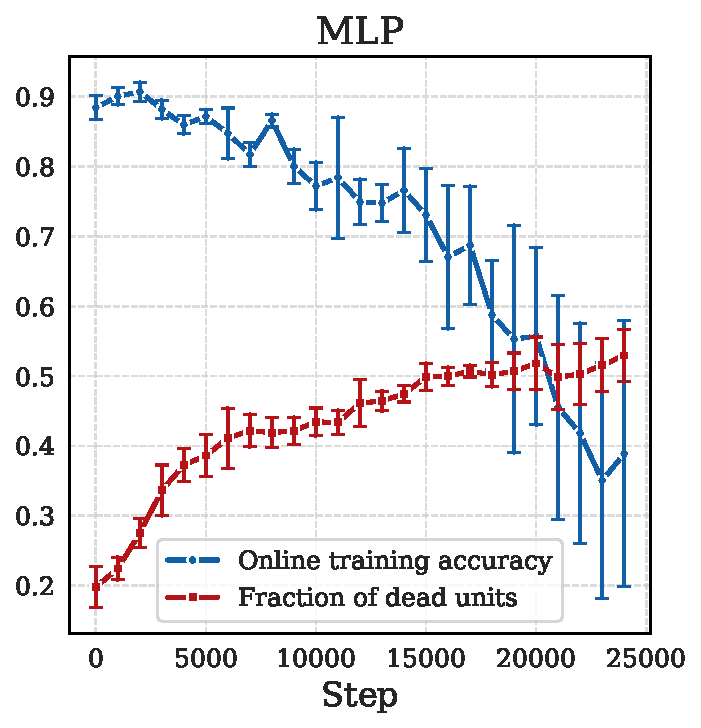
\includegraphics[width=0.23\linewidth]{mlp_act__dead_fraction_plot.pdf} % MLP dead fraction over time/tasks
    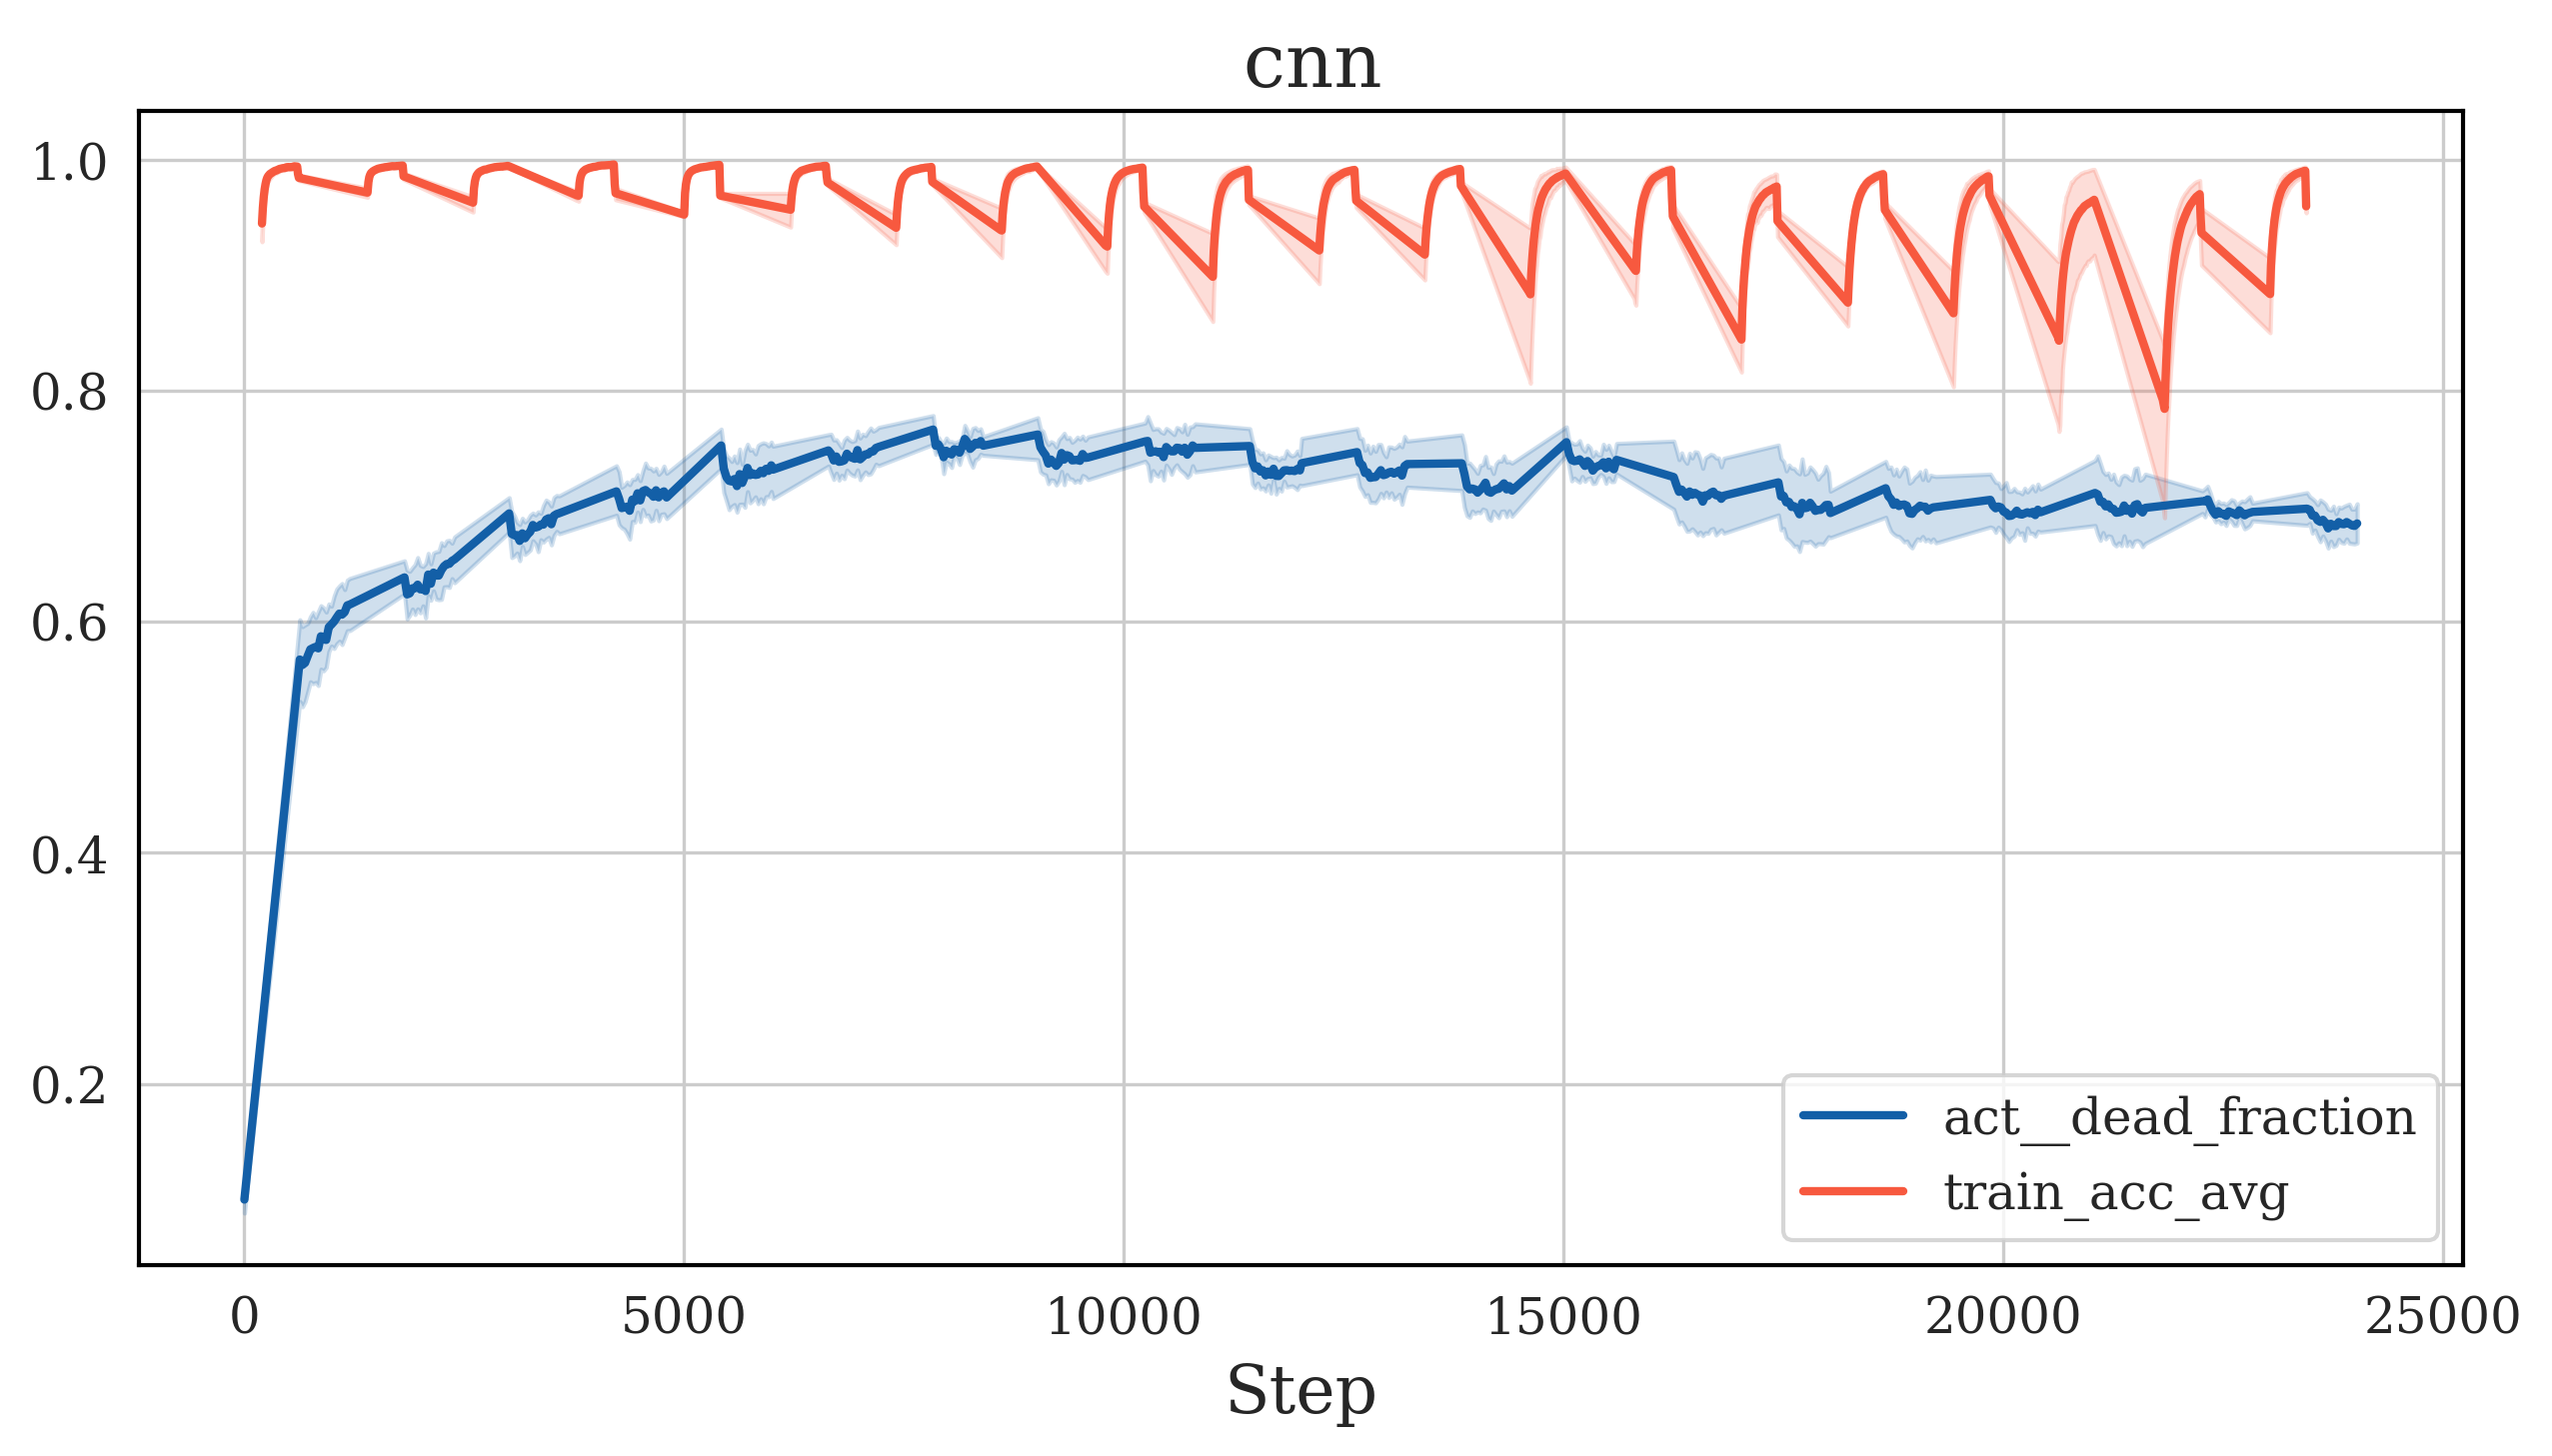
\includegraphics[width=0.38\linewidth]{dead_frac_cnn.png} % CNN dead fraction
    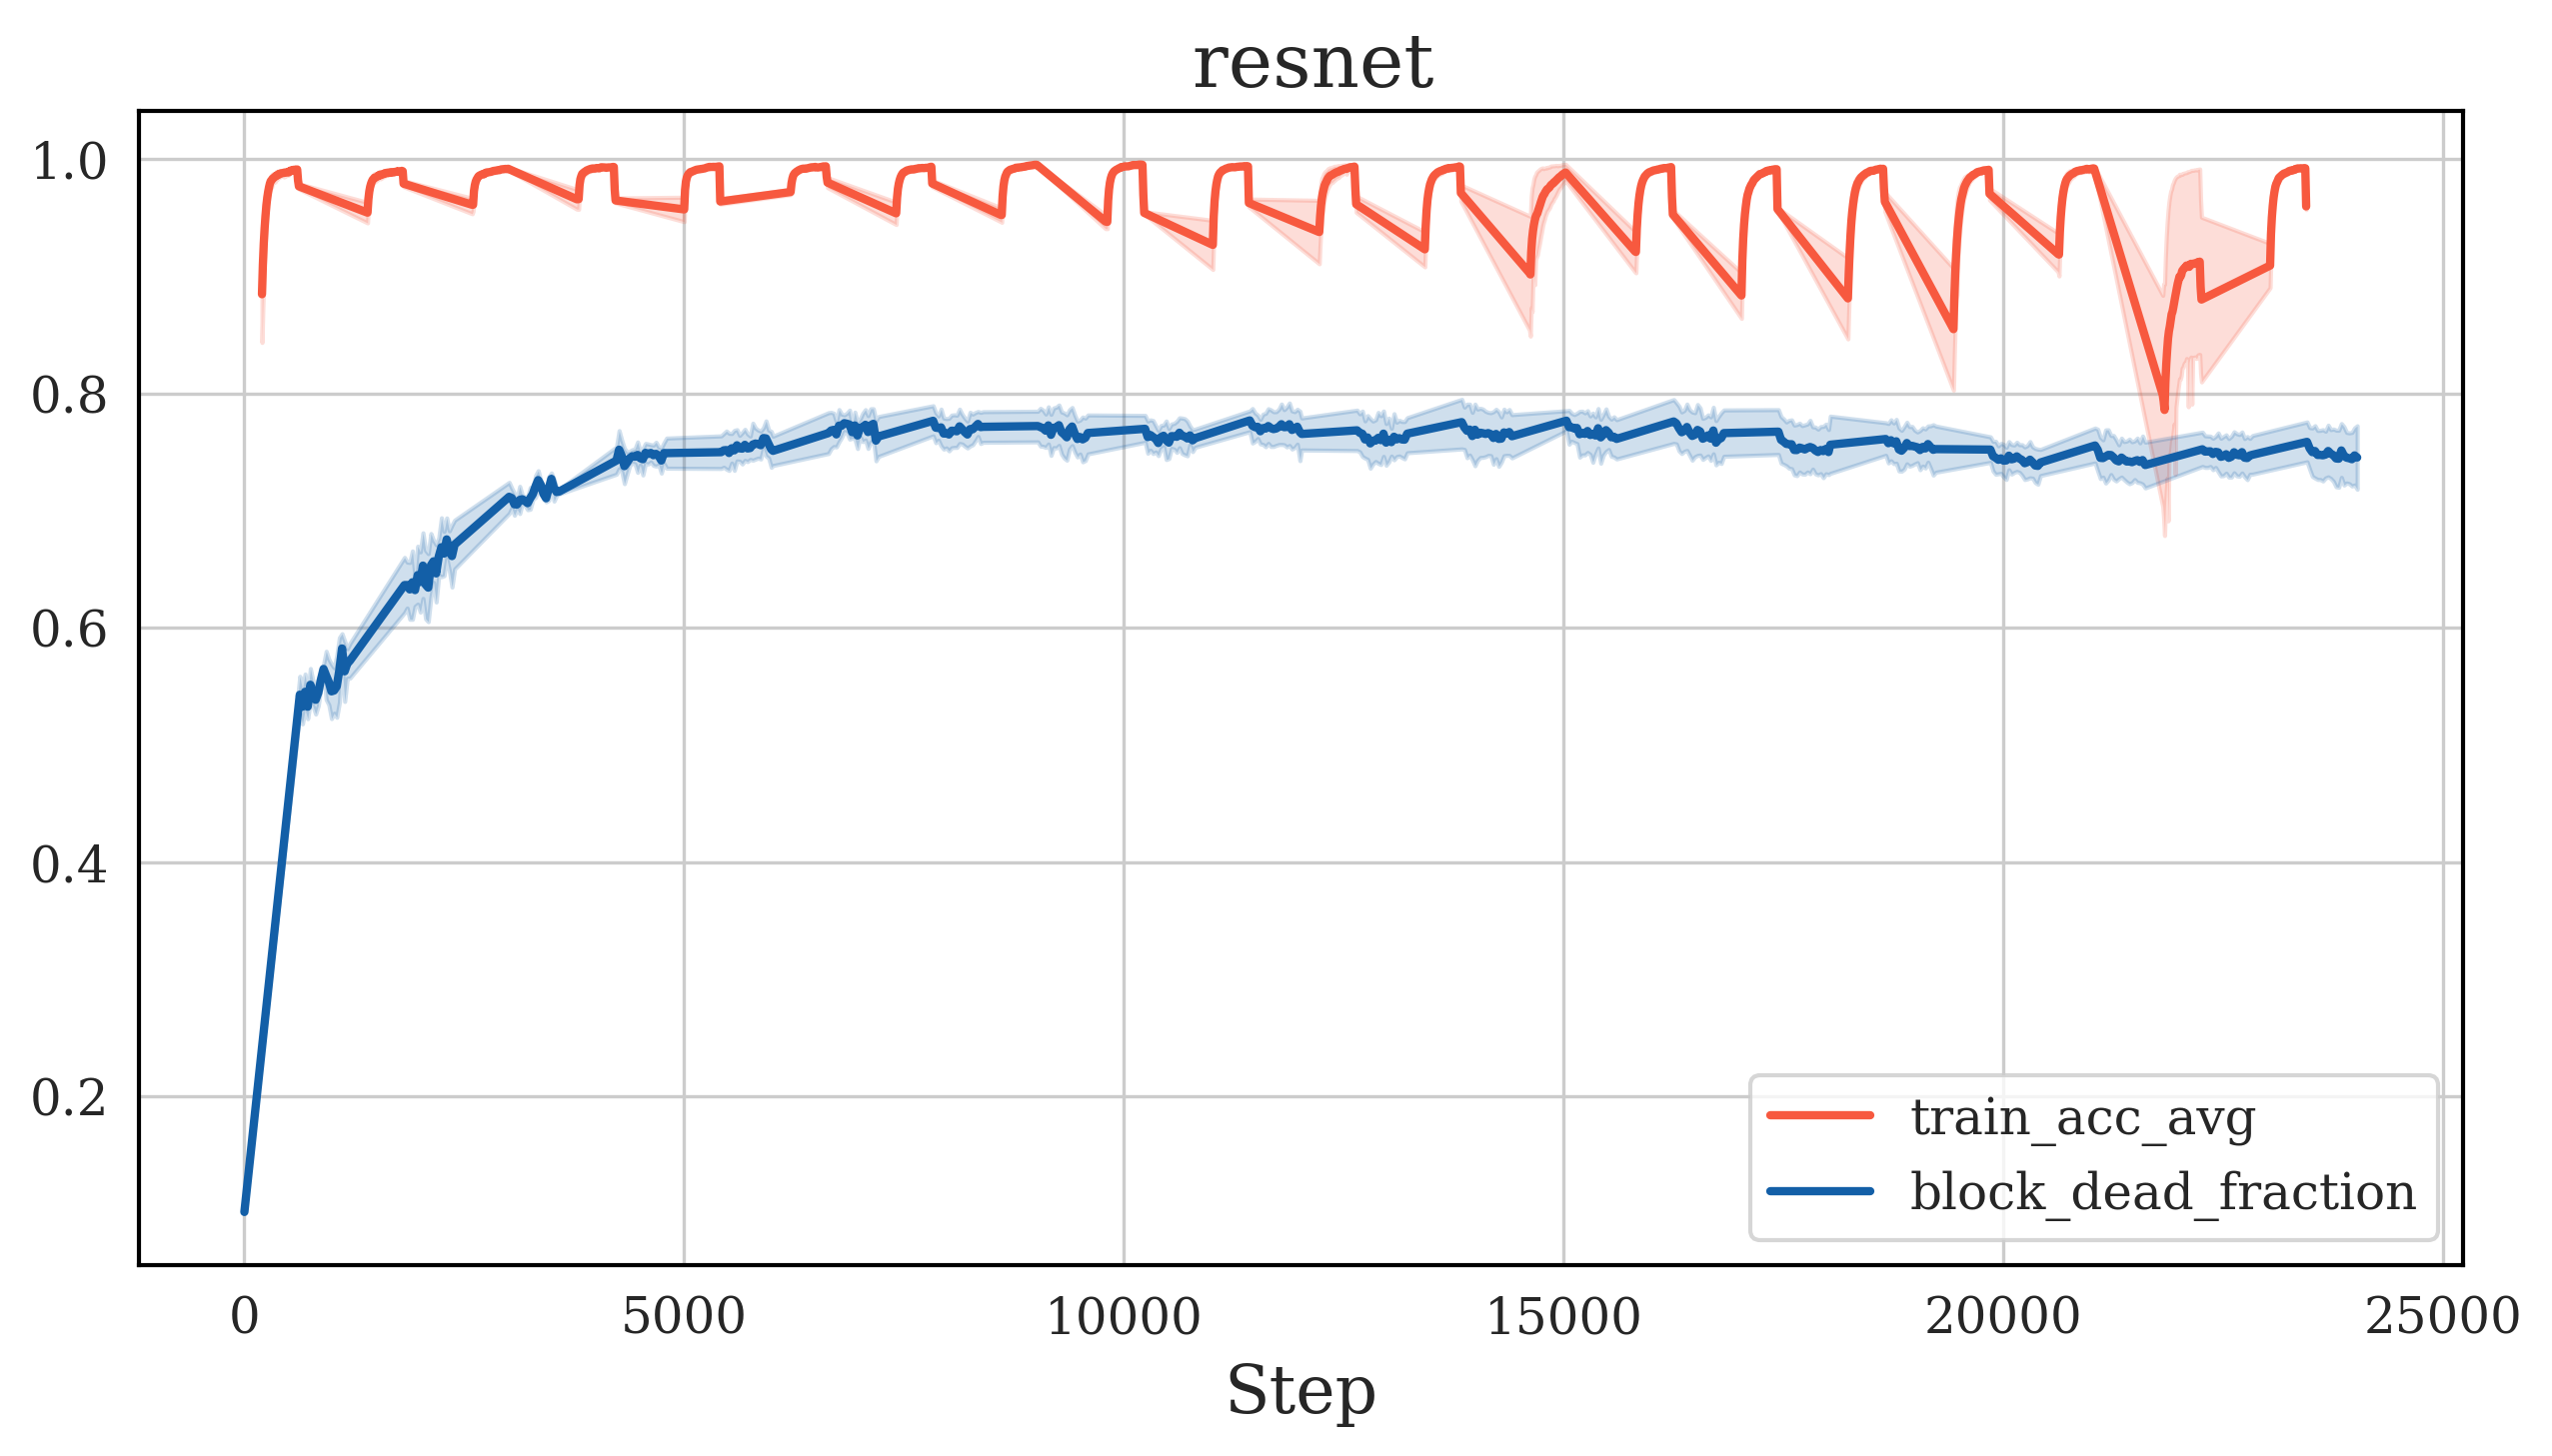
\includegraphics[width=0.38\linewidth]{dead_frac_resnet.png} % ResNet dead fraction
    % 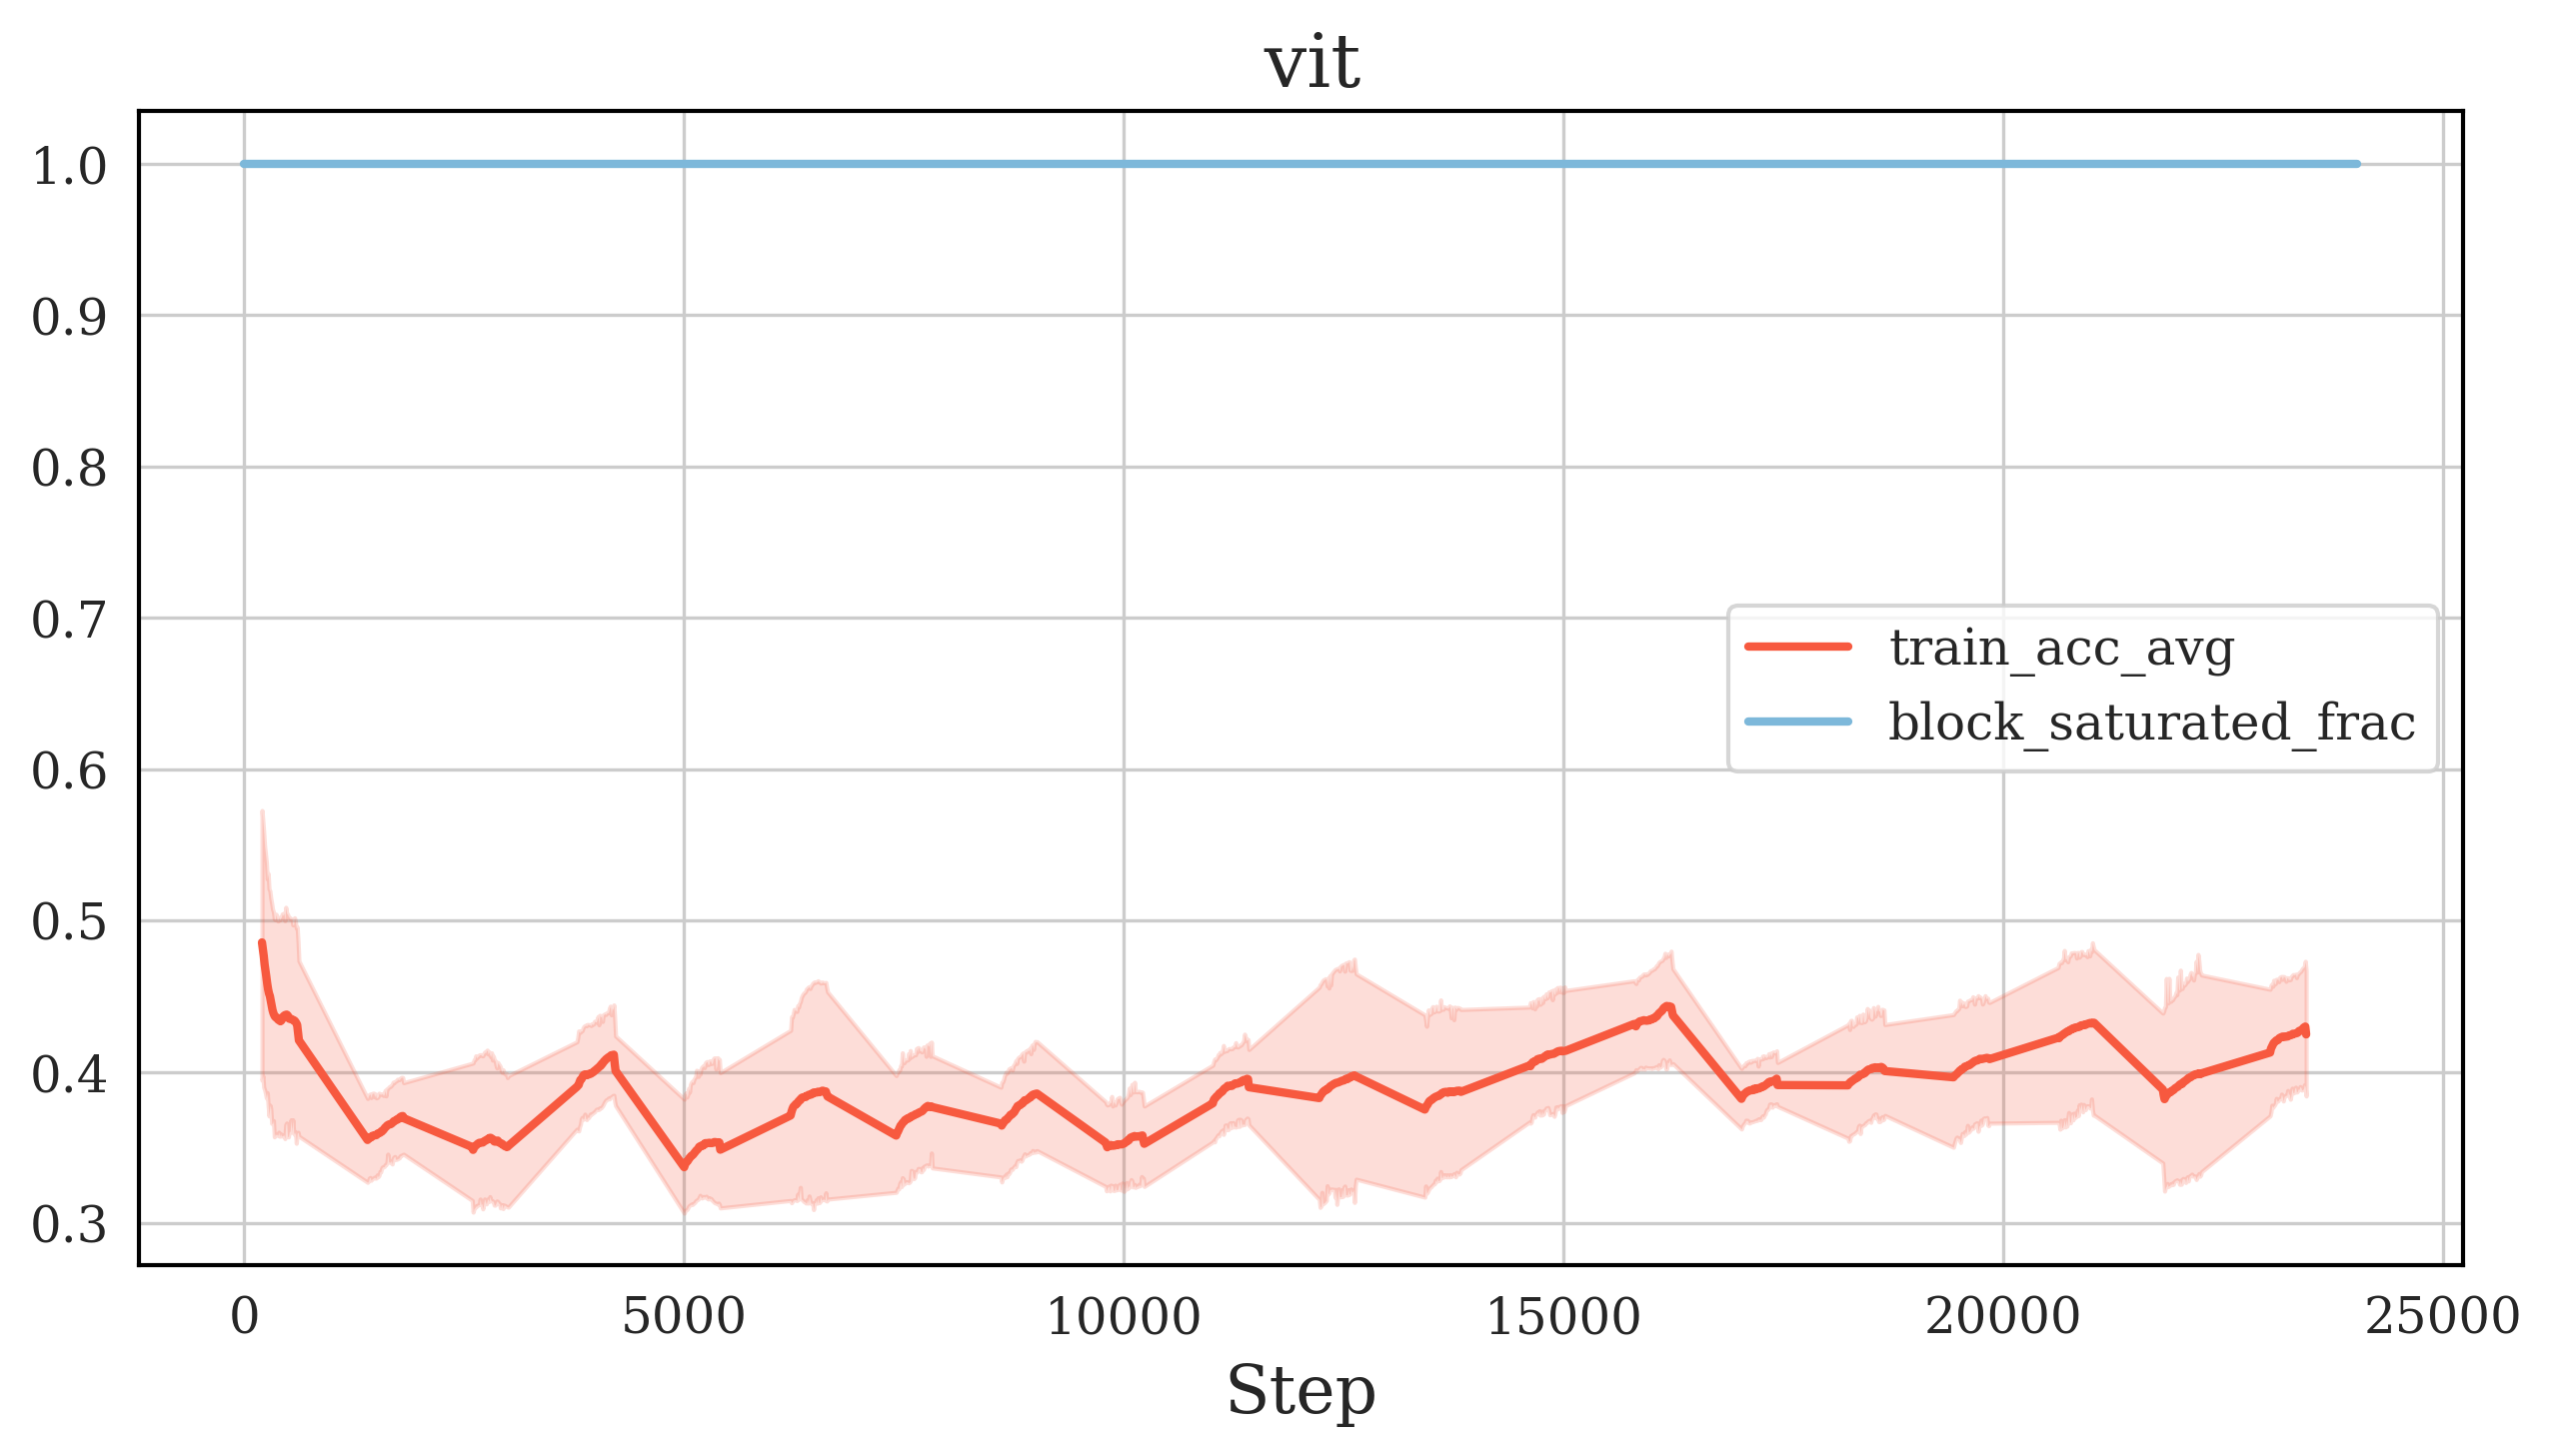
\includegraphics[width=0.4\linewidth]{sat_frac_vit.png} % ViT saturation - original figure, keeping separate if distinct from "dead"
    \caption{Emergence of unresponsive (dead/saturated) units during training across different architectures (MLP, CNN, ResNet). Plots typically show the fraction of such units over training time or tasks. The jaggedness in some curves (e.g., MLP plot if it shows accuracy alongside) can occur due to task switches in continual learning. (Placeholder figure, specific metrics and axes labels would be in final version).}
    \label{fig:DeadReLUs-LoP}
\end{figure}

\begin{figure}[h!]
    \centering
    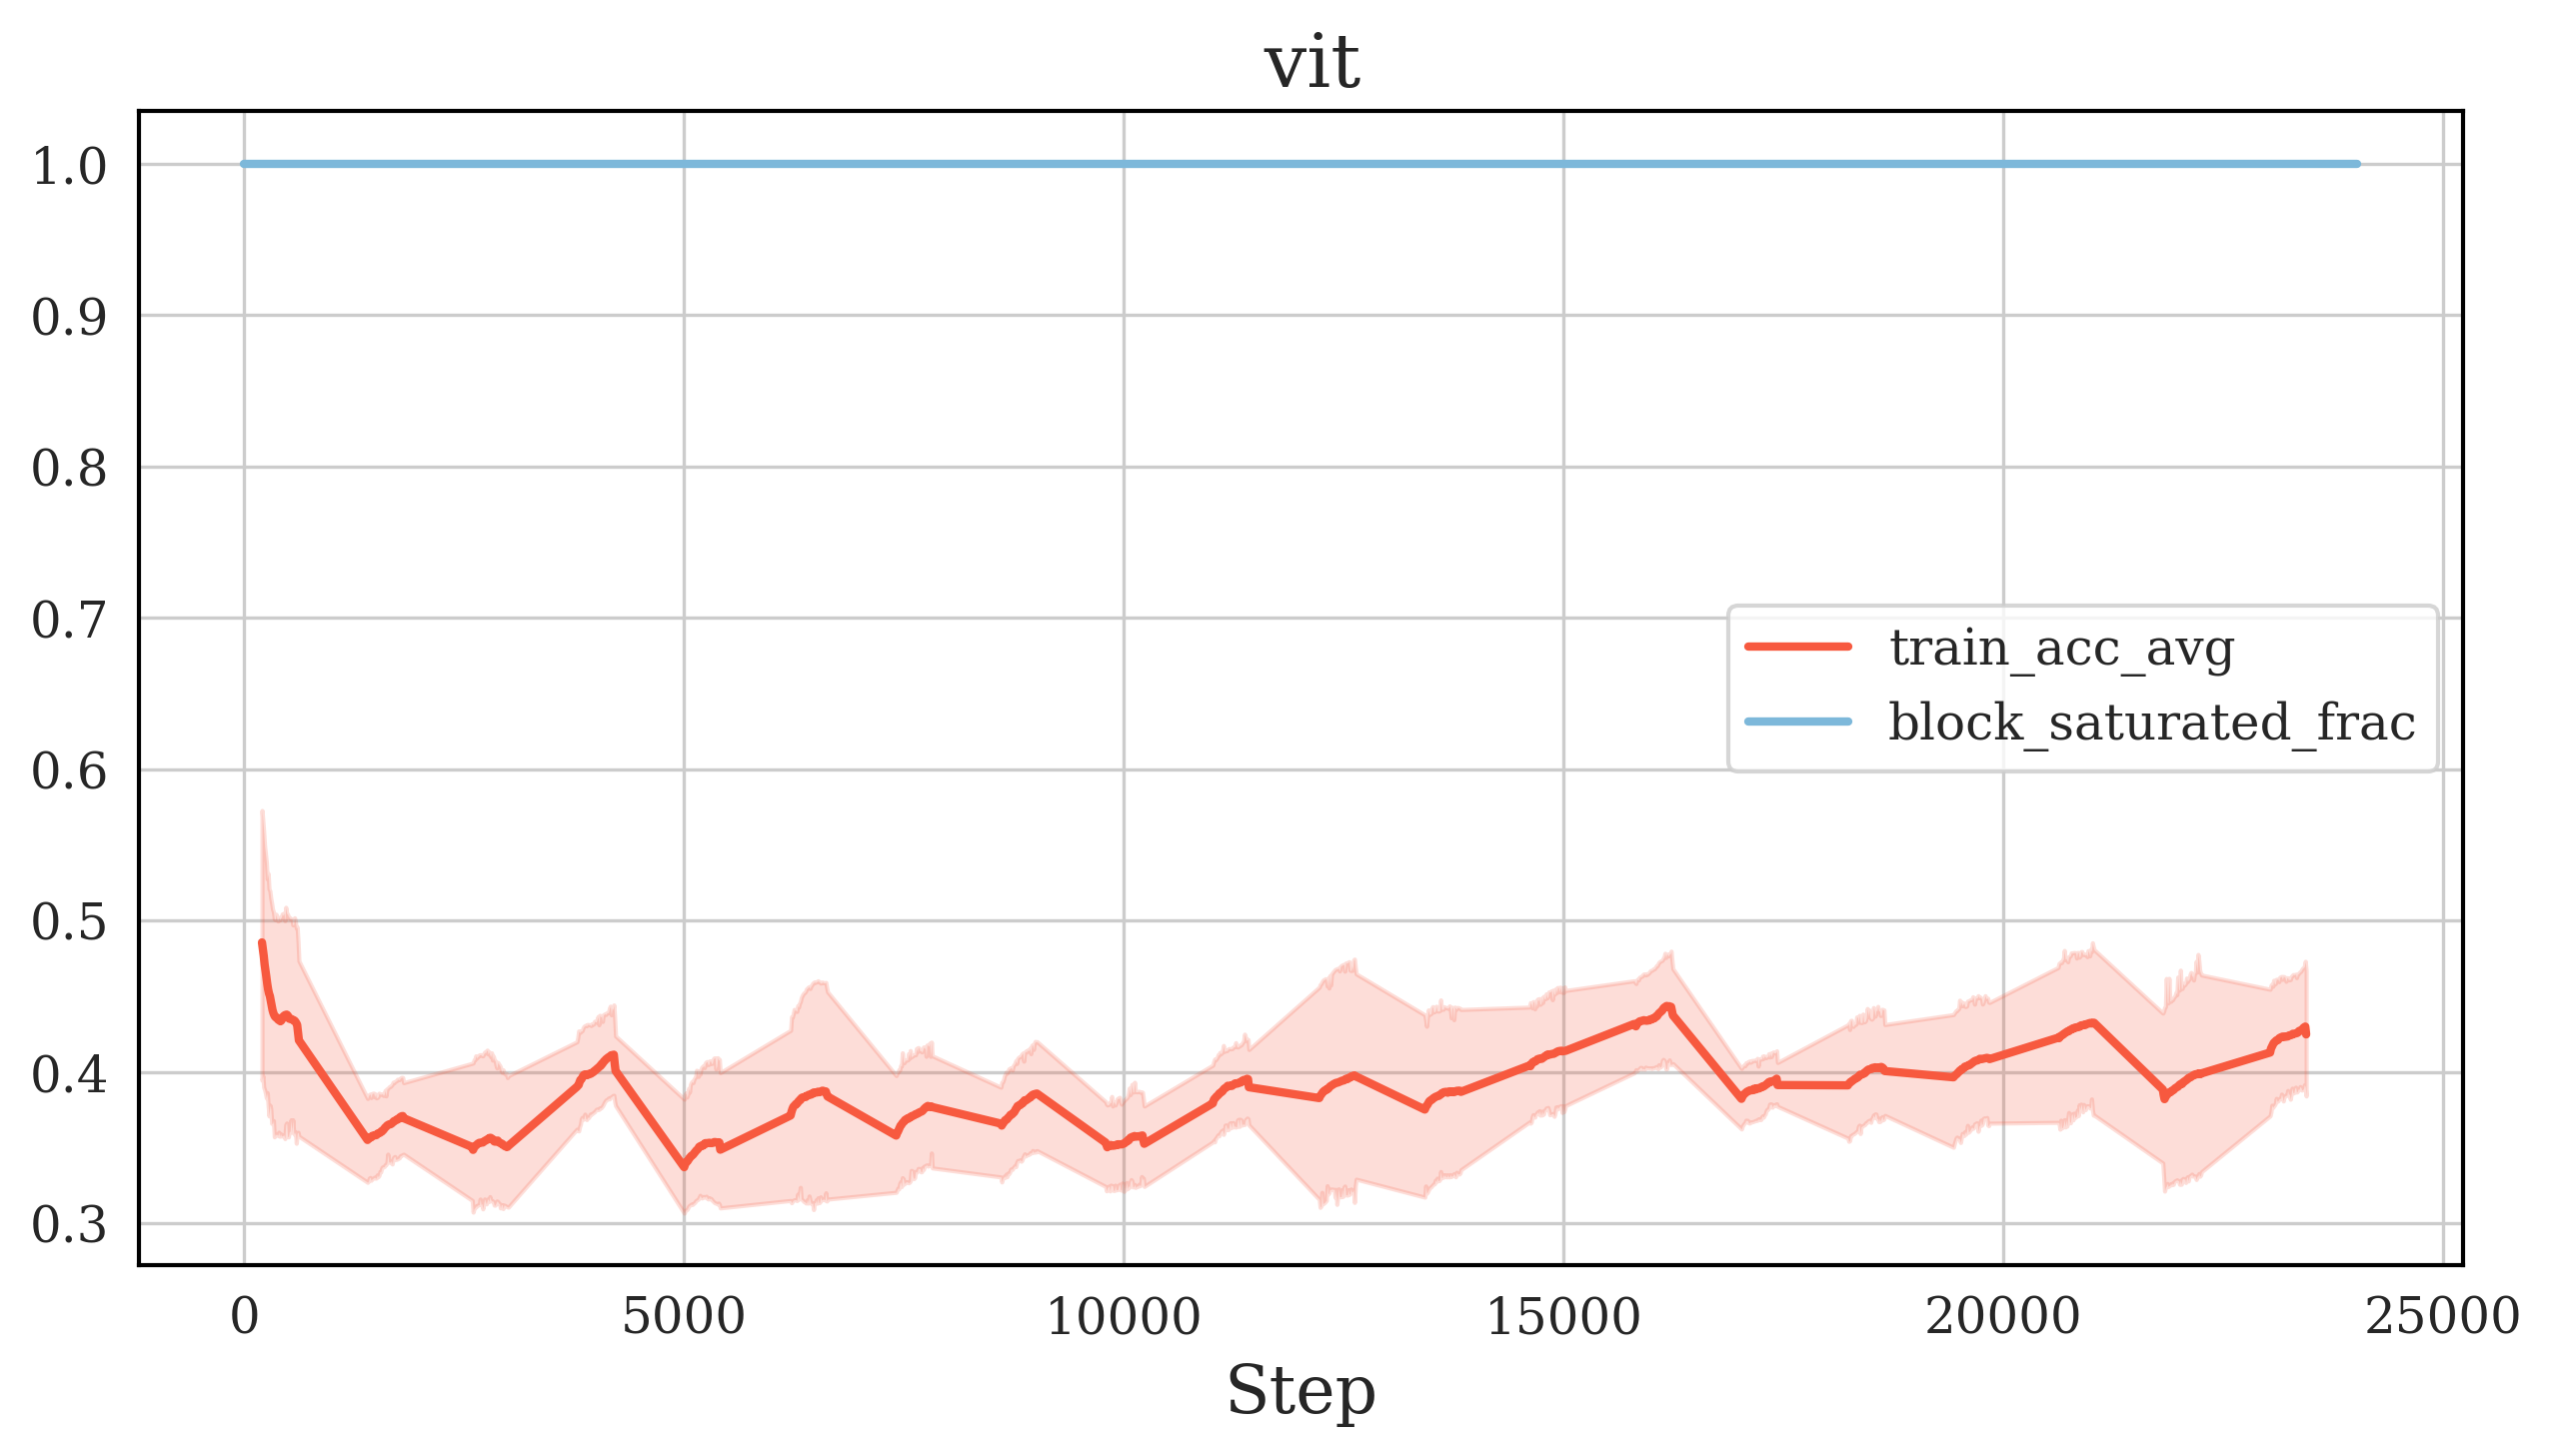
\includegraphics[width=0.4\linewidth]{sat_frac_vit.png} 
    \caption{Fraction of saturated units in a Vision Transformer (ViT) during training. (Placeholder figure, assumes layernorm is used as per original caption comment).}
    \label{fig:SatFracViT}
\end{figure}


\subsection{Structural LoP via Representational Redundancy: Cloned-Unit Manifolds}
\label{sec:cloned_units}
Plasticity can also diminish due to the emergence of redundant representations, where distinct sets of parameters learn to compute identical functions. This effectively reduces the network's functional size and its capacity to learn new, diverse features. We term manifolds arising from such redundancy ``cloned-unit manifolds.''

To formalize this, we consider a ``base'' network $G$ and a larger ``cloned'' network $\widetilde{G}$ where units or layers of $G$ are replicated in $\widetilde{G}$.
\begin{definition}[Block-wise Properties for Weight Matrices]
    Suppose $W$ is the $m \times n$ weight matrix of a layer in the base network $G$, and $\widetilde{W}$ is the corresponding $M \times N$ weight matrix in the cloned network $\widetilde{G}$. Let there be node coverings (partitions) $S_1, \dots, S_m$ of the $M$ input neurons and $T_1, \dots, T_n$ of the $N$ output neurons of this layer in $\widetilde{G}$, such that partition $S_i$ (or $T_j$) in $\widetilde{G}$ corresponds to input neuron $i$ (or output neuron $j$) in $G$. The submatrix $\widetilde{W}[S_i, T_j]$ in $\widetilde{G}$ corresponds to the weight $W_{ij}$ in $G$.
    \begin{itemize}
        \item $\widetilde{W}$ is \textbf{block-wise constant} if all elements within each block $\widetilde{W}[S_i, T_j]$ are equal to $W_{ij}/|S_i|$ (or some other consistent scaling ensuring equivalent sums).
        \item $\widetilde{W}$ has \textbf{row-equitable sums} if for any $u \in S_i$, $\sum_{v \in T_j} \widetilde{w}_{uv}$ is proportional to an effective outgoing weight from $i$ to $j$ in $G$. More specifically, for the proposition below, we often require that for each $u \in S_i$, $\sum_{v \in T_j} \widetilde{w}_{uv} = W_{ij}$ (if $G$'s weights $W_{ij}$ are from node $i$ to collection $j$).
        \item $\widetilde{W}$ has \textbf{column-equitable sums} if for any $v \in T_j$, $\sum_{u \in S_i} \widetilde{w}_{uv} = W_{ij}$ (if $G$'s weights $W_{ij}$ are from collection $i$ to node $j$).
    \end{itemize}
    For Proposition~\ref{prop:cloned}, the conditions are more specific, relating sums over cloned units to the corresponding single unit's weights in the base network.
\end{definition}

\begin{proposition}[Cloned-Unit Plasticity Loss]
\label{prop:cloned}
Let $G=(V,E,W)$ be a \emph{base} feed-forward network and $\widetilde{G}=(\widetilde{V},\widetilde{E},\widetilde{W})$ be a \emph{cloned} network. Suppose there is a surjective node mapping (a quotient map) $\pi: \widetilde{V} \to V$, defining partitions $S_i := \pi^{-1}(i) \subset \widetilde{V}$ for each $i \in V$. Assume activation functions $f_j$ are identical for all $\widetilde{u} \in S_j$.
If the initial weights $\widetilde{W}_0$ satisfy \emph{cloning conditions} such that:
\begin{enumerate}[label=(\roman*)]
    \item For any $\widetilde{u} \in S_i$, its outgoing connections to any partition $S_j$ are such that $\sum_{\widetilde{v} \in S_j, (\widetilde{u},\widetilde{v}) \in \widetilde{E}} \widetilde{w}_{\widetilde{u}\widetilde{v}} = w_{ij}$ (if $(i,j) \in E$, else 0).
    \item For any $\widetilde{v} \in S_j$, its incoming connections from any partition $S_i$ are such that $\sum_{\widetilde{u} \in S_i, (\widetilde{u},\widetilde{v}) \in \widetilde{E}} \widetilde{w}_{\widetilde{u}\widetilde{v}} = w_{ij}$ (if $(i,j) \in E$, else 0).
    % These conditions ensure that from the perspective of any single neuron in a partition, the summed influence from/to other partitions matches the base network.
\end{enumerate}
Then, under gradient descent (or common variants like SGD, Adam):
\begin{itemize}
    \item \textbf{Forward/Backward Symmetry:} For any input, all nodes $\widetilde{u}, \widetilde{v} \in S_i$ will have identical activations $h(\widetilde{u})=h(\widetilde{v})$ and identical error signals $\delta(\widetilde{u})=\delta(\widetilde{v})$ throughout training.
    \item \textbf{Gradient Symmetry:} The gradient $\nabla_{\widetilde{W}}\Loss$ will have a structure such that for any $i, j \in V$, all weights $\widetilde{w}_{\widetilde{u}\widetilde{v}}$ with $\widetilde{u} \in S_i, \widetilde{v} \in S_j$ will receive identical gradient components, meaning $\Delta \widetilde{w}_{\widetilde{u}\widetilde{v}}$ is the same for all these connections.
    \item \textbf{Manifold Confinement:} The parameter trajectory $\widetilde{W}(t)$ starting from $\widetilde{W}_0$ will remain confined to an affine subspace. This subspace is characterized by the initial cloning structure plus changes that preserve this structure. Effectively, $\widetilde{W}(t) - \widetilde{W}_0$ will maintain a block-wise constant structure (or more generally, a structure that preserves the sum-based cloning conditions). The dimension of this subspace is effectively that of the base network's parameters, $|E|$, which is typically much smaller than $|\widetilde{E}|$.
\end{itemize}
This represents a form of \emph{structural} LoP, as the larger network $\widetilde{G}$ is dynamically constrained to behave like the smaller network $G$, irrespective of the data distribution.
\end{proposition}

\paragraph{Intuition for Proposition~\ref{prop:cloned}:}
The core idea is that if a group of neurons in the cloned network starts identically (in terms of their weighted connections to other groups of identical neurons and their activation functions), they will process information identically and receive identical error signals. Consequently, their weights will be updated identically, preserving their cloned status. The network behaves as if these cloned neurons are just a single, more robust neuron from the base network. This is akin to an equitable partition in graph theory, where nodes within a block have the same number of neighbors in other blocks. The gradient flow respects this symmetry. The proof (details in Appendix~\ref{app:proofs}) formalizes this by induction.

This cloning phenomenon is not merely an artificial construct. Overparameterized networks can spontaneously develop such symmetries or near-symmetries during training, leading to a reduction in effective degrees of freedom. The modular version of cloning, mentioned in your notes and detailed in an appendix, allows constructing and verifying such cloned modules practically.

\begin{remark}
The affine subspace identified in Proposition~\ref{prop:cloned} acts as a stable LoP manifold for any optimizer relying solely on first-order gradient information (like SGD, Momentum, Adam) because the gradients themselves respect the cloning symmetry. This holds regardless of the data distribution. This is a powerful statement about the limitations imposed by such structures.
\end{remark}

\paragraph{Measuring Cloning:}
To quantify cloning, especially after a model is trained, the $R^2$ score can be adapted. For a layer with $N$ units partitioned into $B$ presumed cloned groups, let $A$ be the sum of squared deviations of unit activations (or weights) from their respective group means, and $B_{total}$ be the sum of squared deviations from the overall mean of all $N$ units. The cloning $R^2$ metric is $1 - A/B_{total}$. A value near 1 indicates strong cloning. This can be measured for both forward activations and backward-propagated gradients.

Figures~\ref{fig:dupfrac-LoP-emergence} (placeholder) are intended to show the emergence of duplicate units during training. Figure~\ref{fig:cloning_rank_loss} (placeholder) could show that the rank of layers remains similar after expansion if cloning conditions are met, and loss curves mirror this.

\begin{figure}[h!]
    \centering
    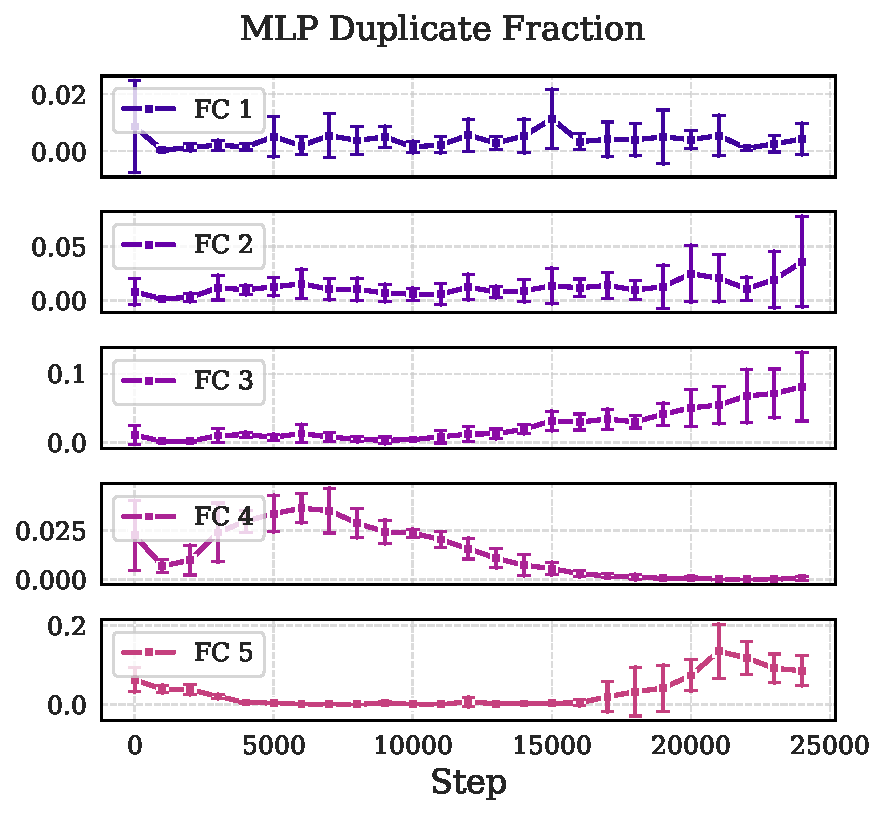
\includegraphics[width=0.24\linewidth]{mlp_act__dup_fraction_layerwise.pdf}
    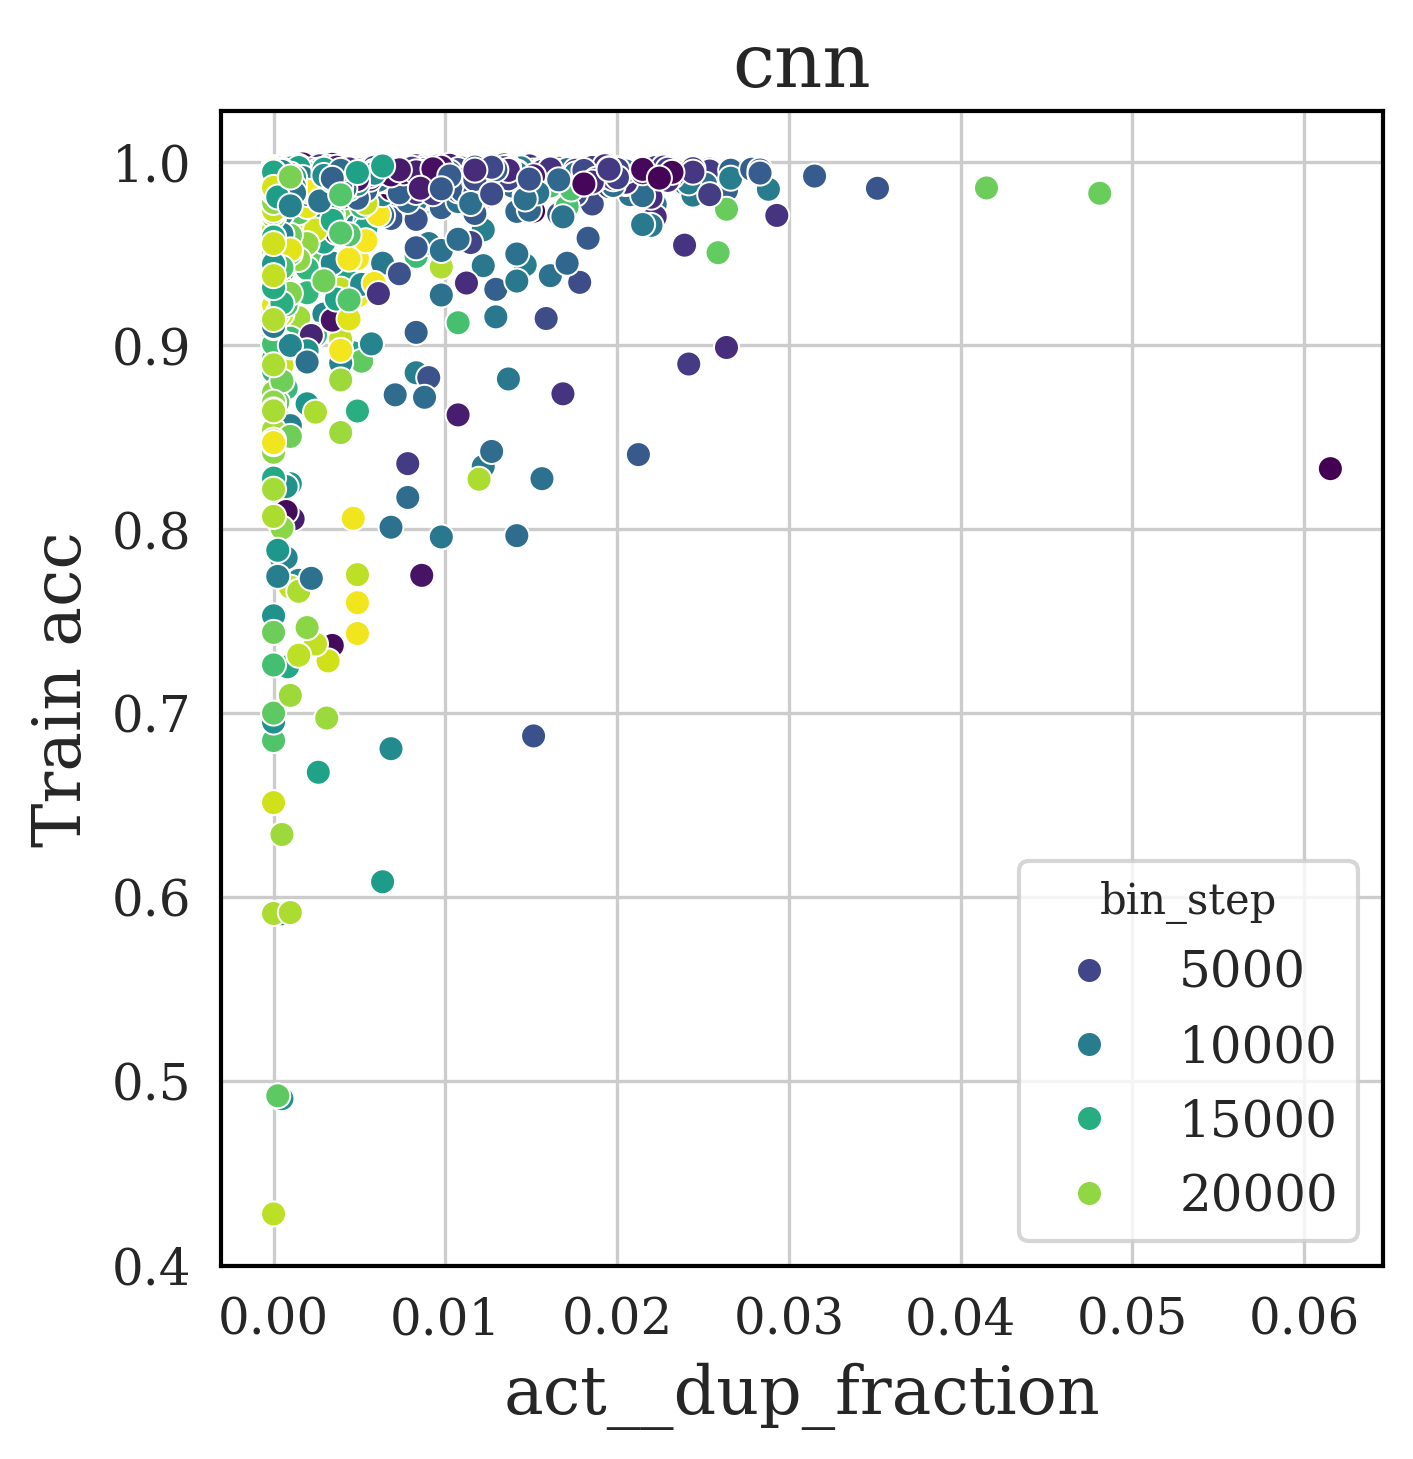
\includegraphics[width=0.24\linewidth]{cnn_dup_frac.png}
    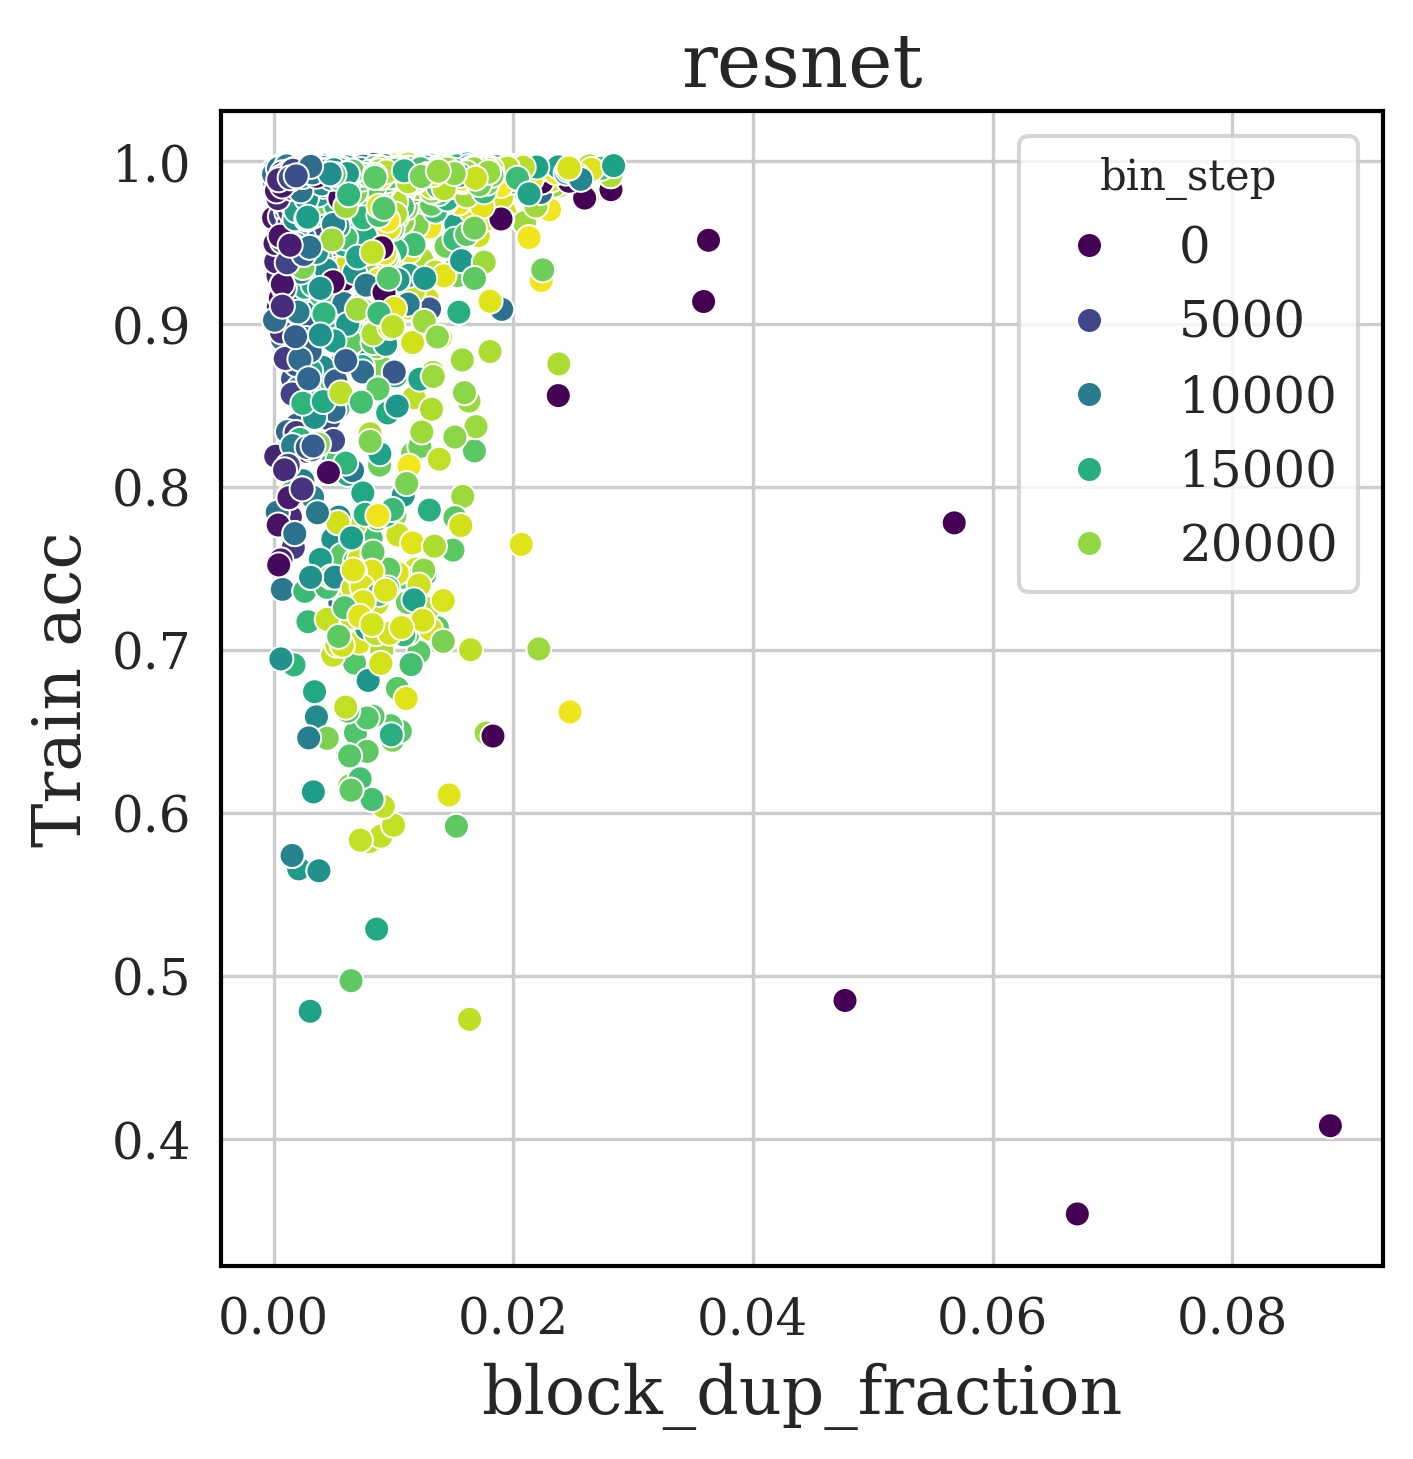
\includegraphics[width=0.24\linewidth]{resnet_dup_frac.png}
    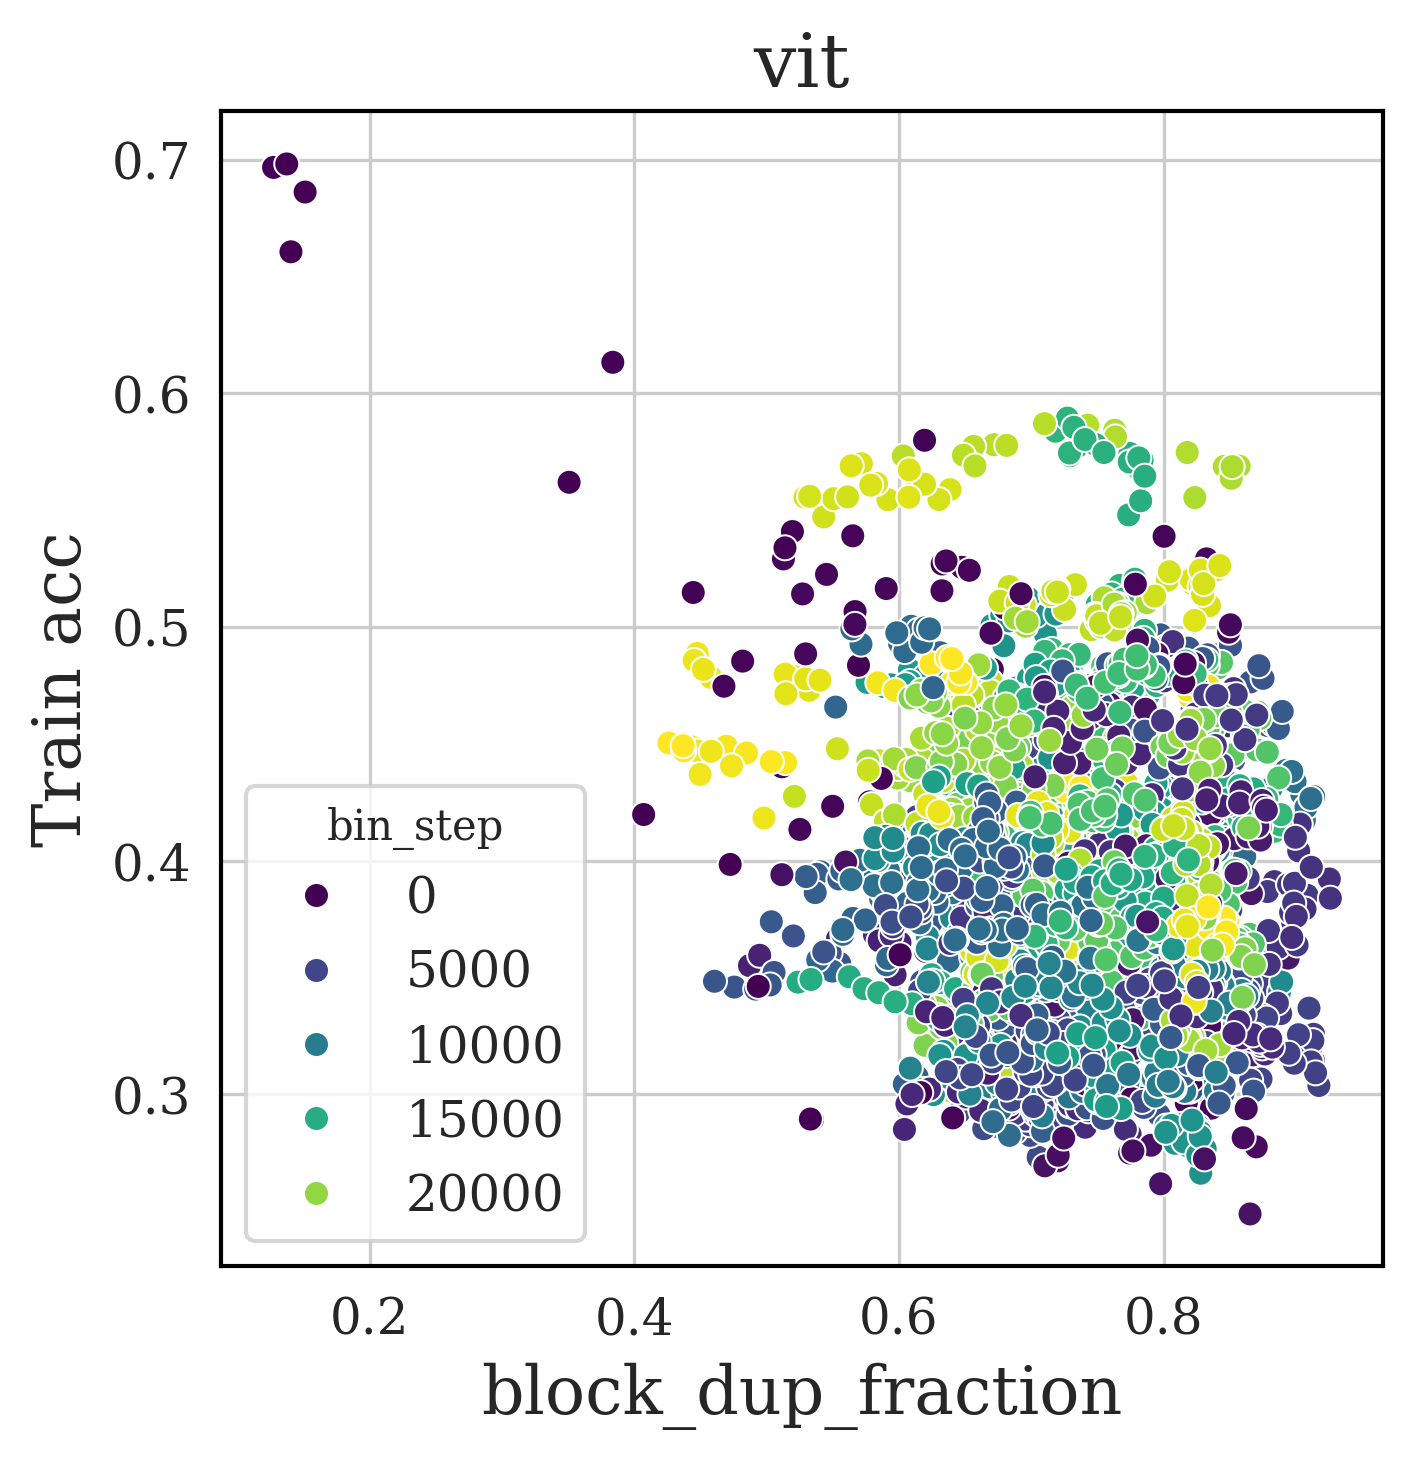
\includegraphics[width=0.24\linewidth]{vit_dup_frac.png}
    \caption{Emergence of duplicate units (or highly correlated units, indicating cloning) across layers in different architectures (MLP, CNN, ResNet, ViT) during training. Colors might represent different training stages. (Placeholder figure).}
    \label{fig:dupfrac-LoP-emergence}
\end{figure}

\begin{figure}[h!]
    \centering
    % Example of a figure that would support cloning claims, combining ideas from user notes
    % \includegraphics[width=0.4\linewidth]{cloned_model_rank_stability.pdf} 
    % \includegraphics[width=0.4\linewidth]{cloned_model_loss_curve.pdf}
    \caption{Illustrative results for cloning experiments. Left: Rank of representations in a cloned layer compared to a base model layer over training. Right: Training loss curves for a cloned model vs. its base model. Such plots would demonstrate that cloned models exhibit similar rank dynamics and learning trajectories as their smaller counterparts. (Placeholder figure based on user description).}
    \label{fig:cloning_rank_loss}
\end{figure}

The evolution of feature stable rank, as depicted in Figure~\ref{fig:stable_rank_evolution} (placeholder), often shows a decrease or stabilization at sub-optimal levels in networks prone to LoP, consistent with the emergence of low-rank phenomena like cloning.

\begin{figure}[h!]
    \centering
    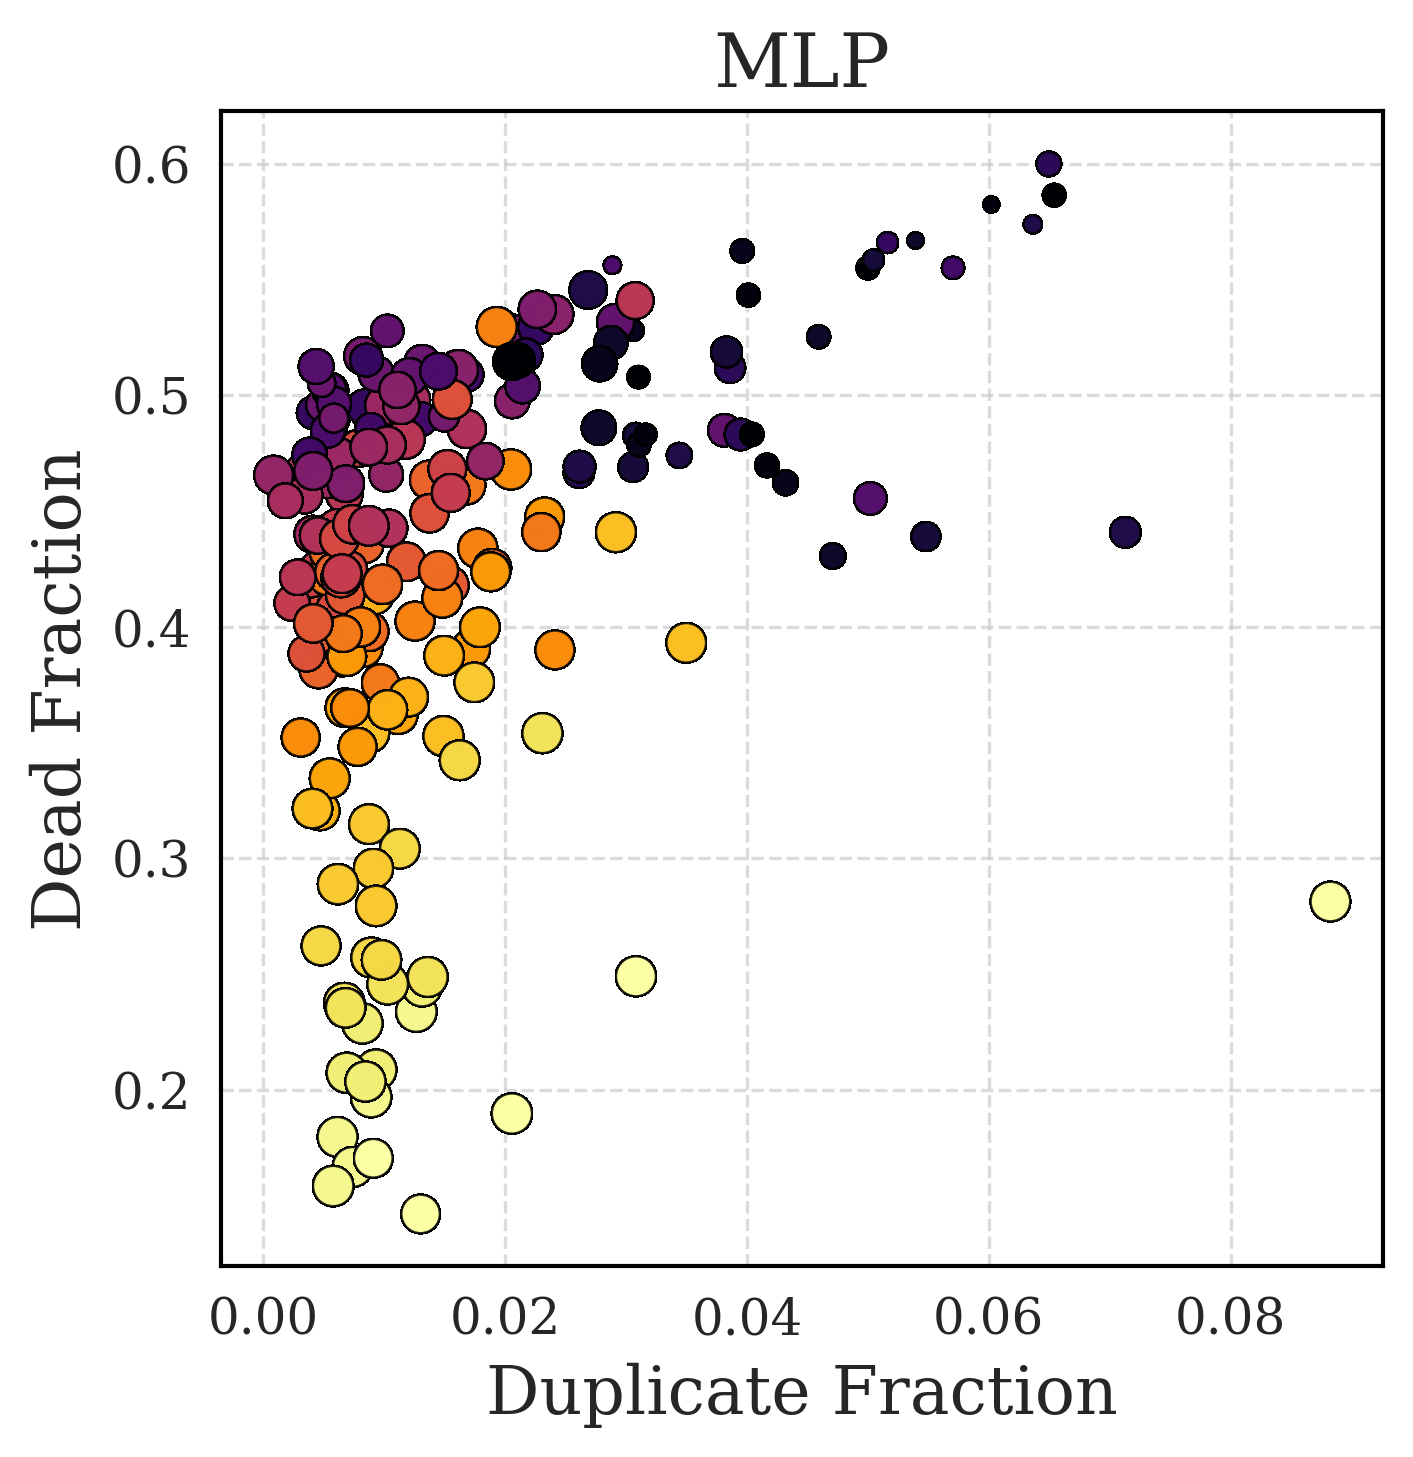
\includegraphics[width=0.24\linewidth]{mlp_dupdeadacc_plot.png} % This seems to combine dup/dead with accuracy
    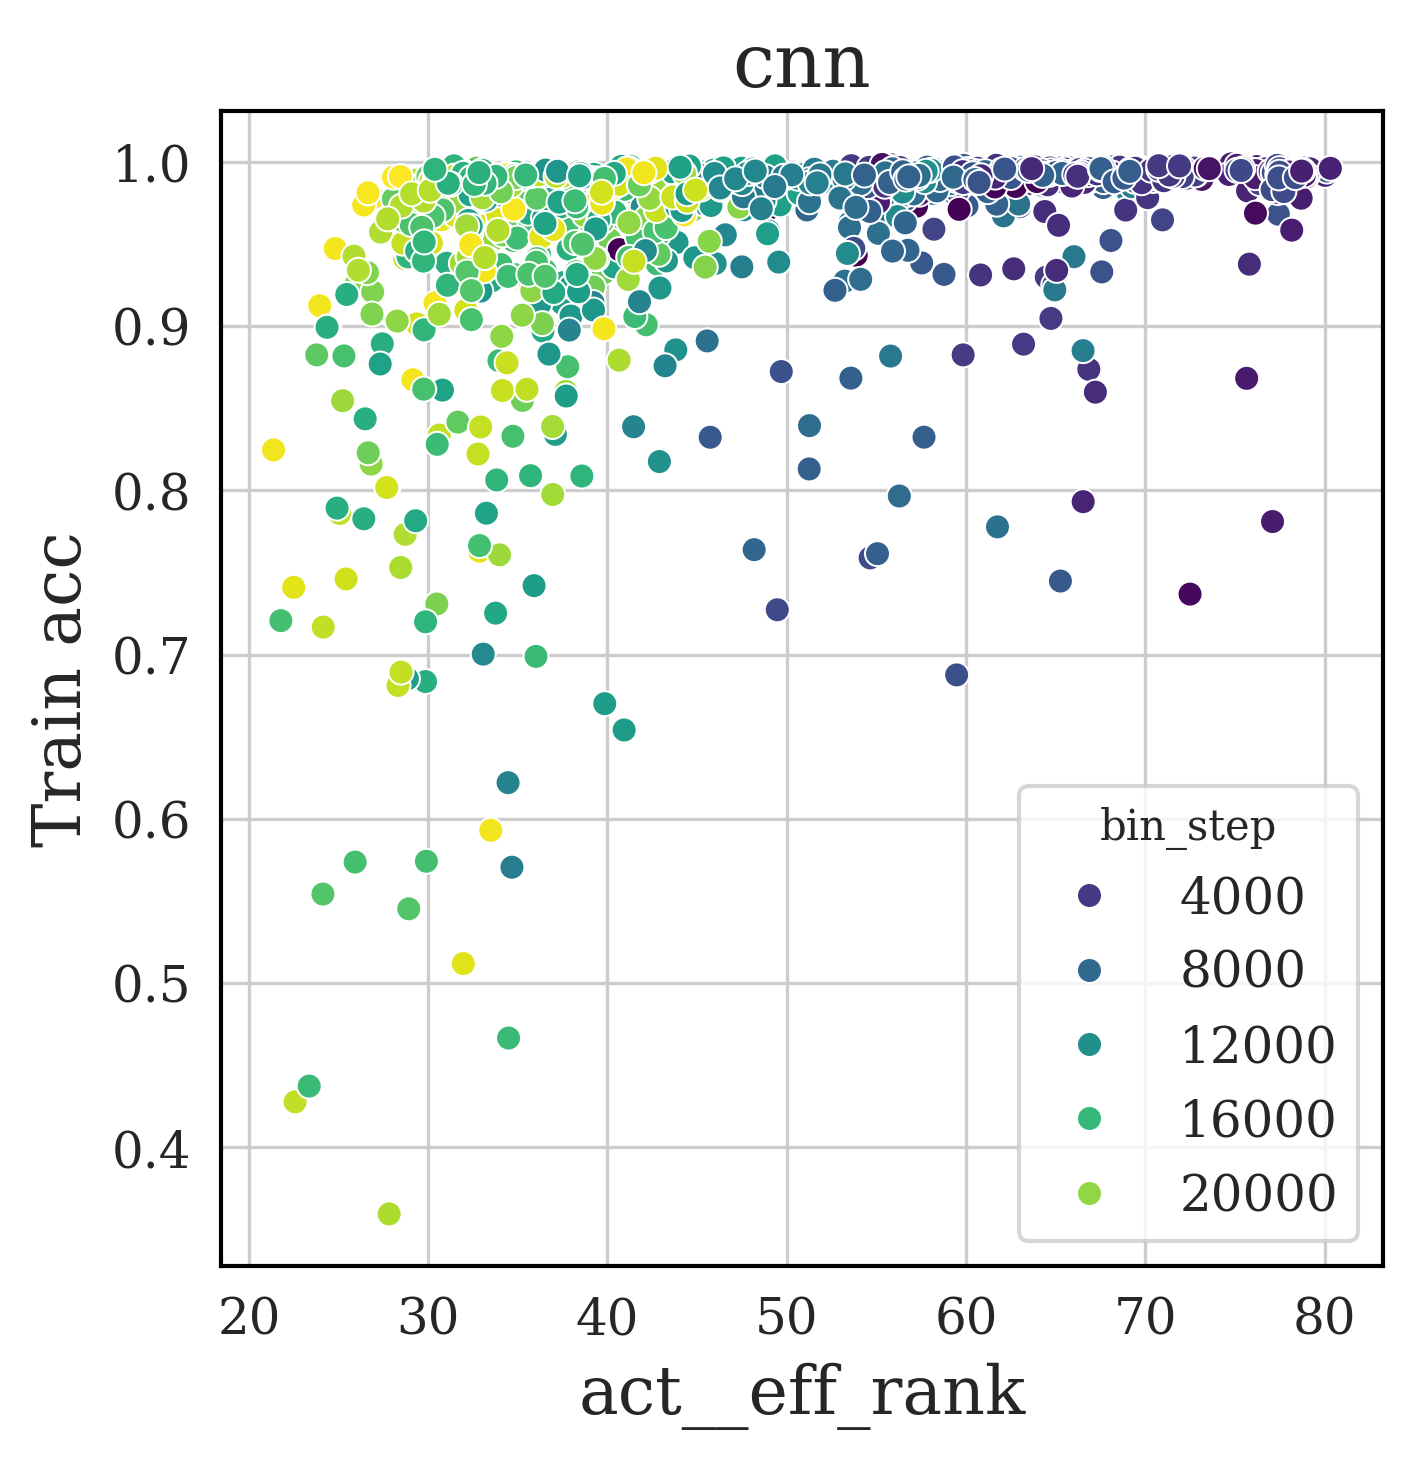
\includegraphics[width=0.24\linewidth]{cnn_stable_rank.png}
    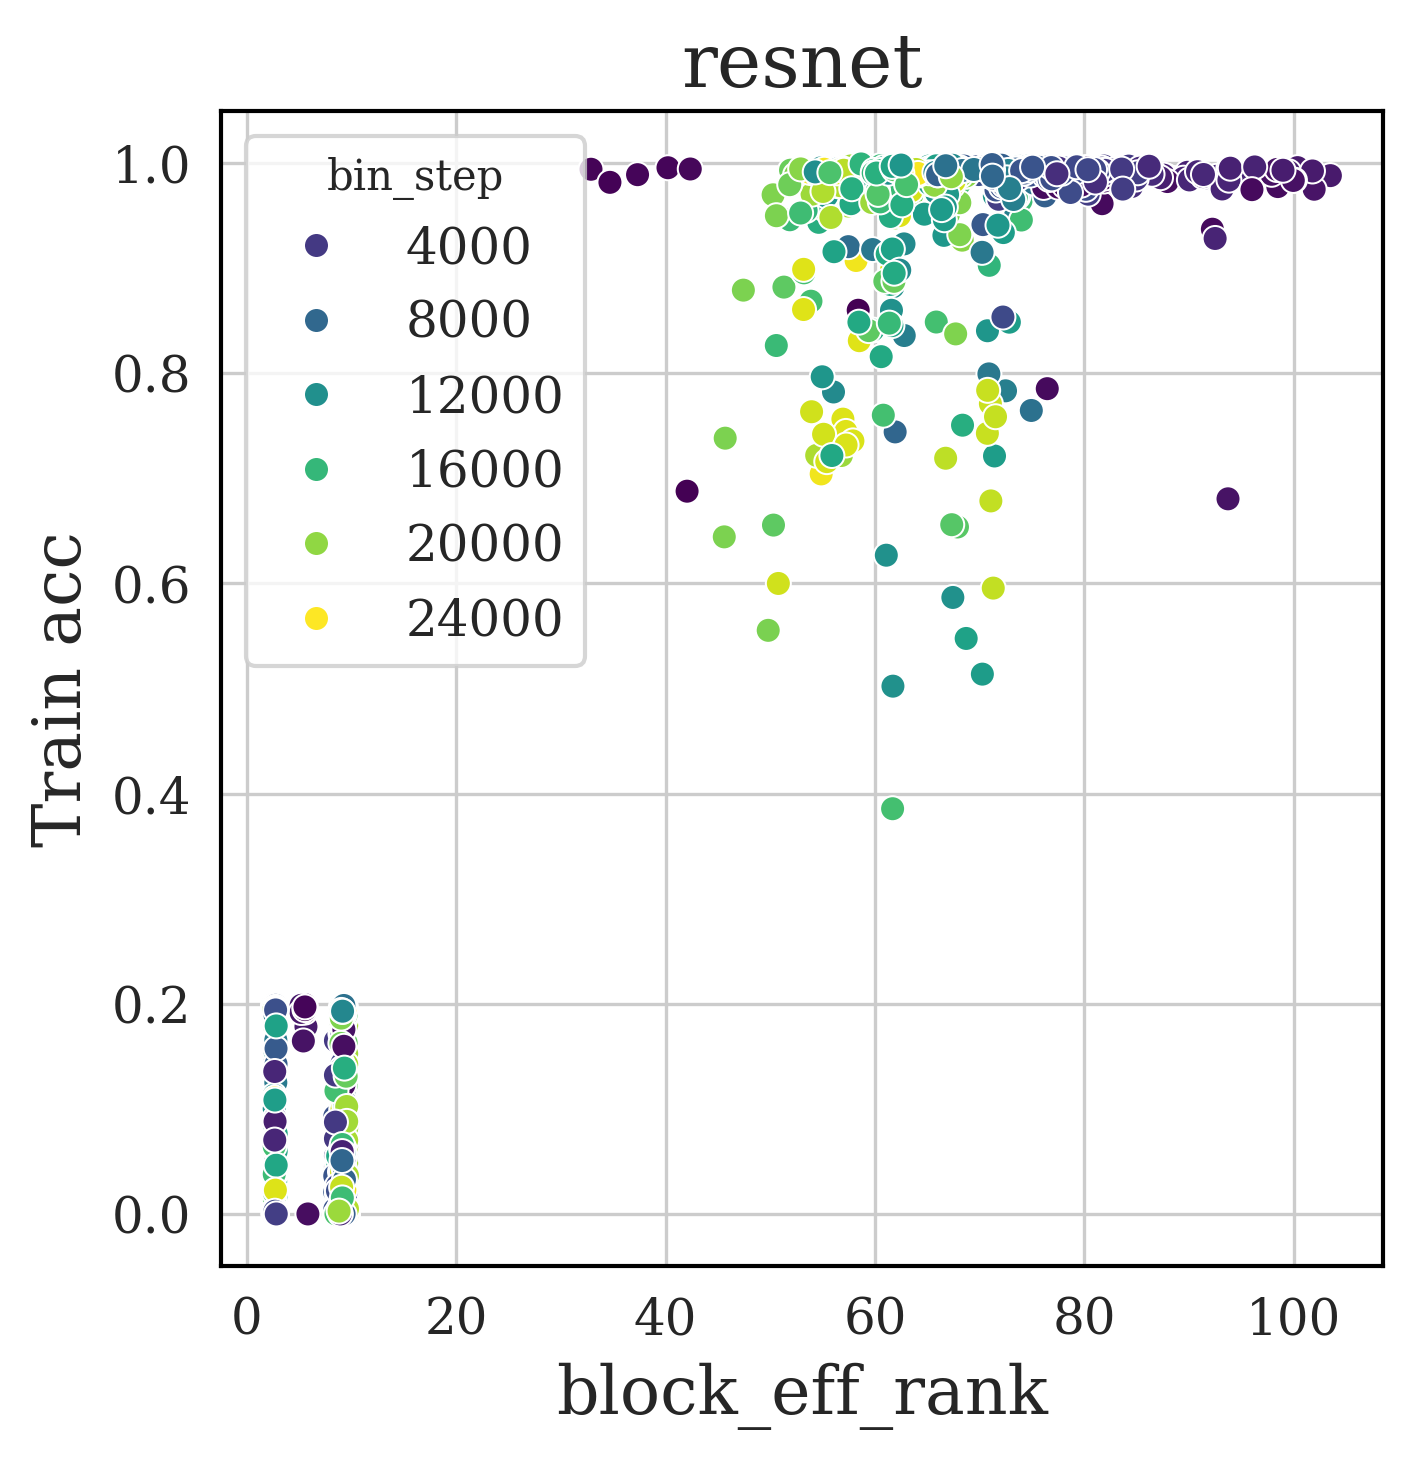
\includegraphics[width=0.24\linewidth]{resnet_stable_rank.png}
    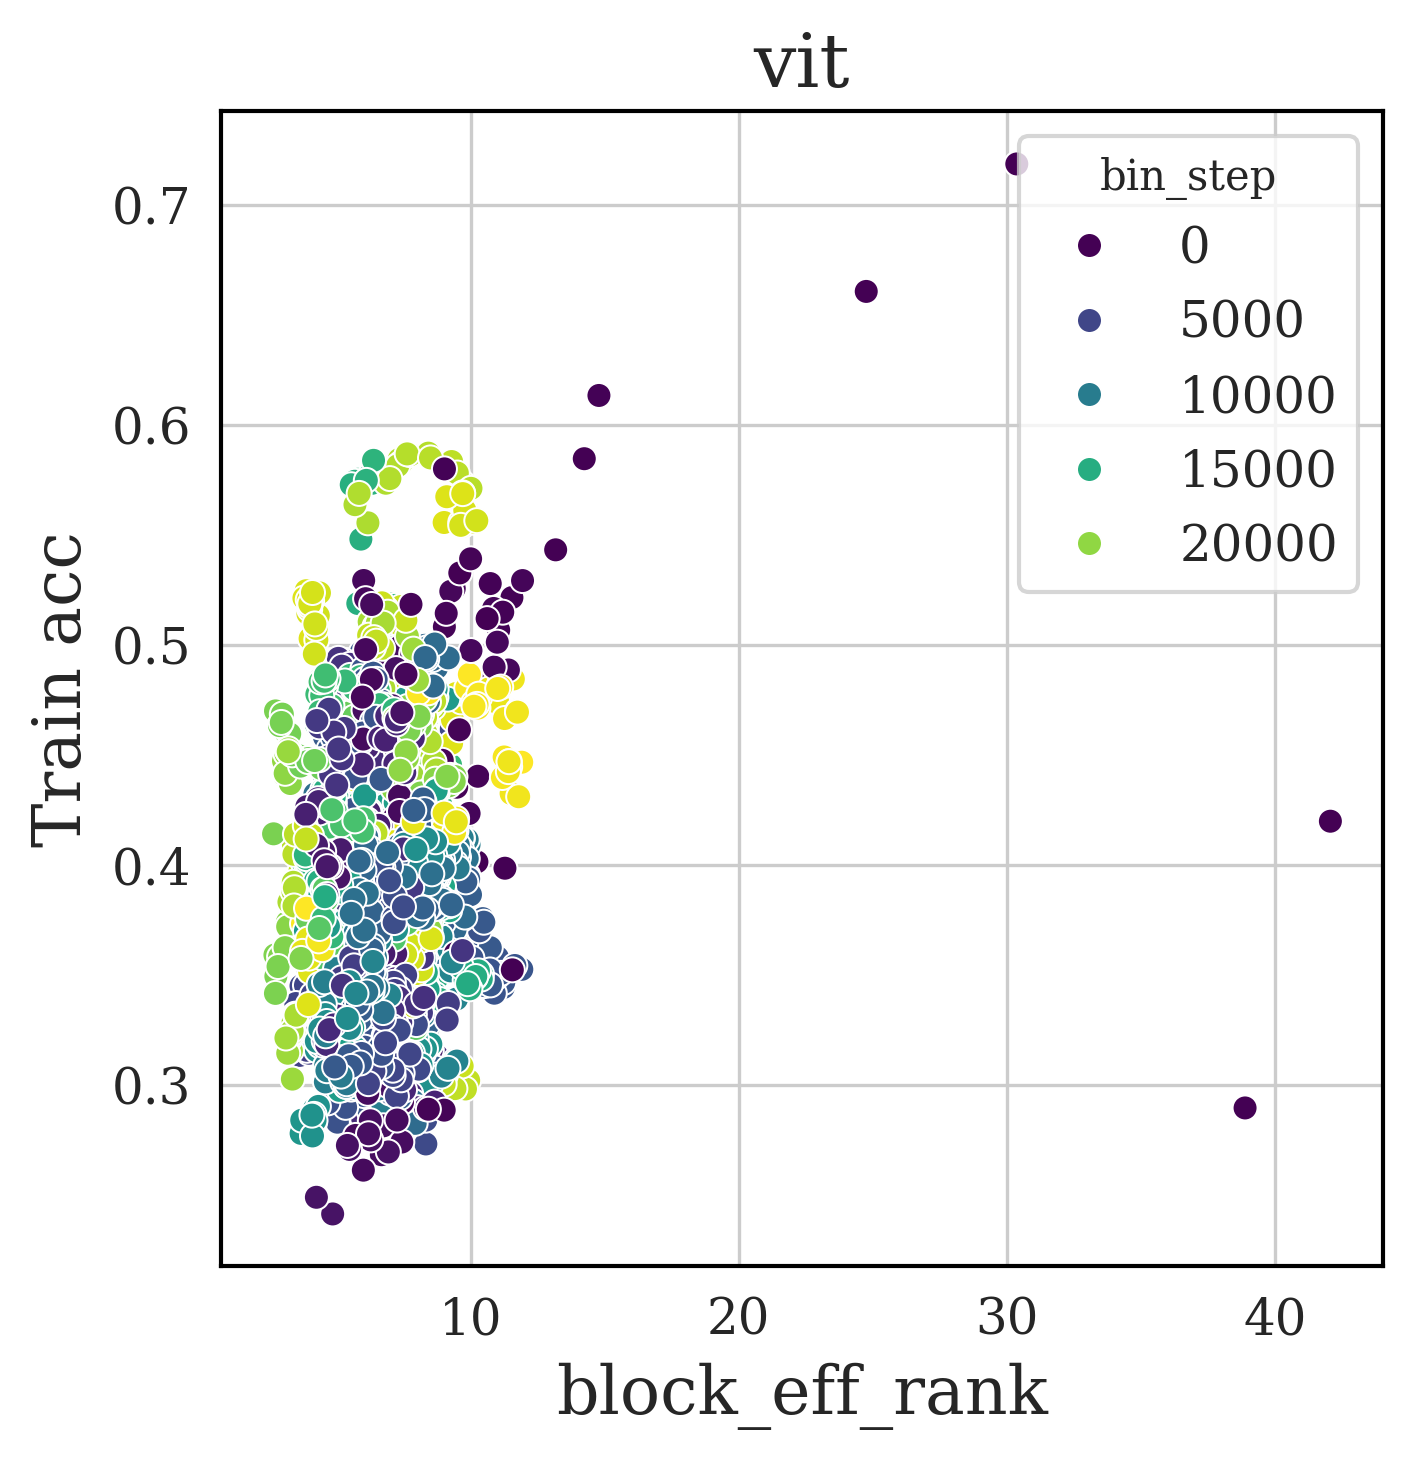
\includegraphics[width=0.24\linewidth]{vit_stable_rank.png}
    \caption{Evolution of stable rank of features during training for various architectures. Colors might represent training progression. A decline or plateau in stable rank can indicate emerging LoP. The MLP plot also relates duplicate/dead units to accuracy. (Placeholder figure).}
    \label{fig:stable_rank_evolution}
\end{figure}


\section{Mitigating Plasticity Loss and Escaping LoP Manifolds}
\label{sec:mitigate}

Understanding the mechanisms that lead to LoP manifolds—namely, the reduction of representational diversity through phenomena like unit saturation and cloning—naturally leads to exploring strategies to prevent confinement or facilitate escape from these restrictive states.

\subsection{Maintaining Representational Diversity}
A primary strategy to combat LoP is to actively maintain the richness and diversity of learned representations, particularly by preserving higher-rank feature spaces. Proposition~\ref{prop:rank_recovery_nonlinearity} established that non-linear activations are key to rank recovery. However, their effectiveness depends crucially on their operating regime, which is influenced by pre-activation statistics.

\paragraph{Role of Normalization and Activation Statistics:}
As discussed in Section~\ref{sec:feature_dynamics}, if pre-activations consistently fall into linear or saturated regions of an activation function, its ability to expand rank is diminished. For instance, Tanh behaves linearly for small inputs, and ReLU becomes affine for consistently positive inputs. Figures~\ref{fig:theory_tanh_az_rank}, \ref{fig:theory_relu_zb_rank} (Appendix~\ref{app:rank_validation_appendix_label}), and \ref{fig:theory_joint_norm_activation_rank} (Appendix~\ref{app:rank_validation_appendix_label}) synthetically demonstrate this dependence. These figures show that inappropriate scaling or shifting of pre-activations compromises the rank-recovery capacity of Tanh and ReLU.

Normalization techniques like Batch Normalization (BN) \citep{ioffe2015batch} and Layer Normalization (LN) aim to standardize pre-activation statistics (e.g., to zero mean and unit variance). This helps keep activations operating in their effective non-linear range, facilitating rank preservation and expansion. Figure~\ref{fig:empirical_rank_progression} empirically supports this by showing the progression of effective rank in MLPs with and without normalization. Models with BN or LN generally sustain higher effective rank across layers and epochs.
Figure~\ref{fig:norm-rank-nG} (placeholder) further explores the effect of normalization on effective rank and Gaussianity of activations.

\begin{figure}[ht!]
    \centering
    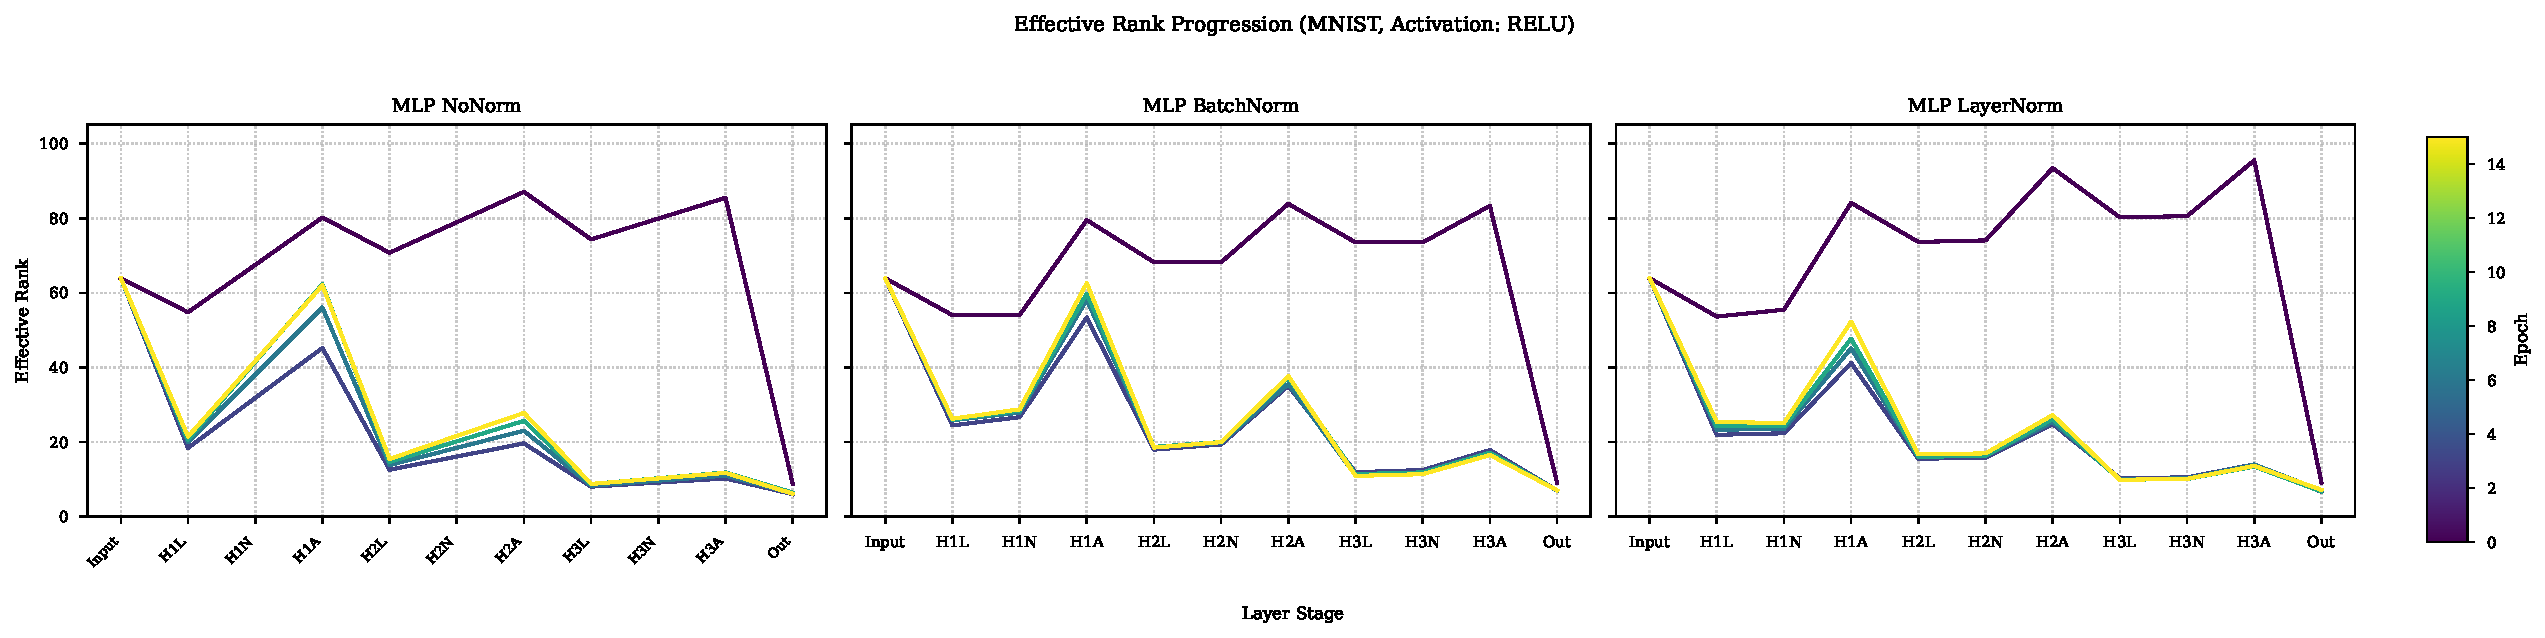
\includegraphics[width=\textwidth]{empirical_rank_progression_relu_mnist.pdf} 
    \caption{Empirical effective rank progression in an MLP trained on MNIST with ReLU activations. Subplots compare models with no normalization (left panel), Batch Normalization (center panel), and Layer Normalization (right panel). Lines within each subplot show the effective rank across network layers at different epochs (indicated by the color bar). Normalization generally helps maintain higher effective rank.}
    \label{fig:empirical_rank_progression}
\end{figure}

\begin{figure}[h!]
    \centering
    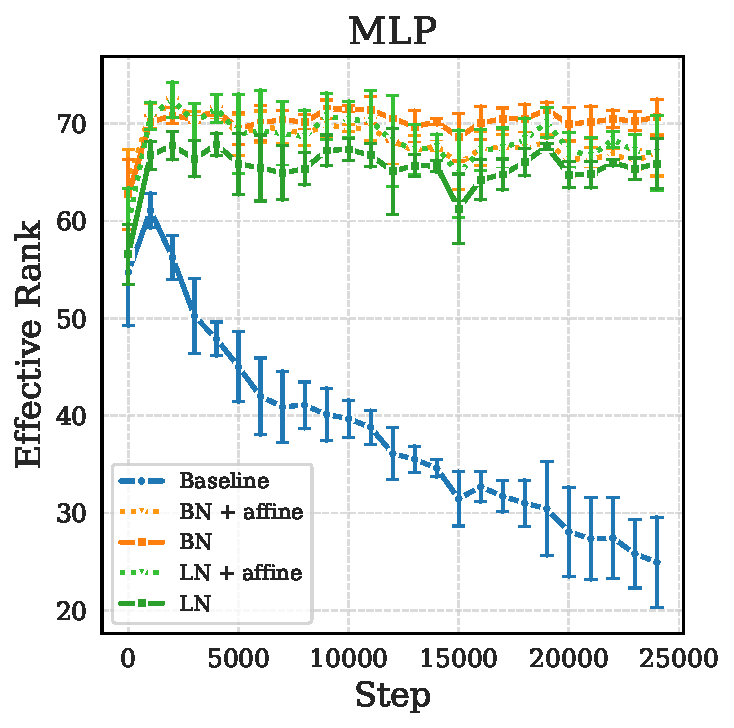
\includegraphics[width=0.24\linewidth]{mlp_act__eff_rank_normalizations_plot.pdf}
    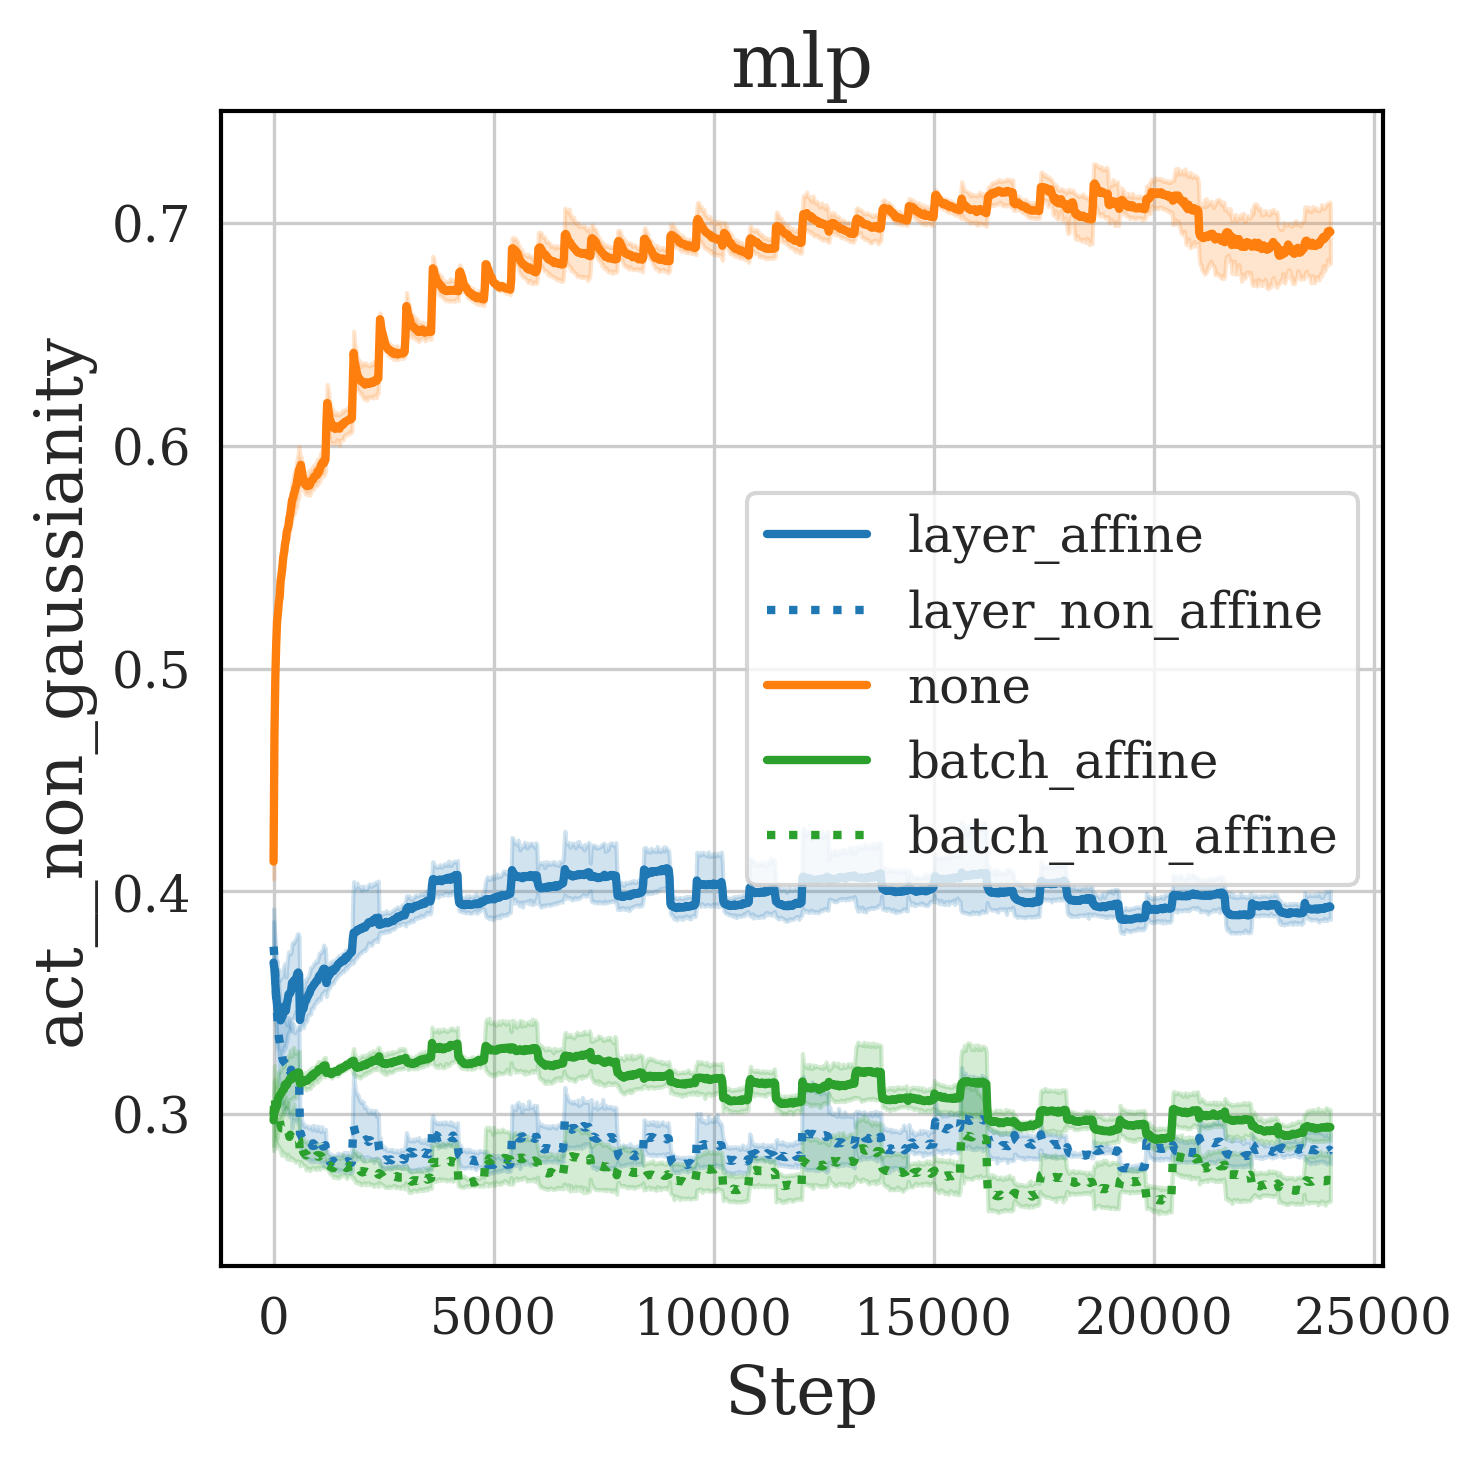
\includegraphics[width=0.24\linewidth]{mlp_nonGaussnorm.png} % Gaussianity for MLP
    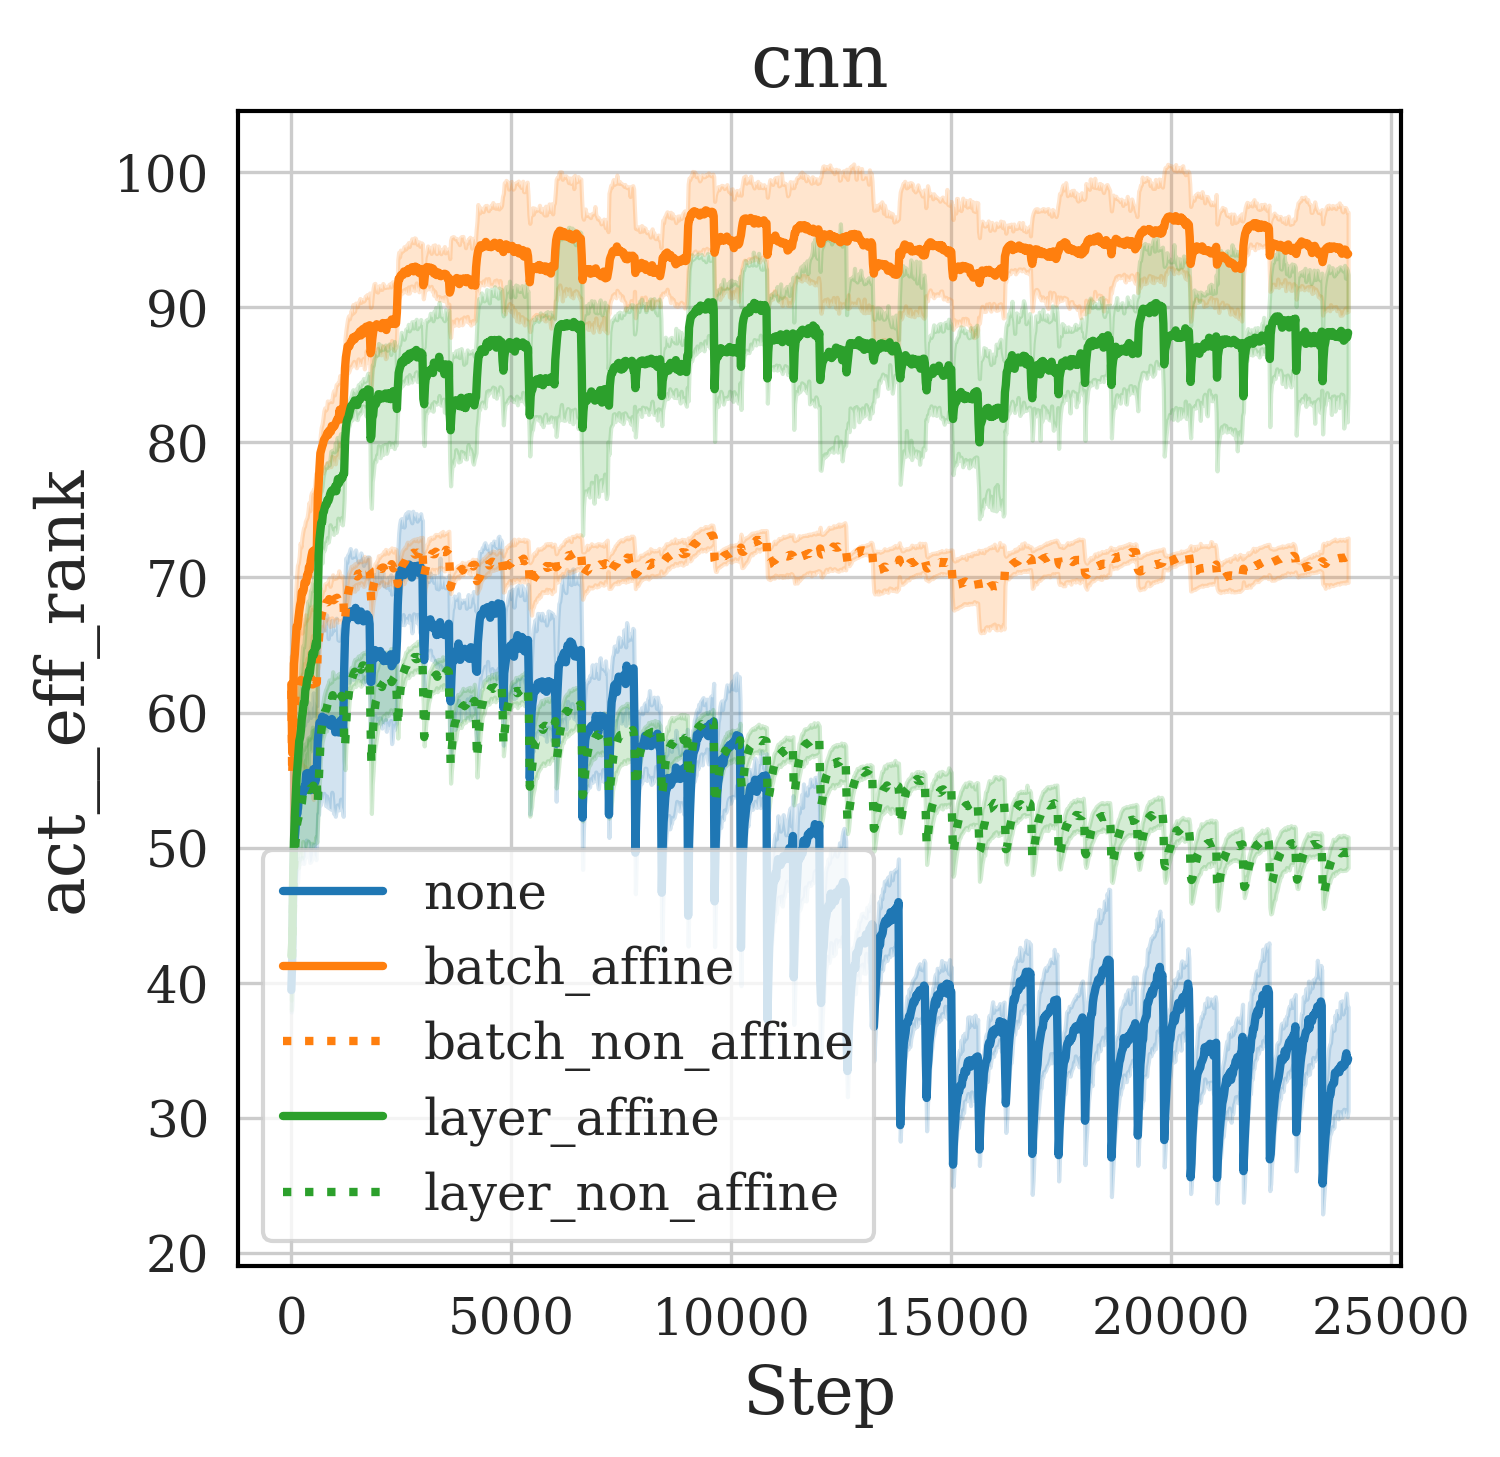
\includegraphics[width=0.24\linewidth]{cnn_rankandnorm.png}
    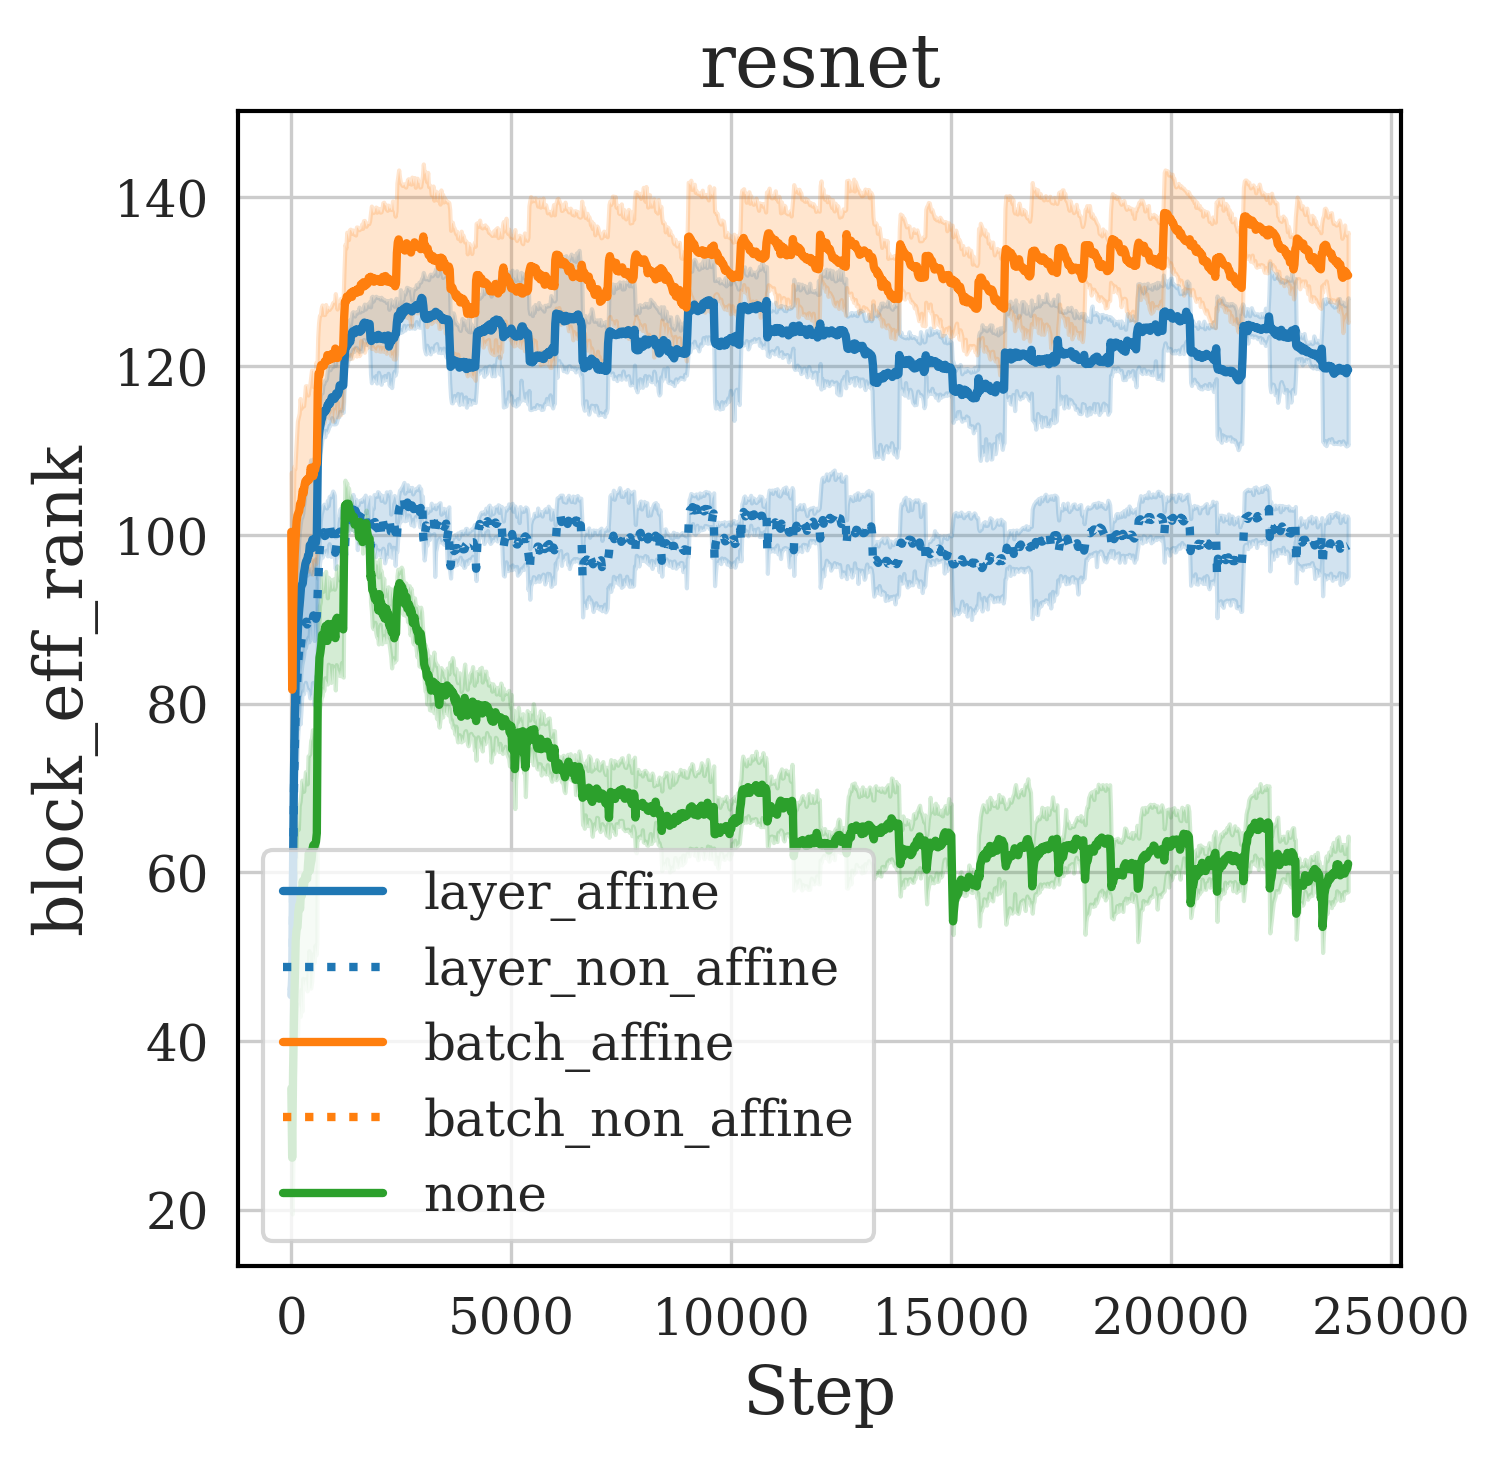
\includegraphics[width=0.24\linewidth]{resnet_rankandnorm.png} % Two resnet figs, combined to one idea
    % 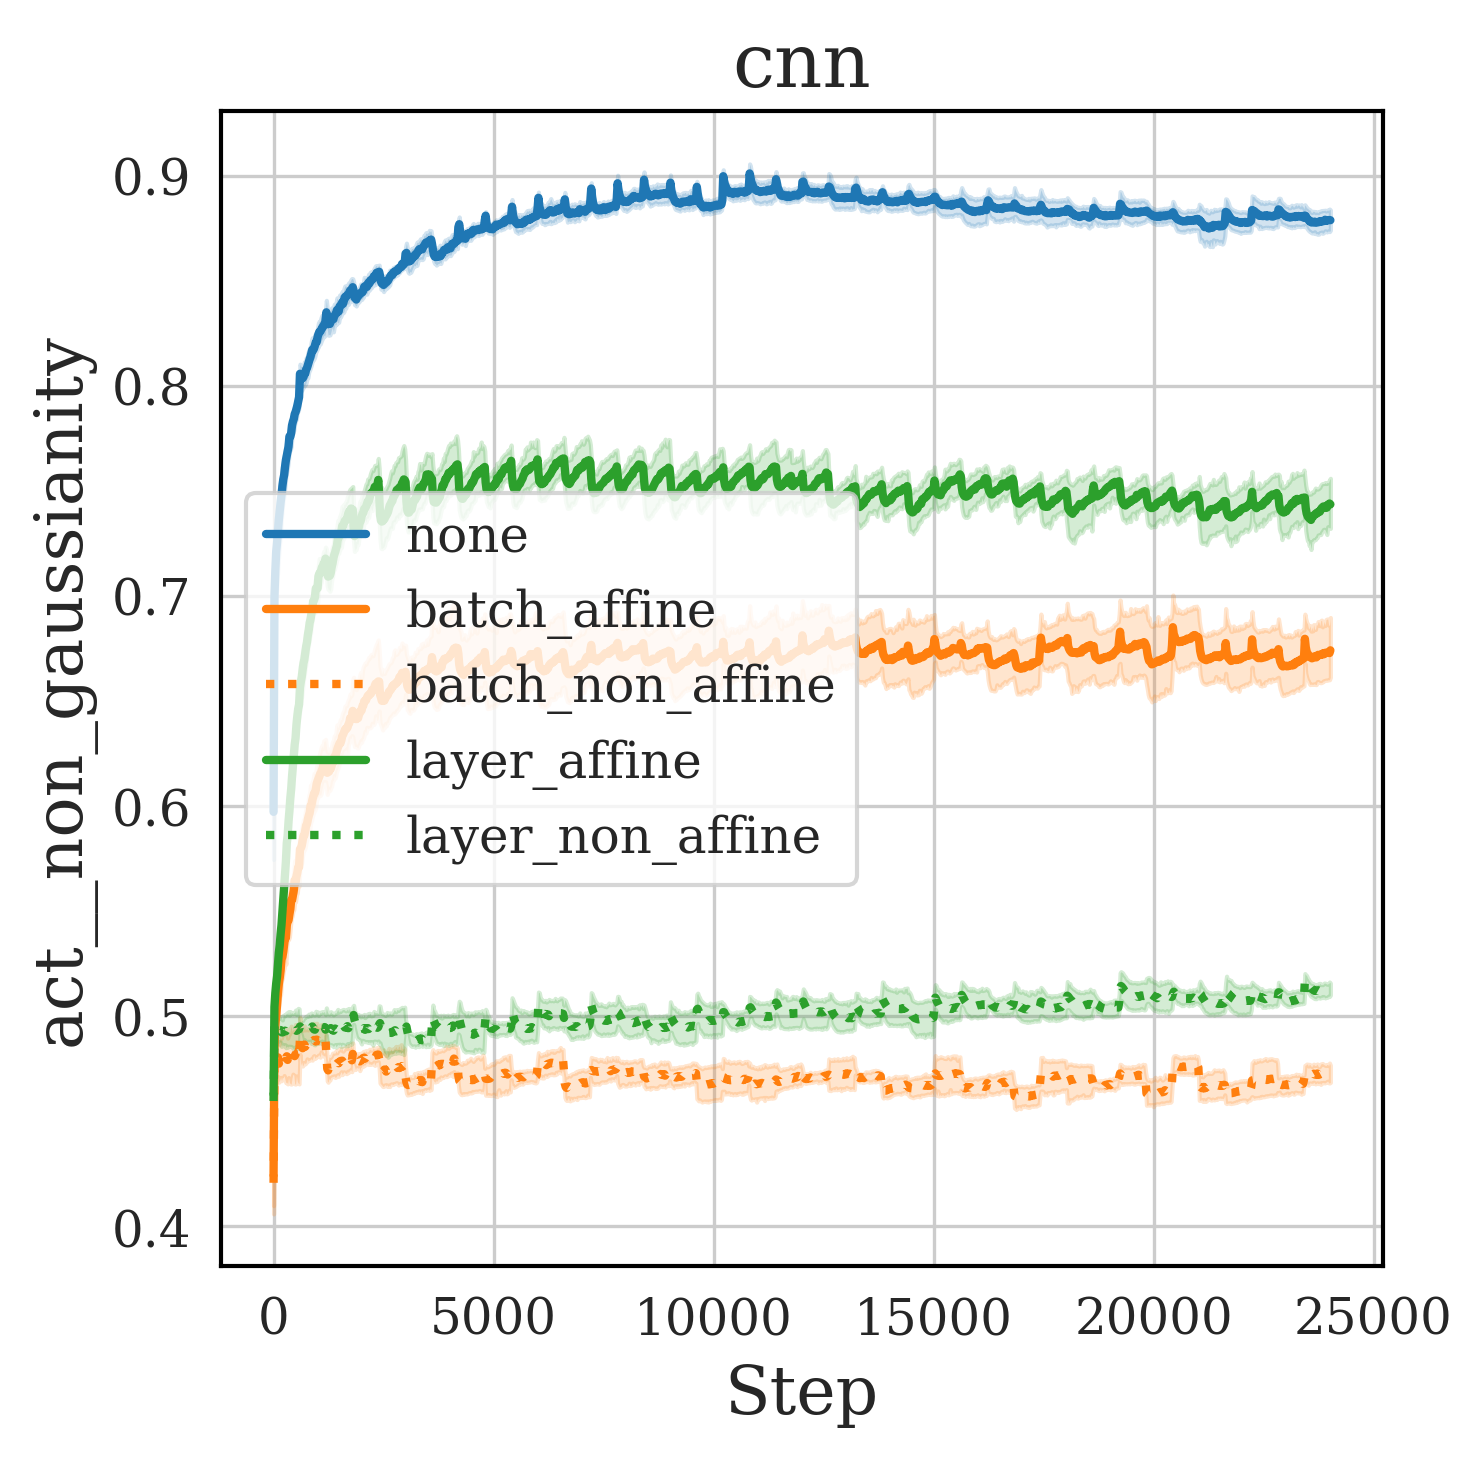
\includegraphics[width=0.24\linewidth]{cnn_nonGaussnorm.png} % Gaussianity for CNN
    % 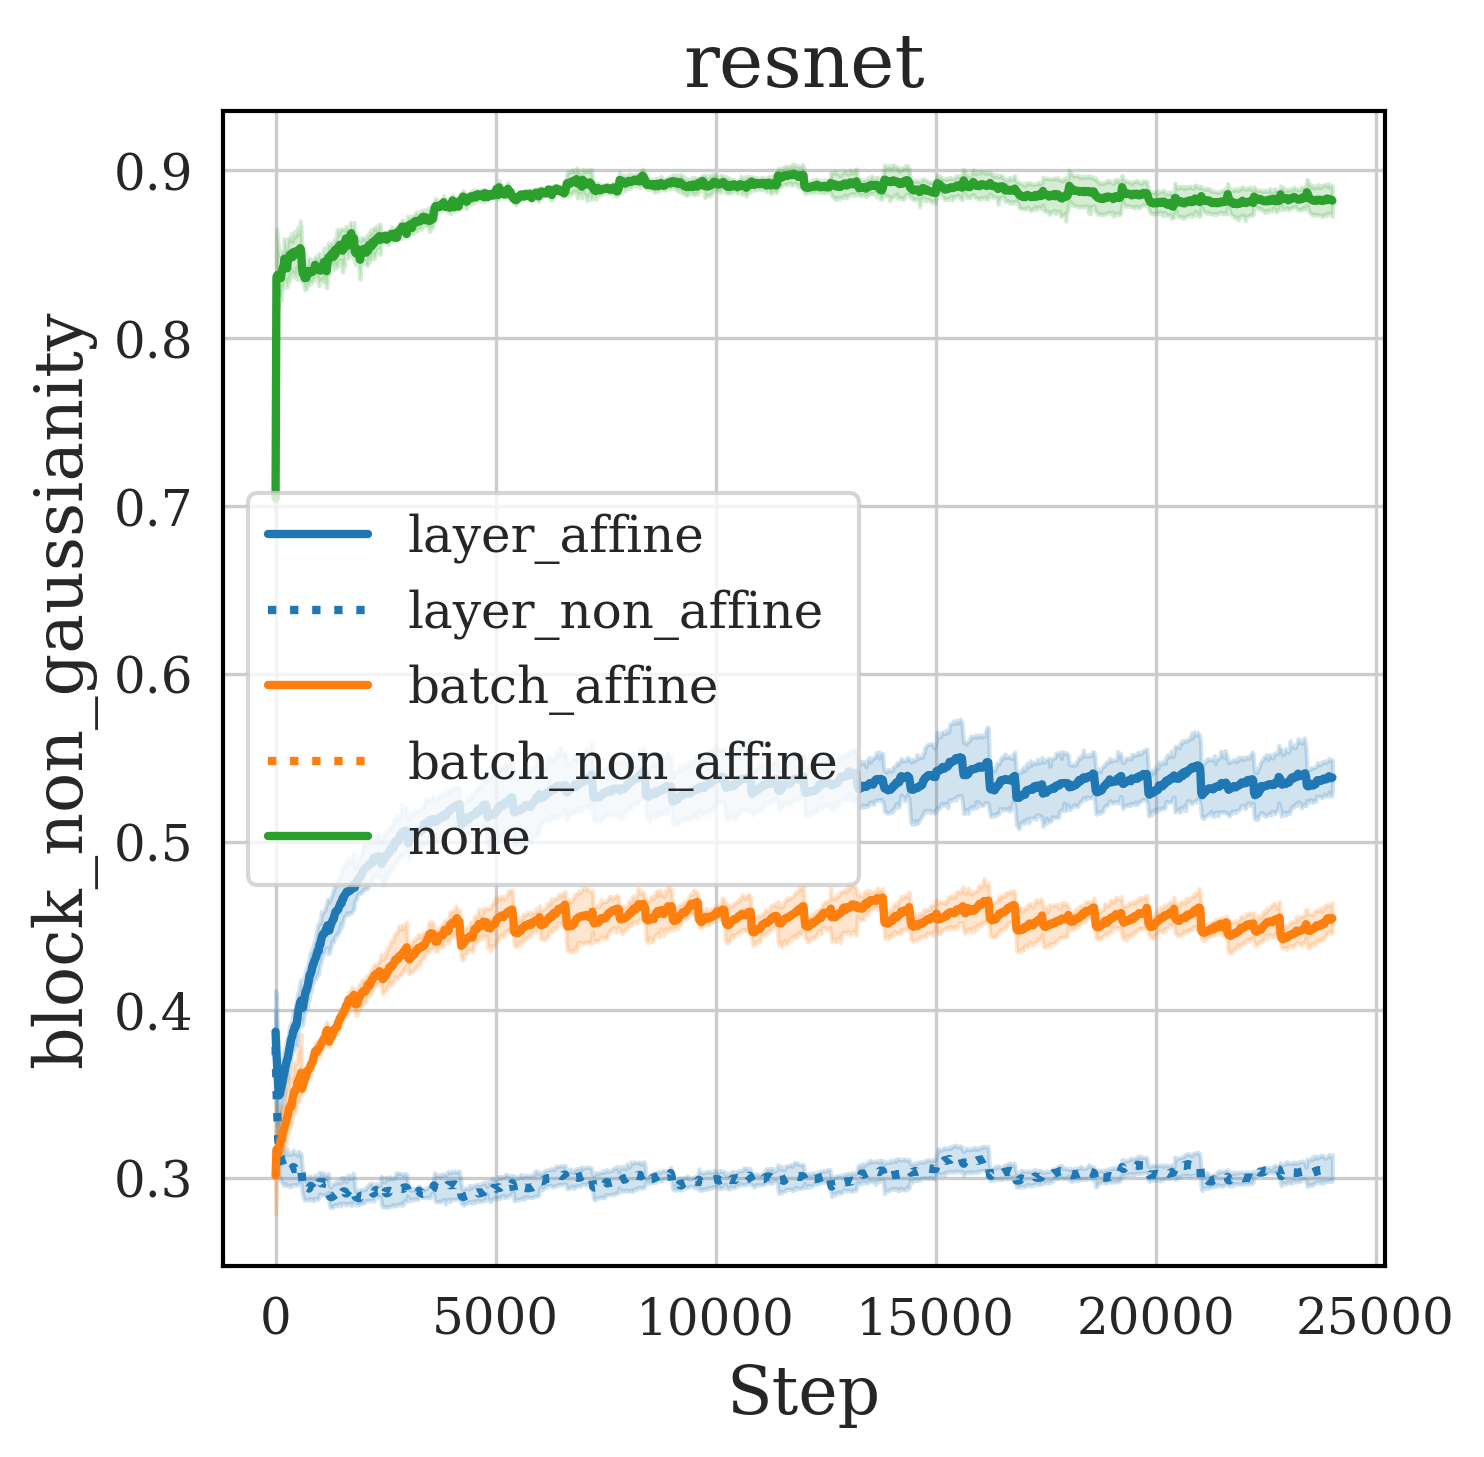
\includegraphics[width=0.24\linewidth]{resnet_nonGaussnorm.png} % Gaussianity for ResNet
    % 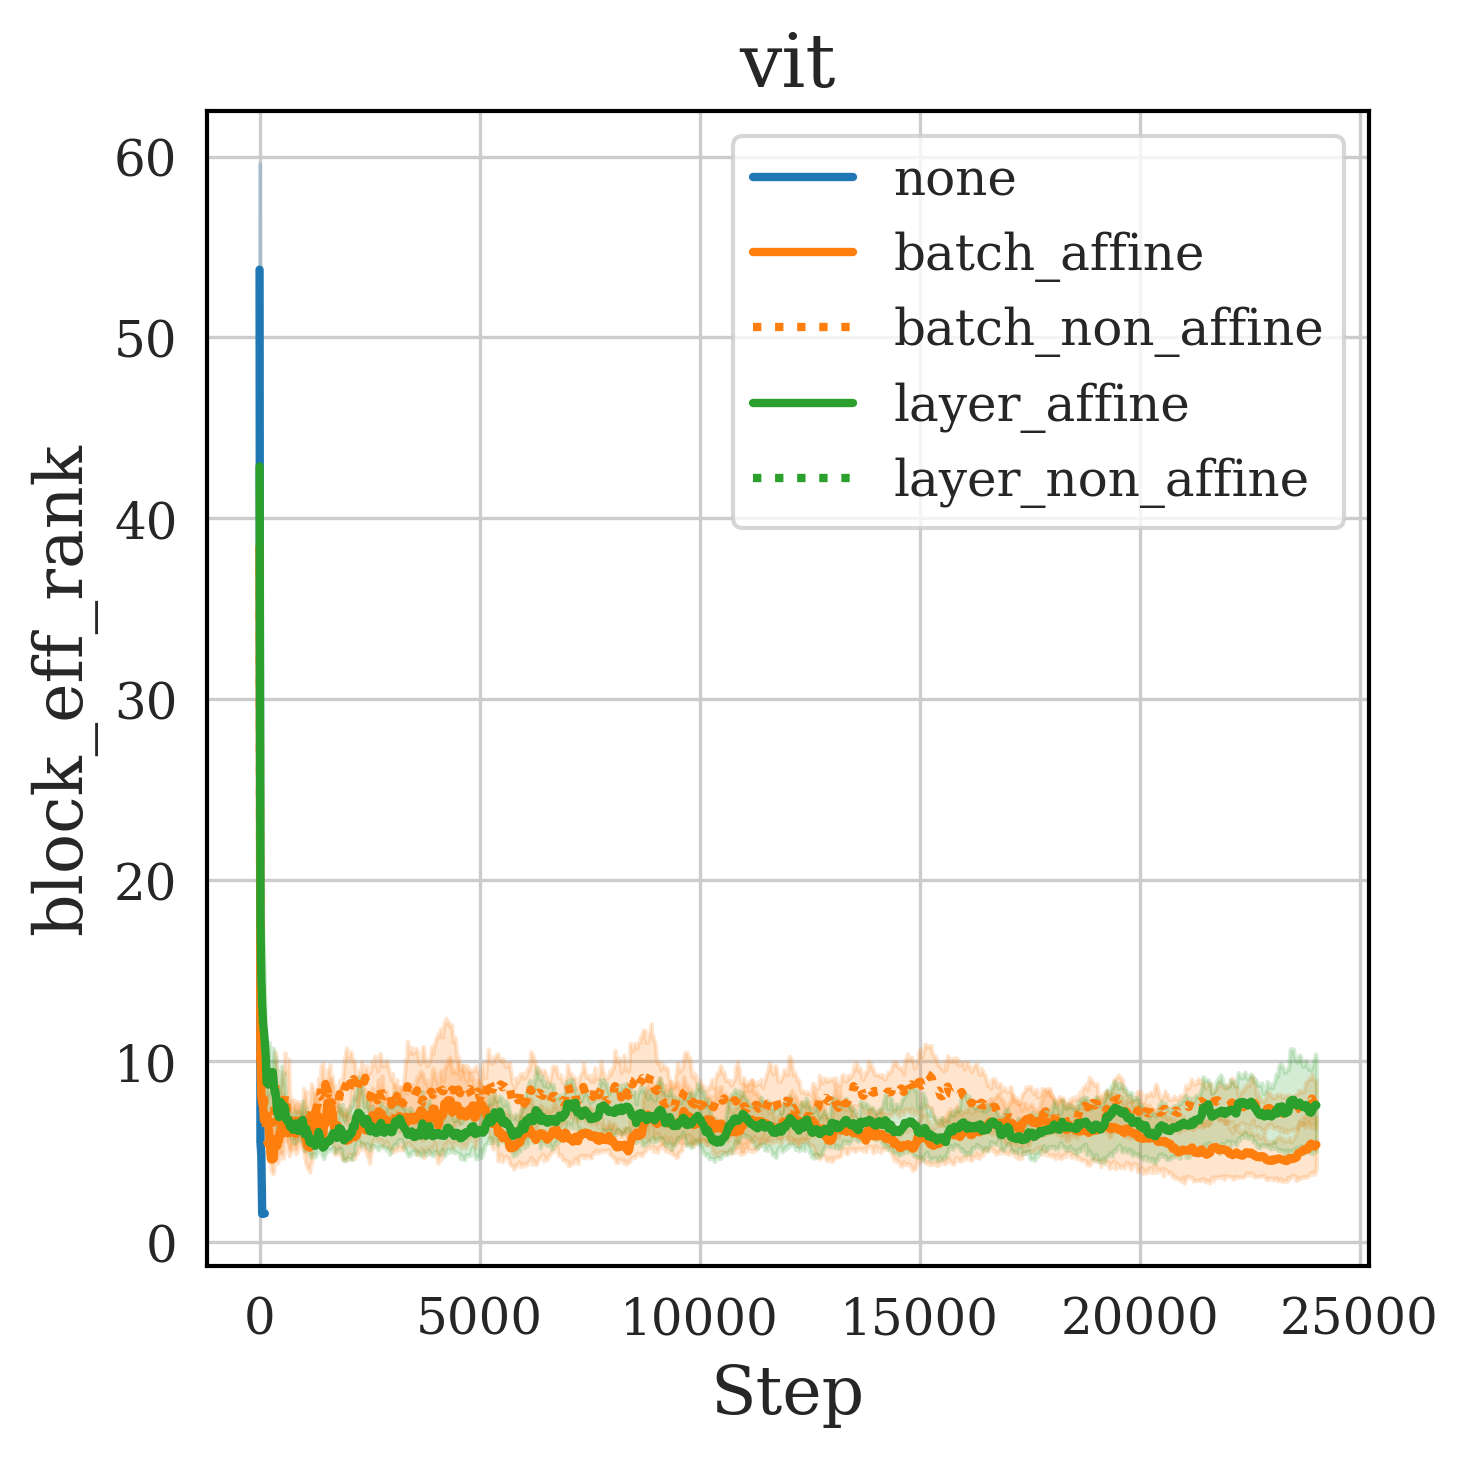
\includegraphics[width=0.24\linewidth]{vit_rankandnorm.png} % ViT rank and norm
    % 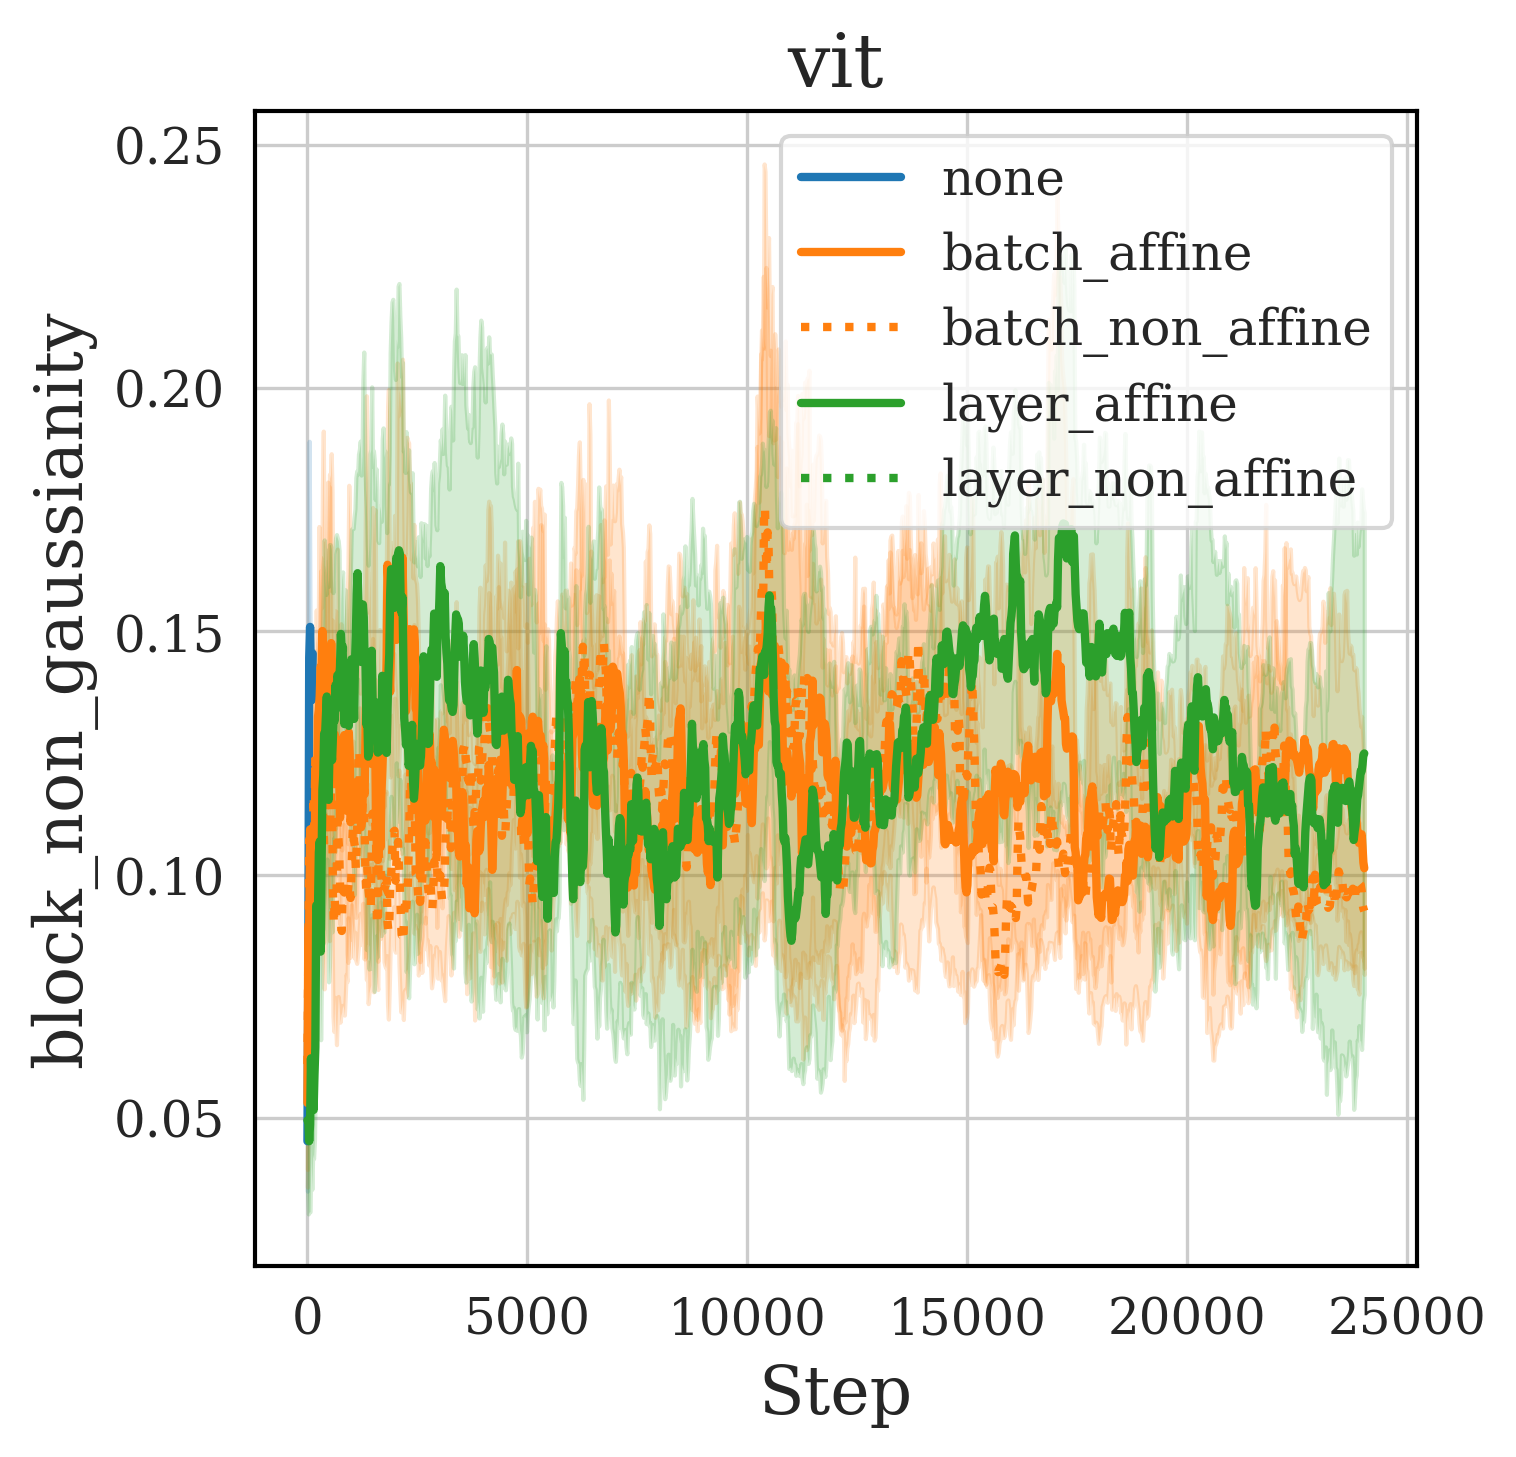
\includegraphics[width=0.24\linewidth]{vit_nonGaussnorm.png} % Gaussianity for ViT
    \caption{(Placeholder figures consolidated) Effect of normalization (e.g., None, Batch Norm, Layer Norm) on effective rank and non-Gaussianity of activations across various architectures (MLP, CNN, ResNet). Dropout is 0 unless specified. Normalization generally improves effective rank and can influence the distribution of activations. (Warning: Original caption noted color meanings may vary across architectures).}
    \label{fig:norm-rank-nG}
\end{figure}

\paragraph{Stochasticity and Regularization:}
Techniques that introduce stochasticity or prevent co-adaptation can also help maintain diversity.
\begin{itemize}
    \item \textbf{Dropout} \citep{srivastava2014dropout} randomly deactivates neurons during training. This prevents complex co-adaptations and can disrupt the formation of cloned-unit manifolds (Proposition~\ref{prop:cloned}) by breaking symmetries. It helps maintain representational diversity and rank. Figure~\ref{fig:dropout-rank} (placeholder) illustrates Dropout's effect on effective rank.
    % Giulia's comment: "We need to remove dropout from here". However, user's notes and existing draft figures include it. 
    % Retaining for now, with a note that its role in CL can be complex (sometimes detrimental if it discards learned info too aggressively).
    % If this is definitively to be removed, the text and figure reference should be deleted by the authors.
\end{itemize}

\begin{figure}[h!]
    \centering
    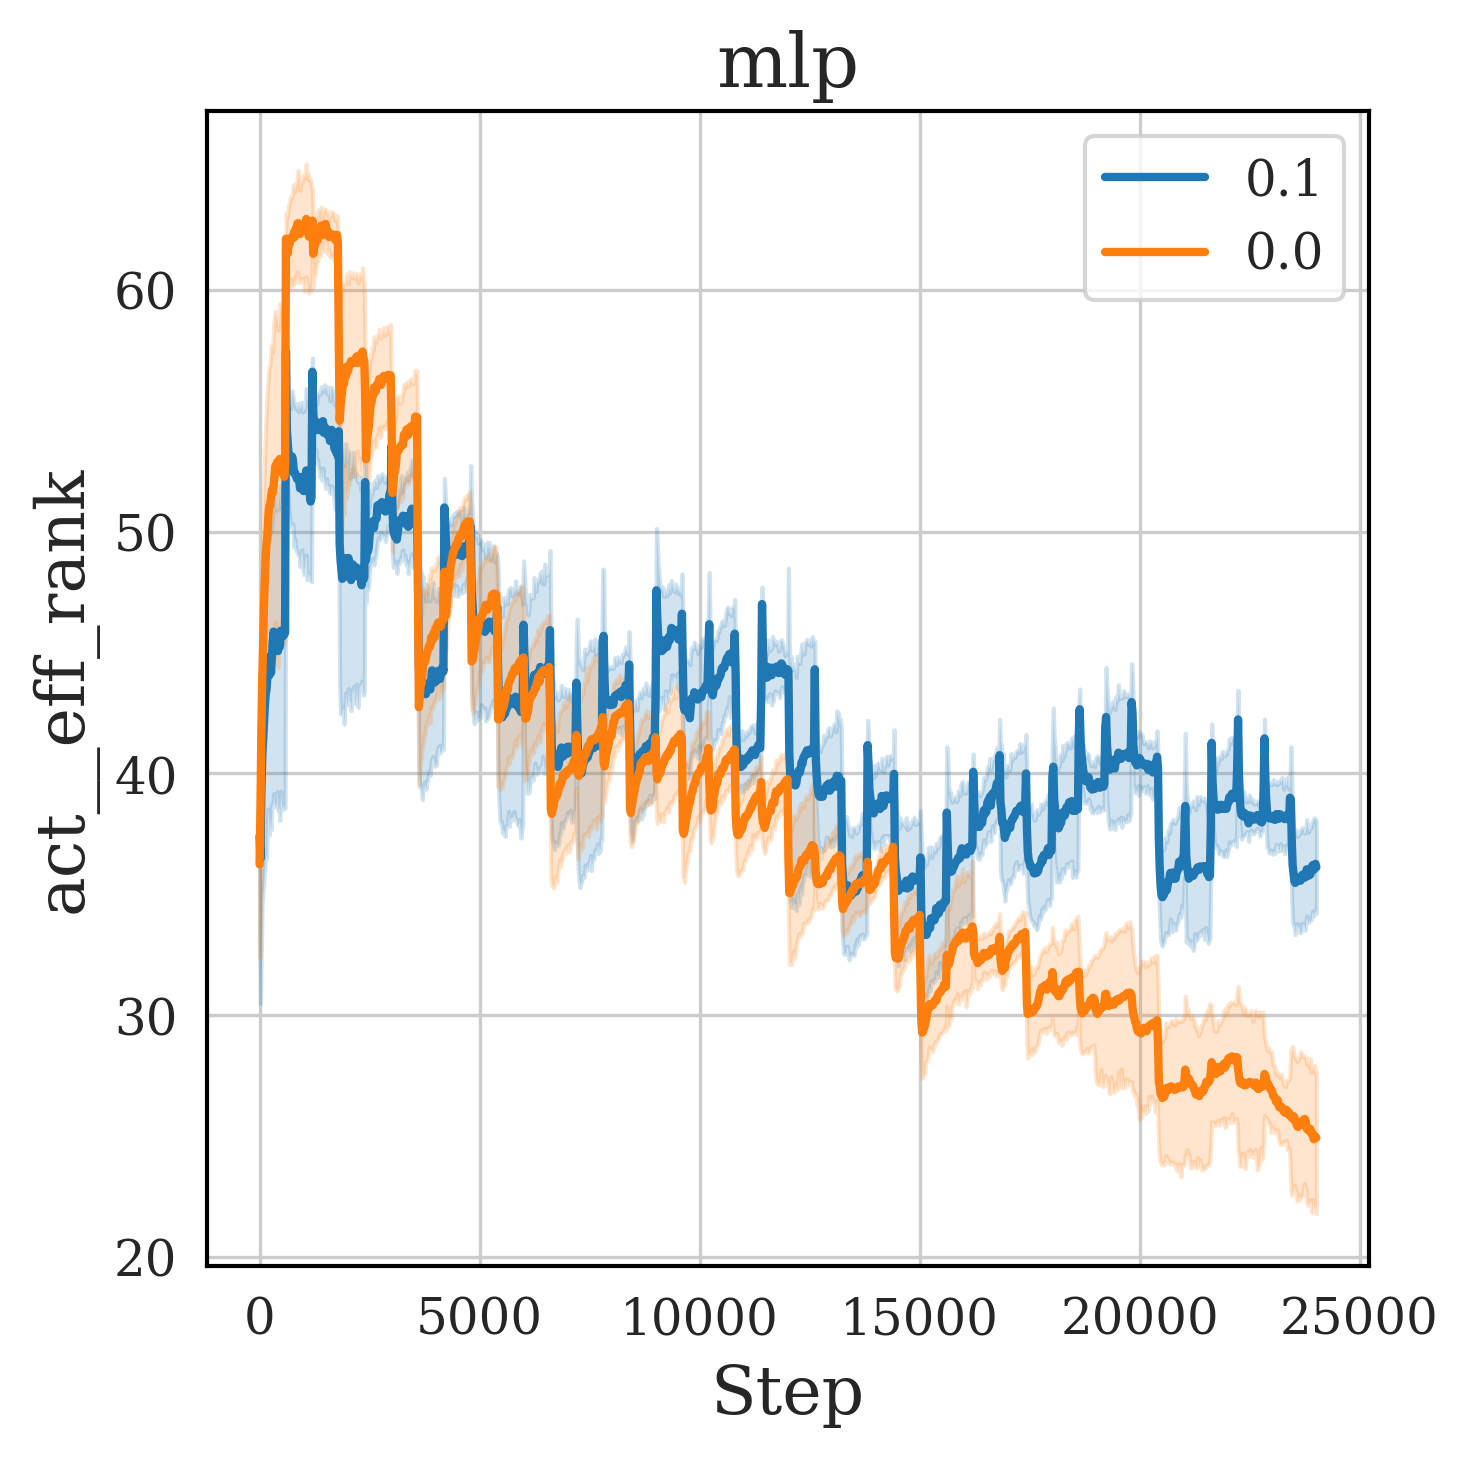
\includegraphics[width=0.24\linewidth]{mlp_rankanddropout.png}
    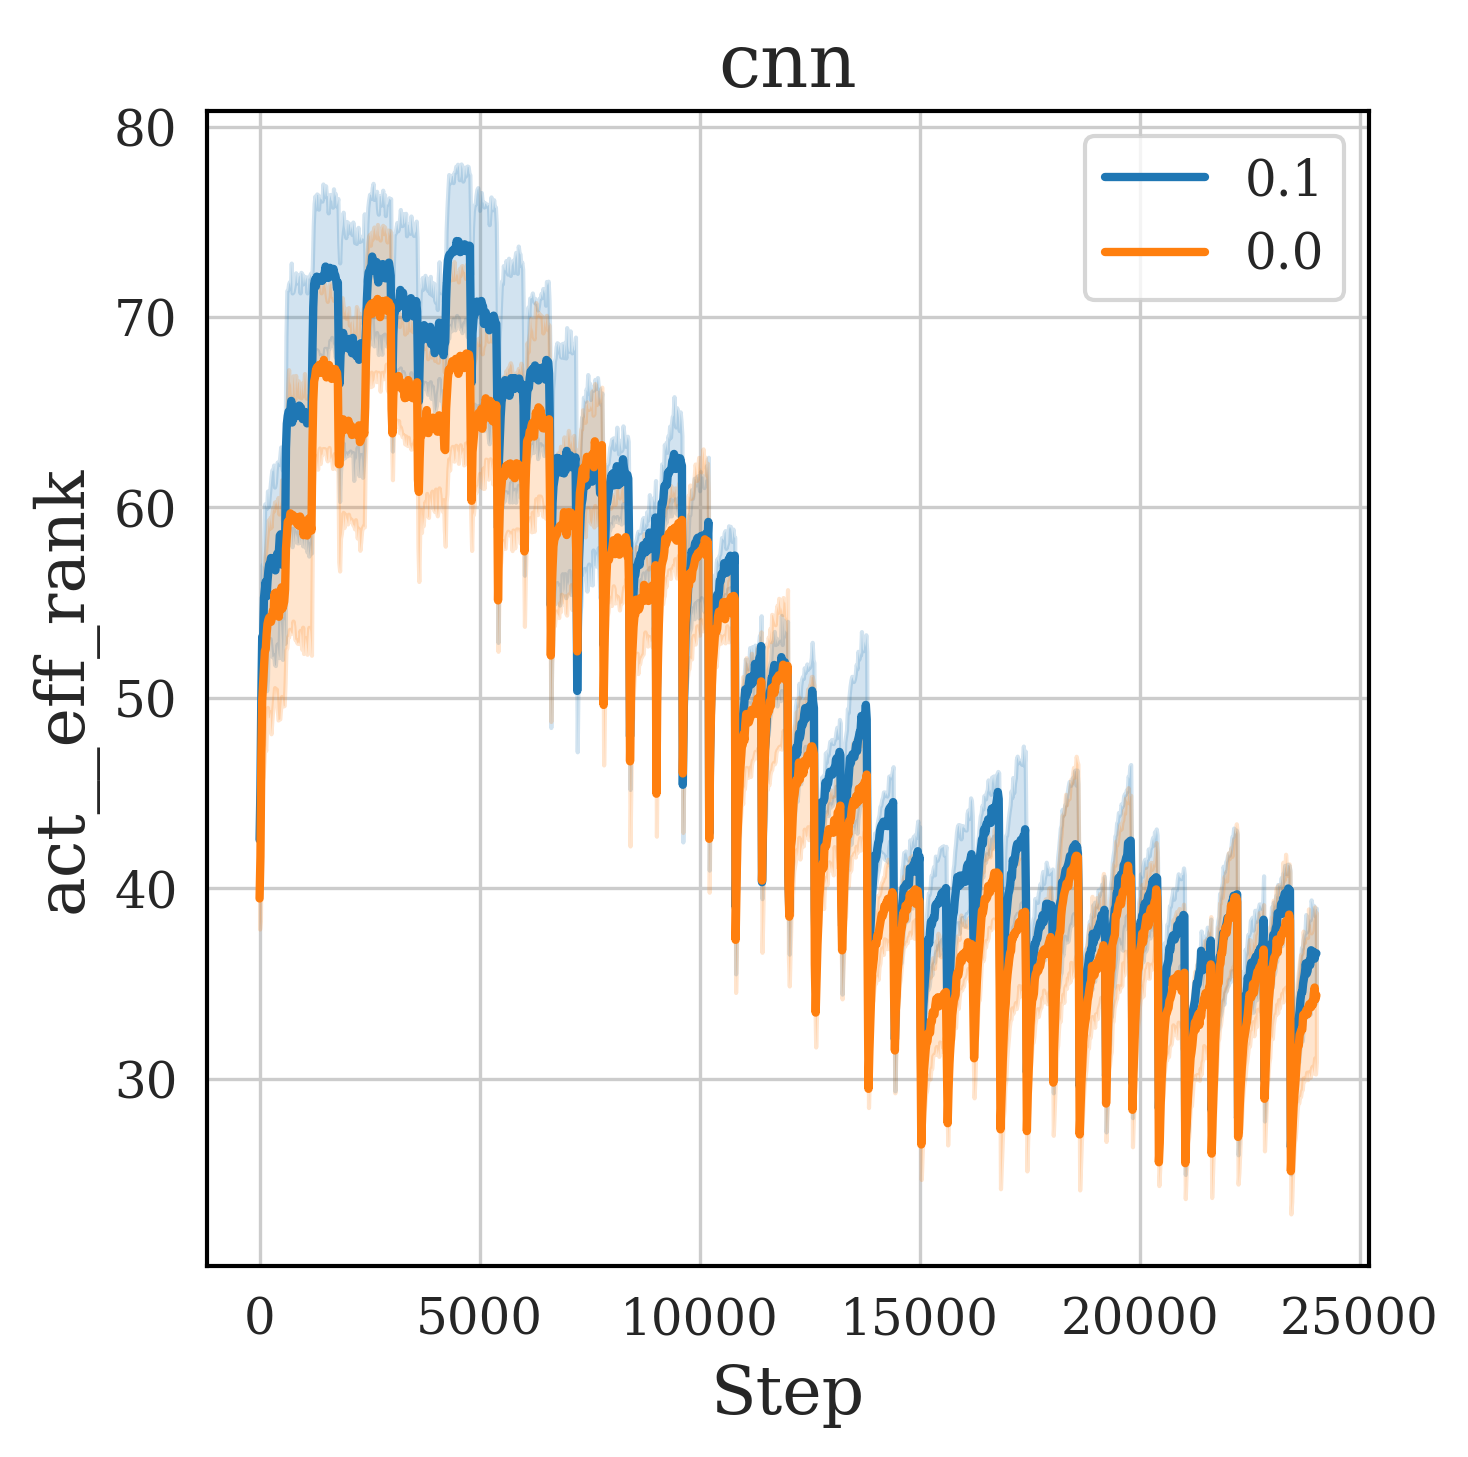
\includegraphics[width=0.24\linewidth]{cnn_rankanddropout.png}
    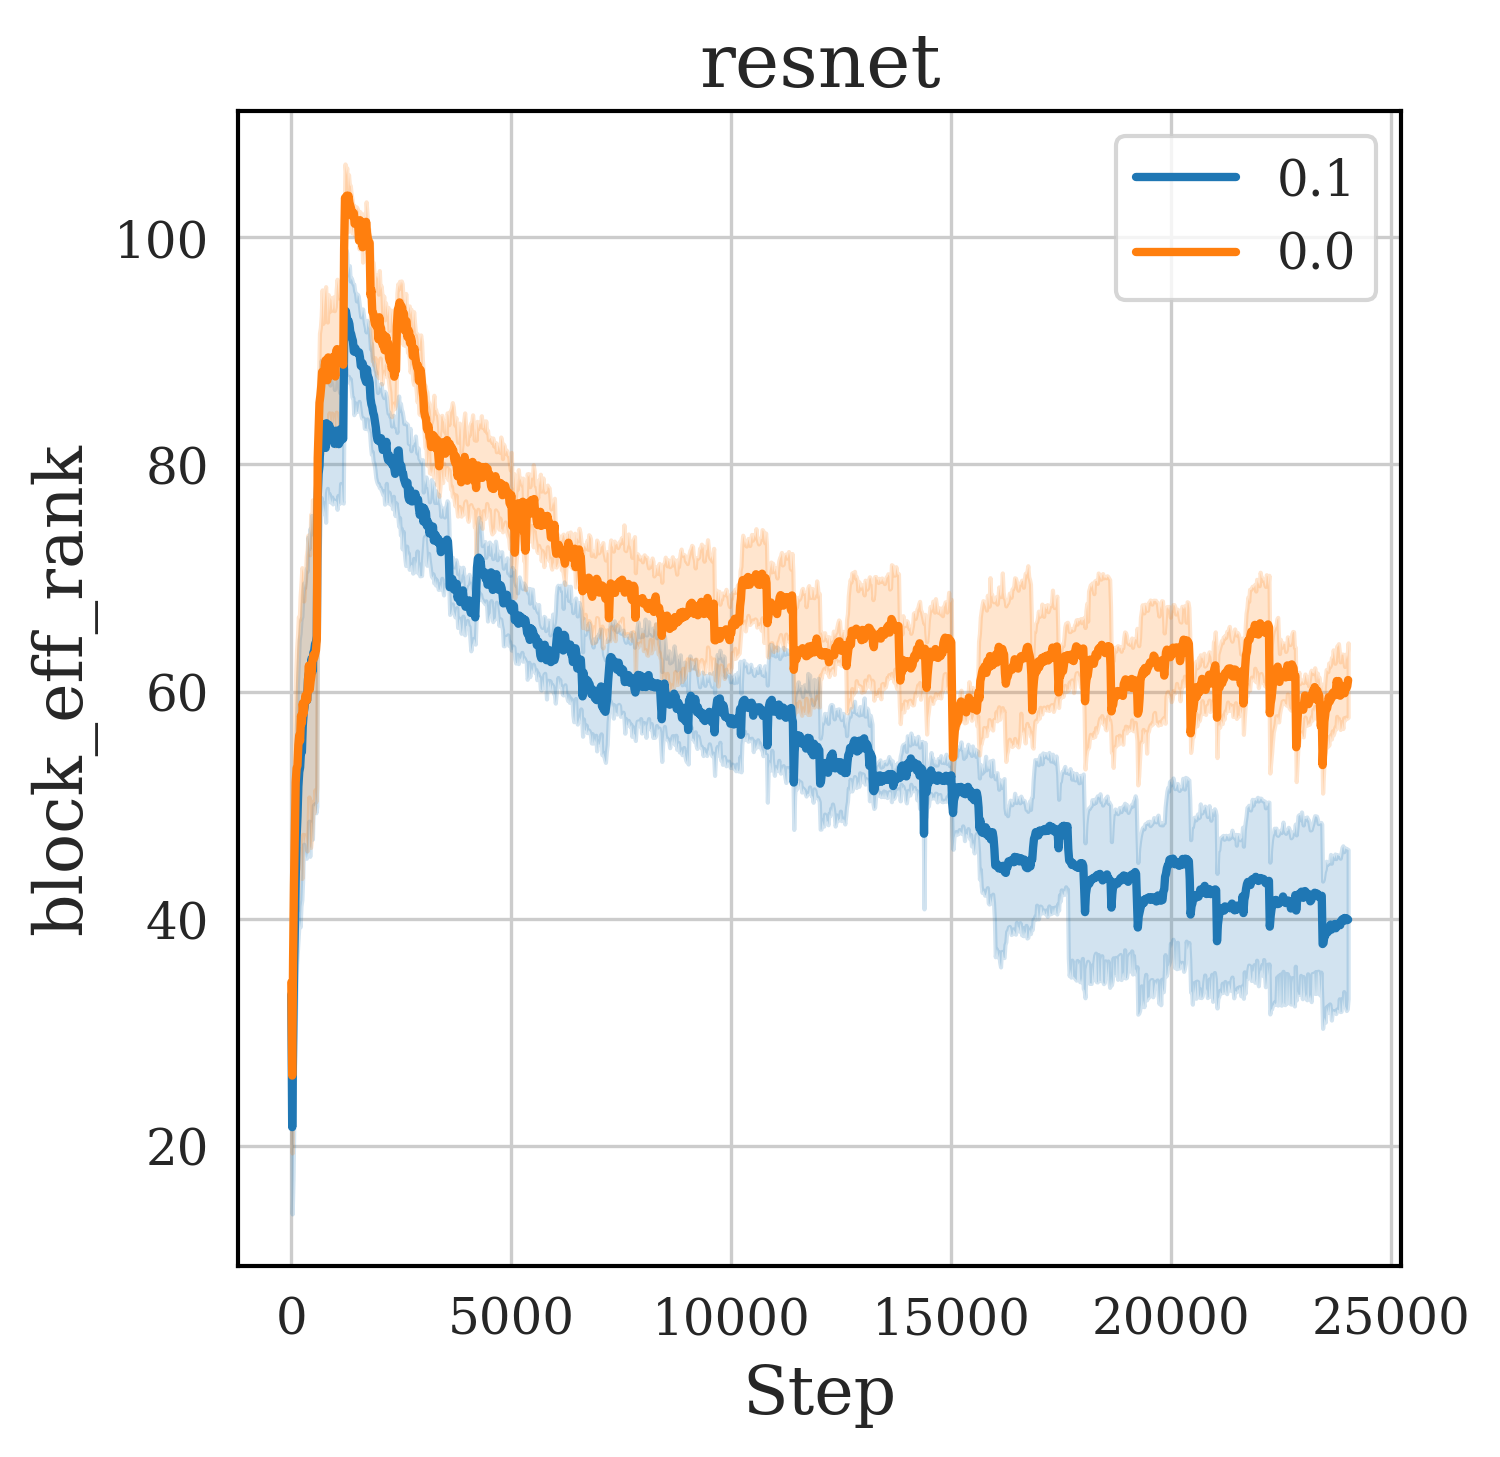
\includegraphics[width=0.24\linewidth]{resnet_rankanddropout.png}
    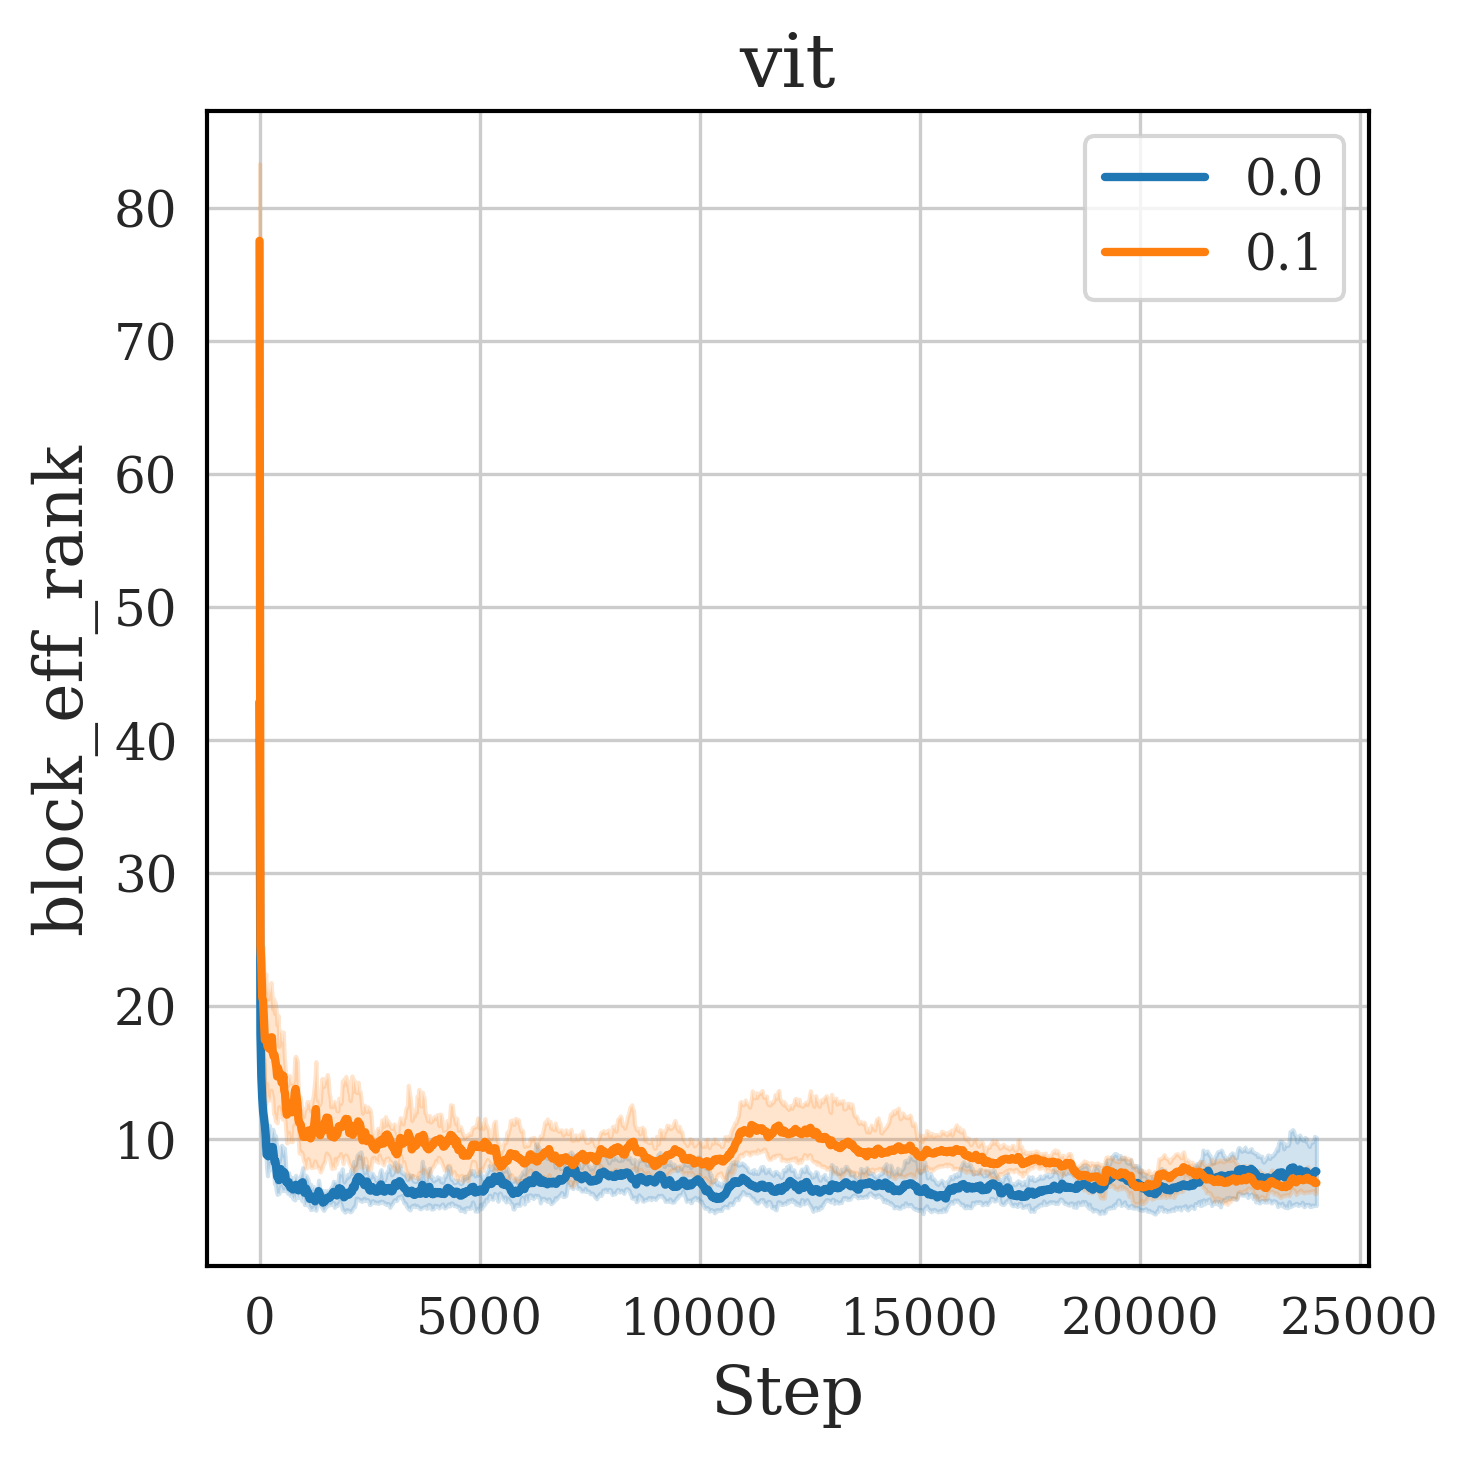
\includegraphics[width=0.24\linewidth]{vit_rankanddropout.png}
    \caption{(Placeholder figure) Effect of dropout on Effective Rank across different architectures (MLP, CNN, ResNet, ViT). No normalization applied, except LayerNorm on ViT as specified in the original draft.}
    \label{fig:dropout-rank}
\end{figure}

\subsection{Escaping an LoP Manifold}
If a network's parameters $\theta(t)$ have already converged to a stable LoP manifold $\mathcal{M}$, standard gradient descent will not facilitate escape. However, perturbations or noise injection might allow the trajectory to leave $\mathcal{M}$, particularly if the manifold is not stable in all normal directions.

\begin{corollary}[Perturbation Dynamics for Escaping LoP Manifolds]
\label{cor:perturb}
Suppose parameters are at $\theta_0 \in \mathcal{M}$. Consider a small perturbation $\varepsilon v$ in a direction $v$ normal to $\mathcal{M}$ at $\theta_0$ (i.e., $v \in N_{\theta_0}\mathcal{M}$, $\|v\|=1$). The state after perturbation is $\theta(0)=\theta_0+\varepsilon v$, for $\varepsilon \ll 1$.
The initial rate of change of the squared distance from $\mathcal{M}$ under gradient flow (Eq.~\ref{eq:grad_flow}) can be approximated. Let $\mathrm{dist}^2(\theta, \mathcal{M})$ be the squared Euclidean distance from $\theta$ to the closest point on $\mathcal{M}$. Then,
\[
\frac{d}{dt}\left.\mathrm{dist}^2(\theta(t),\mathcal{M})\right|_{t=0} \approx -2\varepsilon^2\,v^\top\nabla_\theta^2\Loss(\theta_0)v + O(\varepsilon^3).
\]
This approximation relies on a Taylor expansion of $\nabla_\theta \Loss(\theta(0))$ around $\theta_0$ and the fact that $v^\top \nabla_\theta \Loss(\theta_0) = 0$ since $\nabla_\theta \Loss(\theta_0)$ is tangent to $\mathcal{M}$ and $v$ is normal.
The distance from the manifold will initially increase (plasticity potentially recovered) if and only if there exists a normal direction $v$ with negative curvature, $v^\top\nabla_\theta^2\Loss(\theta_0)v < 0$.
\end{corollary}
% \keivan{I think it is good to mention "according to the taylor expansion principle the above holds", or even give a little more explanation in appendix to make the reviewers work easier. It was not obvious for me first time specially confusing $\theta(0)$ and $\theta_0$}
% Added a brief explanation for the approximation.

This corollary highlights that escape via gradient descent post-perturbation depends on the geometry of the loss landscape normal to $\mathcal{M}$.
\begin{itemize}
    \item If $\mathcal{M}$ is \textbf{stable} (positive curvature in all normal directions, Eq.~\ref{eq:stable}), noise alone followed by gradient descent won't lead to escape.
    \item If $\mathcal{M}$ is of \textbf{saddle type} (Eq.~\ref{eq:saddle}), perturbations along directions of negative curvature can initiate escape trajectories.
    \item If $\mathcal{M}$ is \textbf{unstable} (Eq.~\ref{eq:unstable}), any generic perturbation will likely lead to escape.
\end{itemize}
This explains why techniques involving noise injection (e.g., noisy SGD) or periodic re-diversification (e.g., continual backpropagation \citep{dohare2024loss}, which reintroduces randomness) can sometimes restore plasticity. They might push parameters off $\mathcal{M}$ into regions where gradient flow leads away from it.

Figures \ref{fig:CBP-scale-rank-main} and \ref{fig:CBP-dup-frac-main} (placeholders) compare standard backpropagation (BP) with Continual Backpropagation (CBP), suggesting CBP can mitigate the emergence of low-rank structures and duplicated units, thereby preserving plasticity.

\begin{figure}[h!]
    \centering
    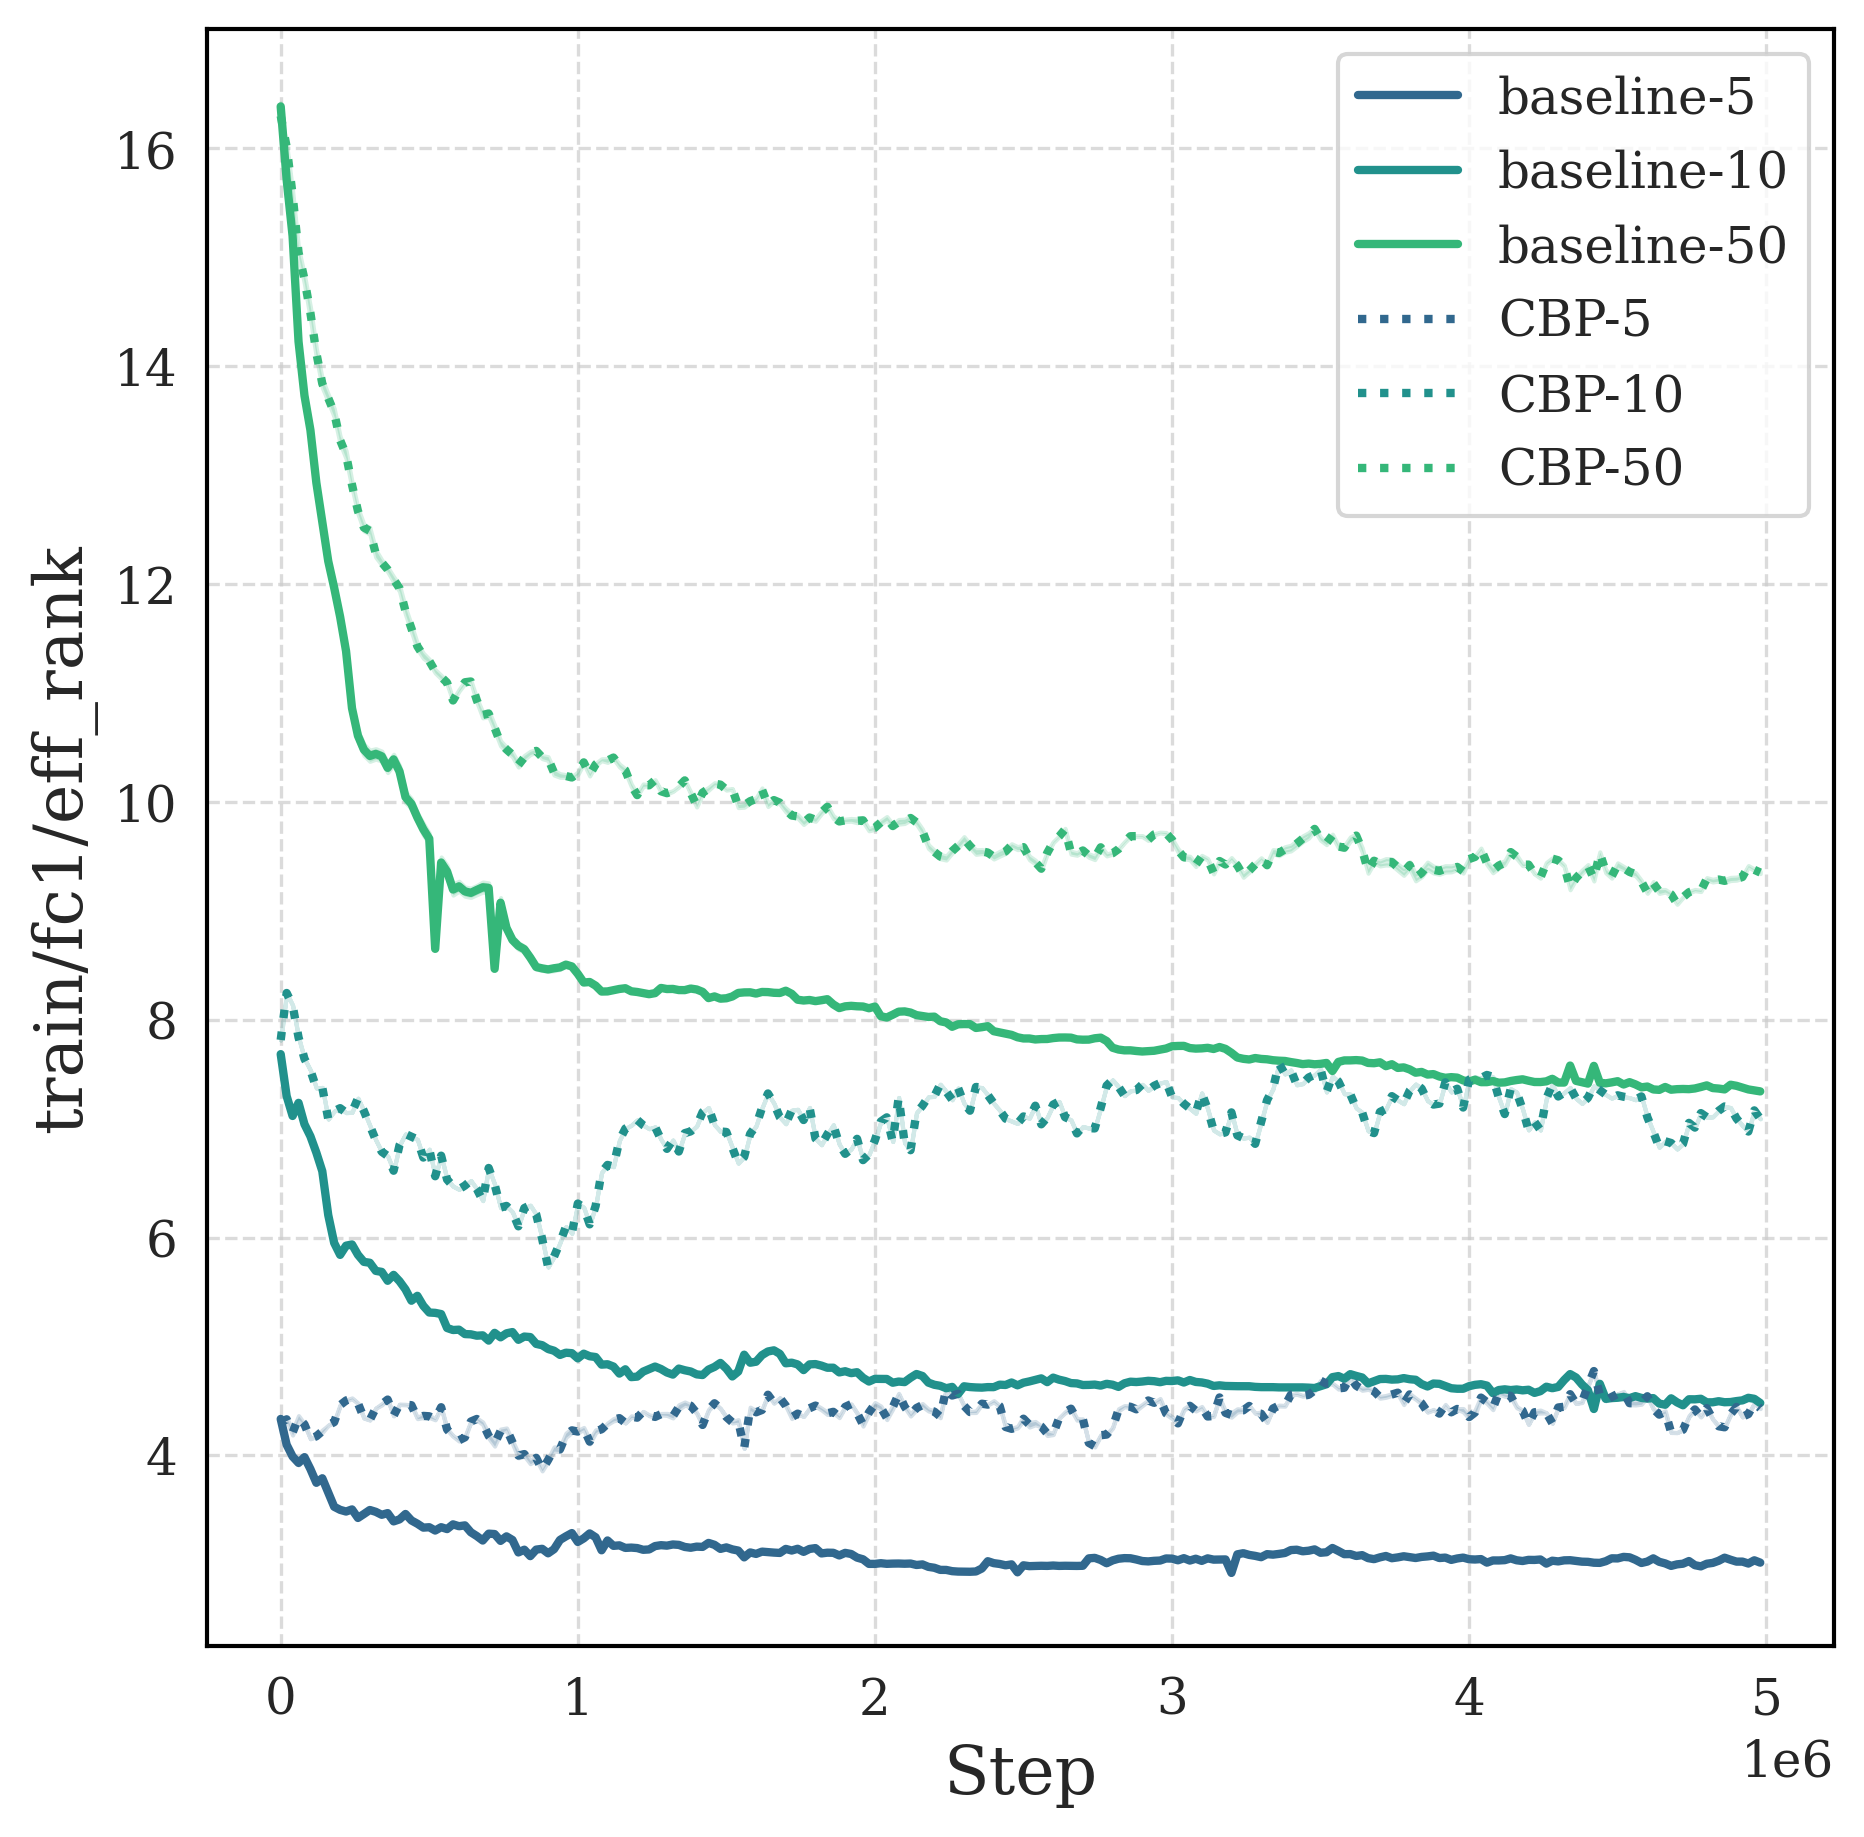
\includegraphics[width=0.33\linewidth]{CBP-scale-rank.png}
    \caption{(Placeholder figure) Bit Flipping experiment. Low-rank structures (e.g., measured by effective rank or singular value decay of activations) emerge during training with standard BP but are less pronounced with CBP, suggesting CBP helps maintain feature diversity.}
    \label{fig:CBP-scale-rank-main}
\end{figure}

\begin{figure}[h!]
    \centering
    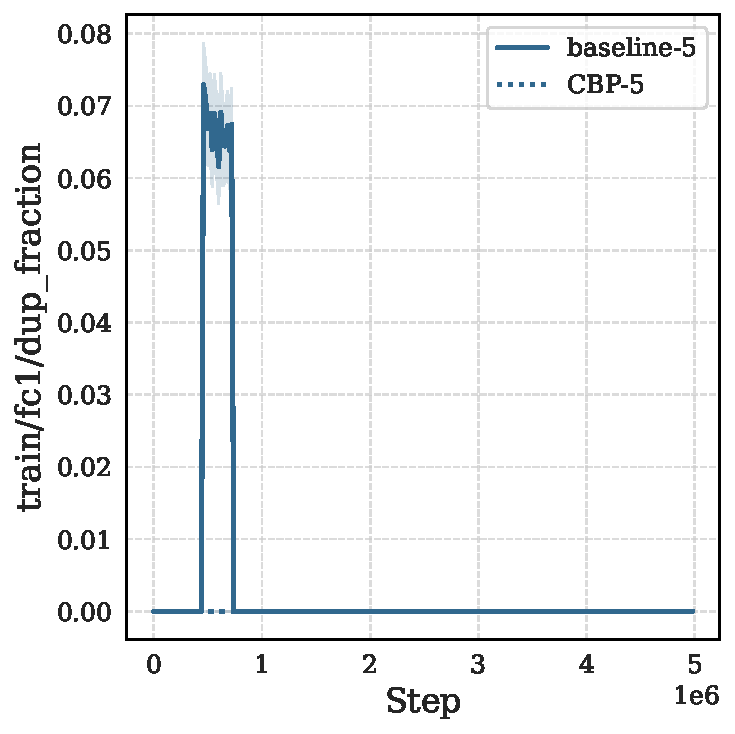
\includegraphics[width=0.23\linewidth]{CBP-dup_fraction-5.pdf}
    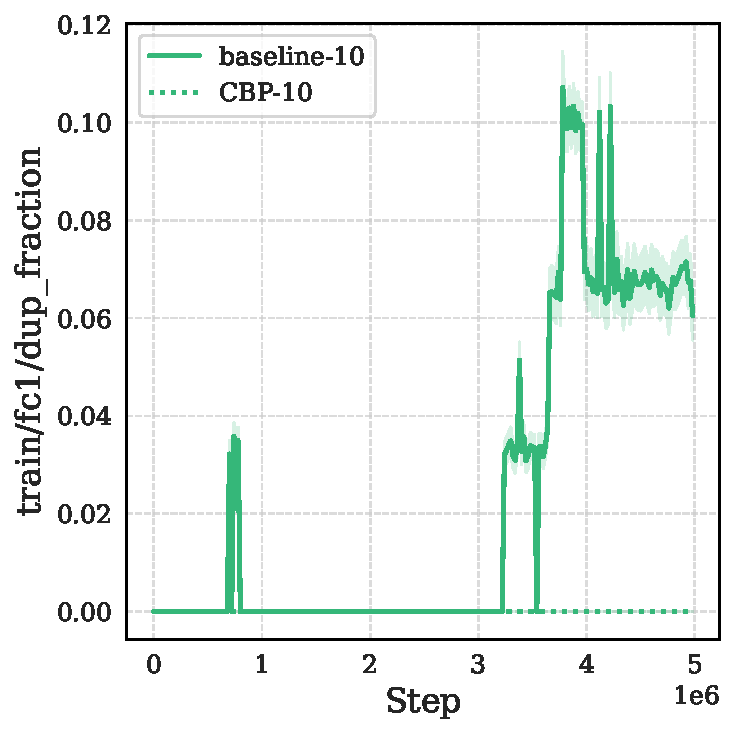
\includegraphics[width=0.23\linewidth]{CBP-dup_fraction-10.pdf}
    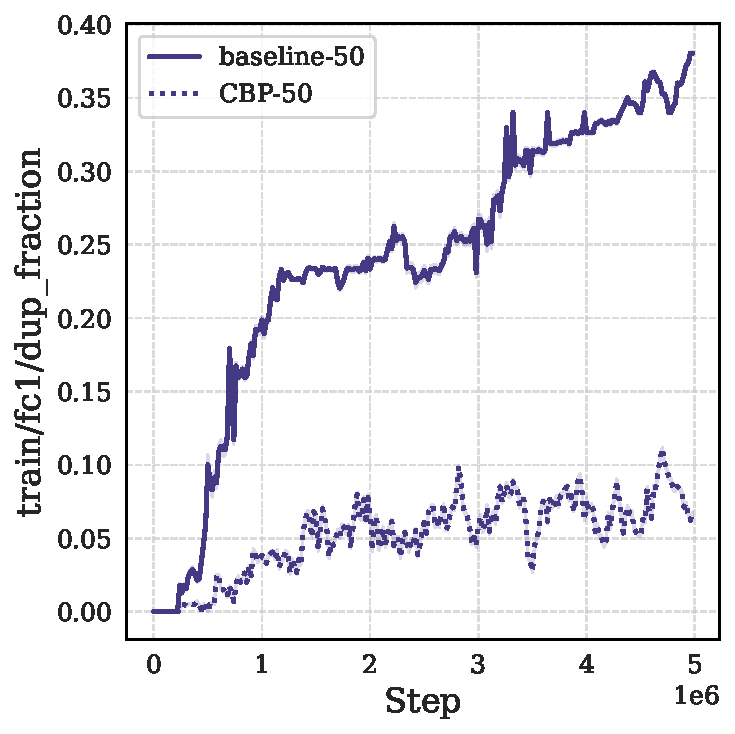
\includegraphics[width=0.23\linewidth]{CBP-dup_fraction-50.pdf}
    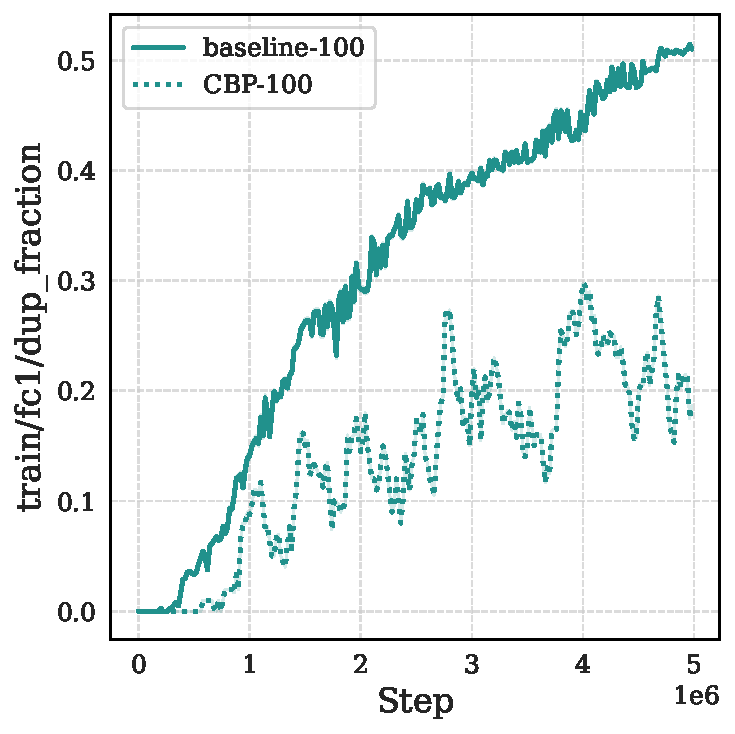
\includegraphics[width=0.23\linewidth]{CBP-dup_fraction-100.pdf}
    \caption{(Placeholder figure) Bit Flipping experiment. Duplicated unit fractions at different scales/layers (indicated by 5, 10, 50, 100 in filenames, interpretation context dependent). Duplicated structures emerge more with BP than with CBP.}
    \label{fig:CBP-dup-frac-main}
\end{figure}

The final performance, as summarized in Figure~\ref{fig:mlp-config-finalperf} (placeholder), often depends significantly on choices like normalization and dropout, which influence the network's trajectory relative to LoP manifolds.

\begin{figure}[h!]
    \centering
    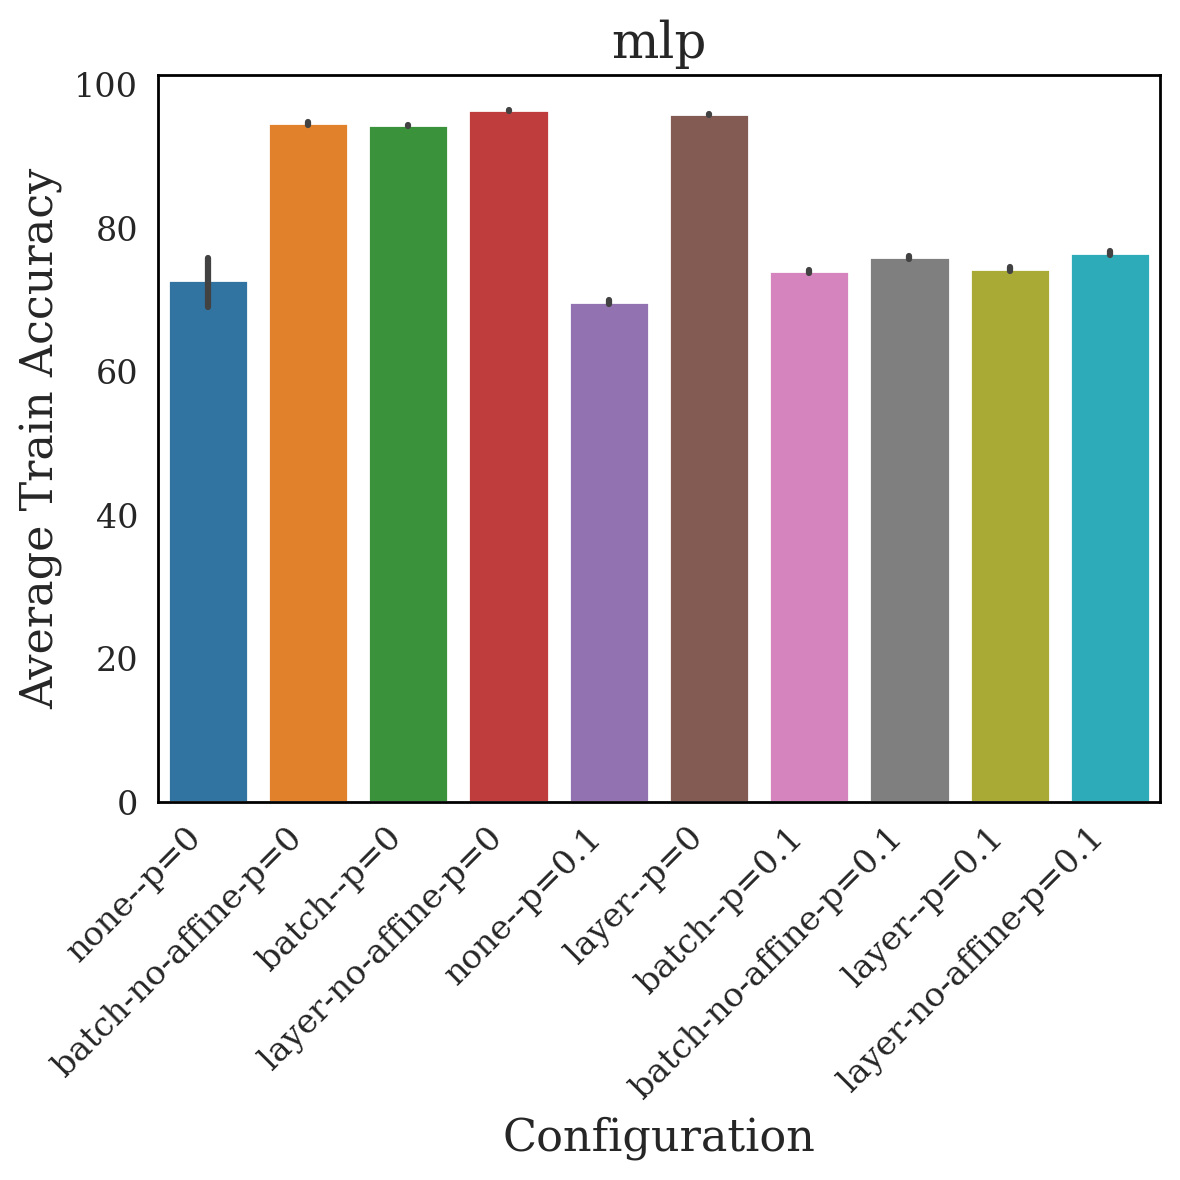
\includegraphics[width=0.3\linewidth]{mlp_config_finalperf.png}
    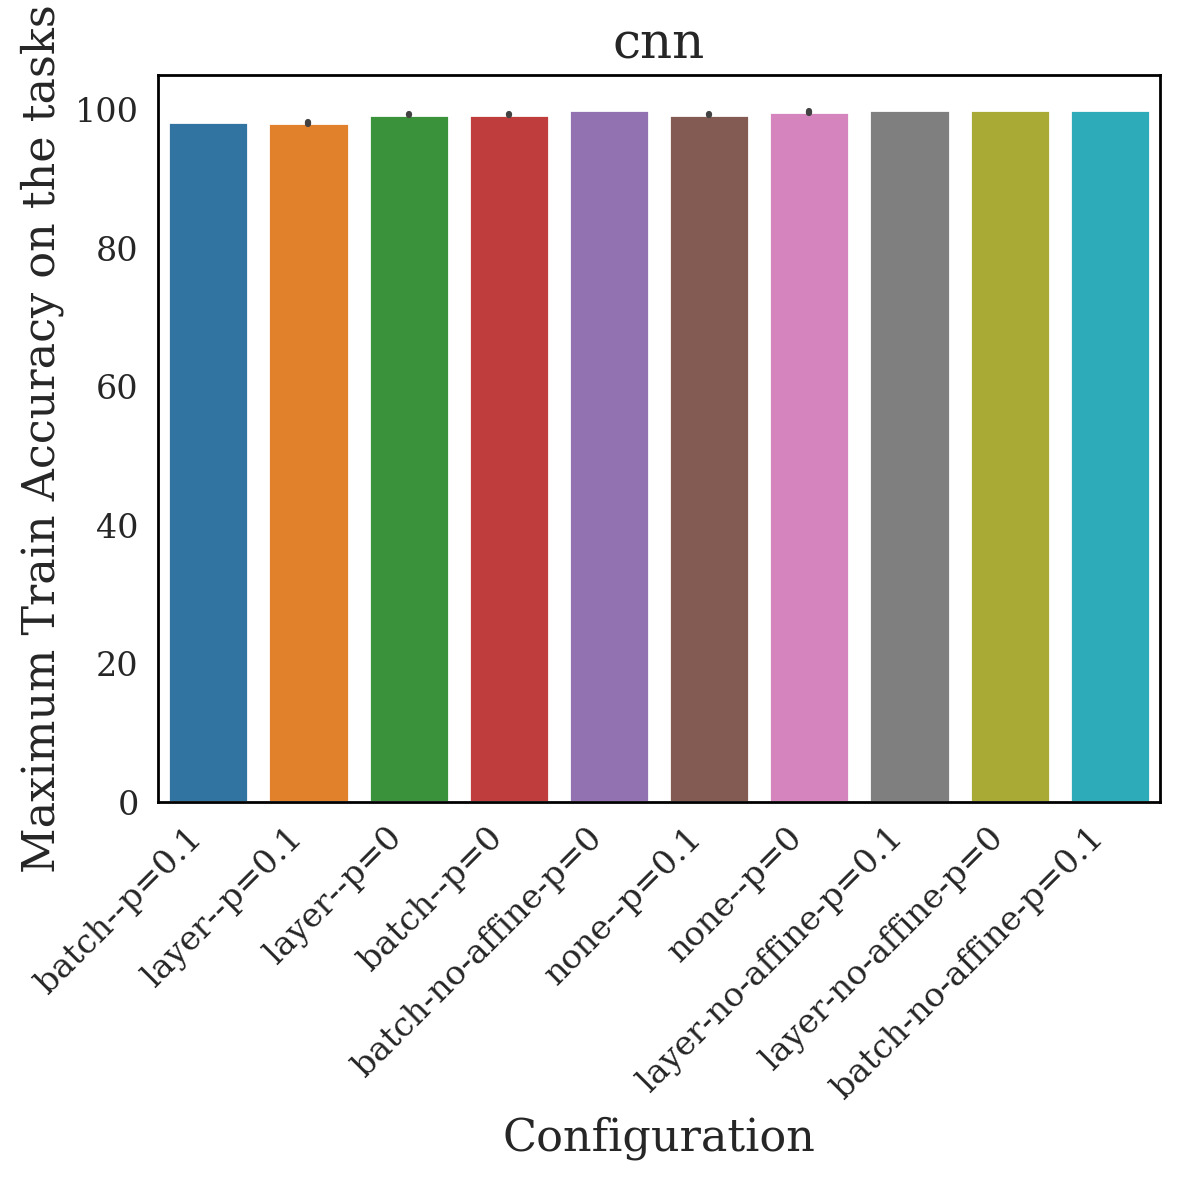
\includegraphics[width=0.3\linewidth]{cnn_config_finalperf.png}
    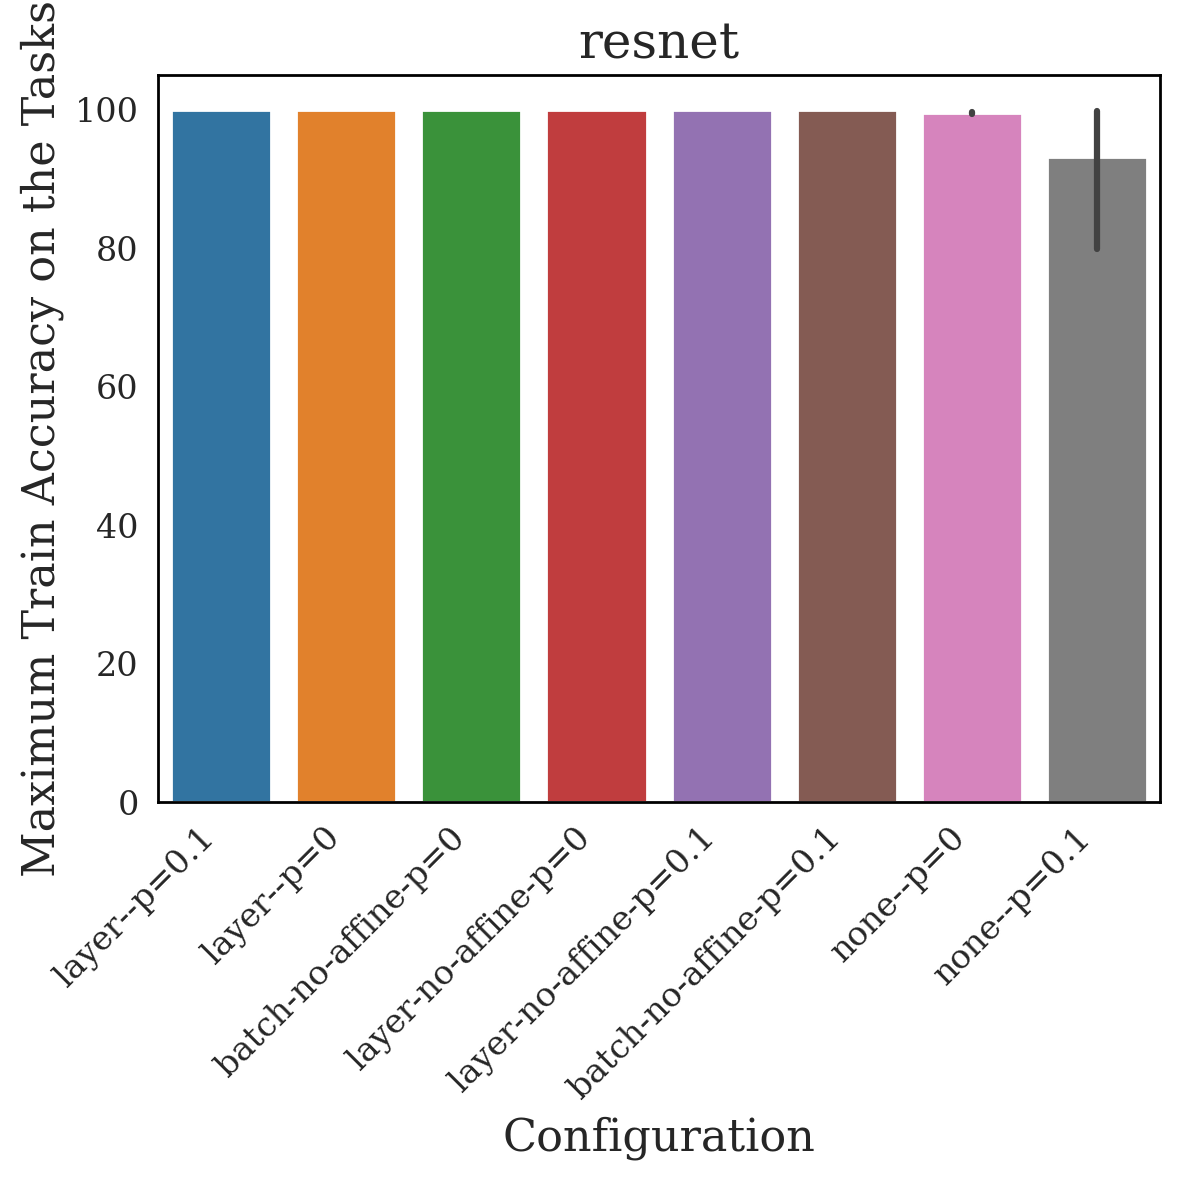
\includegraphics[width=0.3\linewidth]{resnet_config_finalperf.png}
    % 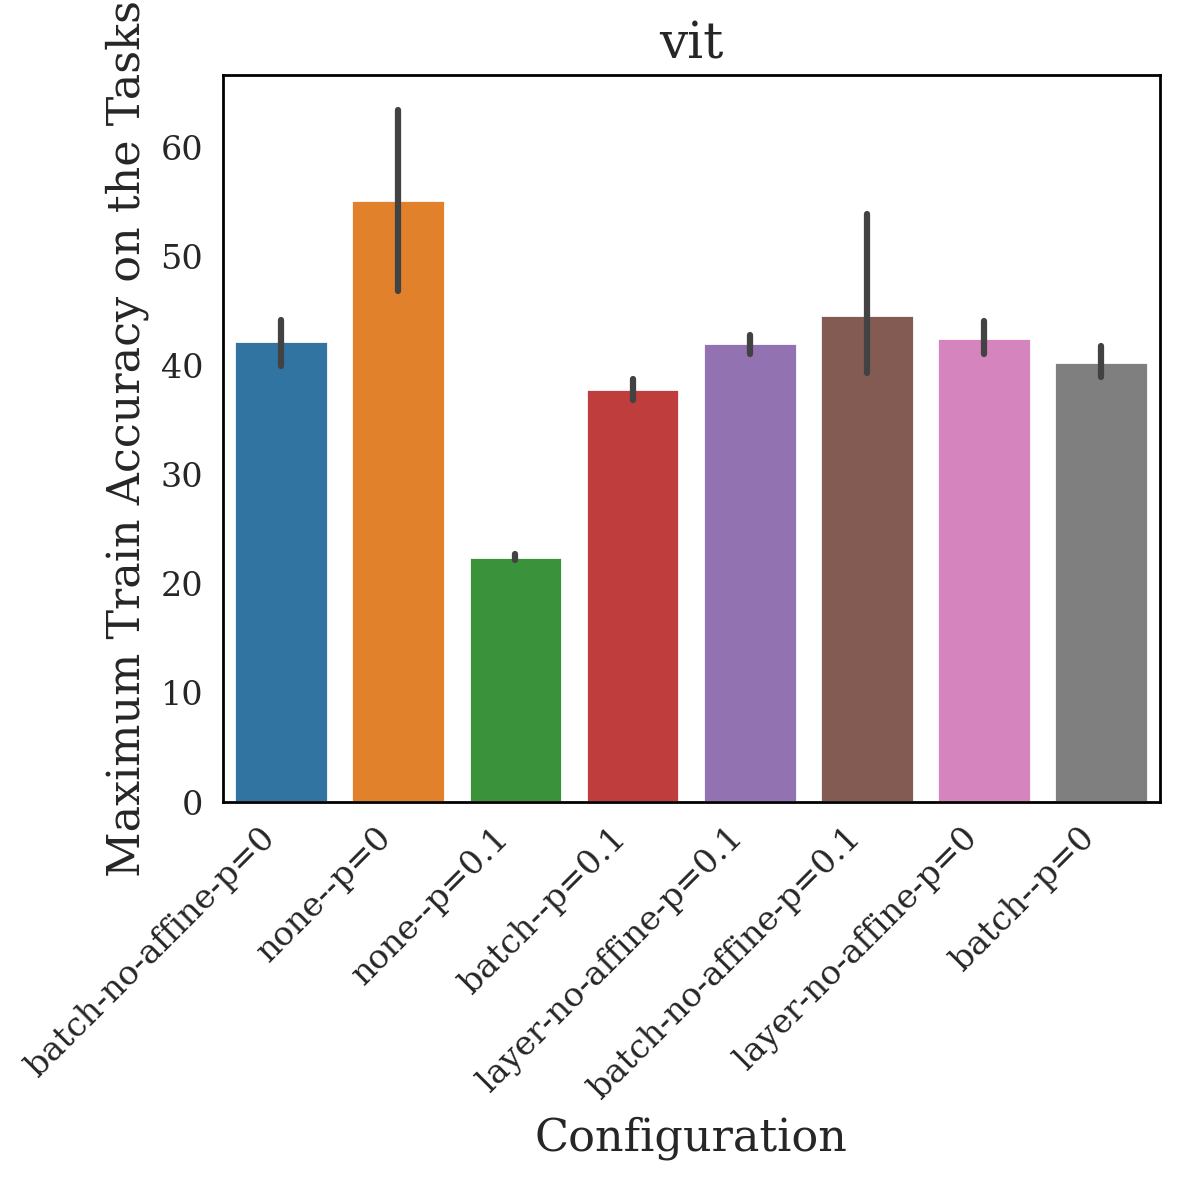
\includegraphics[width=0.33\linewidth]{vit_config_finalperf.png} % Included in user's draft, can be added if space allows
    \caption{(Placeholder figure/table) Summary of final performance (e.g., average max accuracy on continual tasks) for MLP, CNN, ResNet (and ViT) under different configurations of normalization and dropout. This highlights how architectural choices impact sustained learning capability.}
    \label{fig:mlp-config-finalperf}
\end{figure}

\section{Discussion and Open Questions}

This work introduces a mathematical framework using dynamical systems theory to analyze Loss of Plasticity (LoP) in deep neural networks. We formally define LoP manifolds as subspaces where gradient-based learning dynamics become trapped, leading to a diminished capacity for future adaptation. Our analysis identifies two primary mechanisms for such trapping: activation saturation leading to \emph{frozen units}, and representational redundancy resulting in \emph{cloned-unit manifolds}. These mechanisms provide a unifying lens through which to view various empirically observed phenomena associated with LoP, such as dead ReLU units \citep{nair2010rectified}, aspects of neural collapse related to representational degeneracy \citep{papyan2020prevalence}, and issues stemming from weight symmetry or duplication \citep{huh2022lowrank}.

A central theme emerging from our analysis is the fundamental tension between properties often considered beneficial for generalization in static learning environments and the demands of continual learning. Low-rank representations and simplicity biases, which can improve performance on fixed datasets \citep{huh2022lowrank, papyan2020prevalence, zhang2017understanding}, appear to be manifestations of the network settling into these lower-dimensional LoP manifolds. While such compression is advantageous for a single, static task, it inherently restricts the network's ability to learn new, potentially orthogonal information, thereby precipitating LoP in dynamic settings, as highlighted by \citet{dohare2024loss}.

This framework opens several avenues for future research:
\begin{itemize}[nosep]
    \item \textbf{Designing Effective Continual Randomization:} Given that initial randomness is a finite resource consumed during training, how can we develop \emph{ongoing} randomization strategies that effectively prevent parameter trajectories from being captured by stable LoP manifolds? While methods like Dropout \citep{srivastava2014dropout} and continual backpropagation \citep{dohare2024loss} offer partial solutions, more adaptive or targeted noise injection, possibly guided by online diagnostics of plasticity or manifold proximity, could be more effective.
    \item \textbf{Interaction with Advanced Optimizers:} How do optimization algorithms beyond first-order gradient descent, such as second-order methods utilizing Hessian information (relevant to Corollary~\ref{cor:perturb}'s curvature conditions), interact with LoP manifolds? Could these methods inherently detect and navigate away from or escape such stable regions? Furthermore, can meta-gradient approaches \citep{sutton1992gain} learn optimization strategies that explicitly maintain plasticity?
    \item \textbf{Characterizing Non-Linear Manifolds:} Our current analysis primarily focuses on mechanisms leading to affine or linear LoP subspaces (e.g., fixed parameters for frozen units, linear constraints for cloned units). Can LoP also arise from trapping in more complex, non-linear stable manifolds? Identifying and characterizing such manifolds would necessitate an extension of the current dynamical systems analysis.
    \item \textbf{Plasticity in Parameter-Efficient Fine-Tuning (PEFT):} PEFT methods like LoRA \citep{hu2021lora} and Adapters \citep{houlsby2019parameter} achieve efficiency by restricting updates to low-dimensional subspaces. Does this inherent low-dimensionality render PEFT methods particularly susceptible to a form of LoP where the adaptive subspace itself saturates or collapses during continual learning? Understanding and maintaining plasticity within these constrained frameworks is crucial for their application in lifelong learning scenarios.
    \item \textbf{LoP, Cloning, and Optimization Challenges:} This work reveals a connection between LoP in neural networks and the phenomenon of unit cloning. This link may offer new insights into broader challenges related to network optimization and redundancy. For instance, the conditions under which cloning occurs and its stability might inform the design of regularizers or optimizers that promote more diverse and efficient representations, potentially mitigating issues beyond just LoP, such as difficulties in escaping certain saddle points or achieving better generalization by avoiding overly redundant solutions. The role of noisy optimizers in potentially breaking cloning symmetries warrants further investigation.
\end{itemize}

Addressing these questions is pivotal for the development of AI systems capable of robust, lifelong learning and adaptation in the face of complex and evolving environments.

% \section{Broader Impacts} 
% This section was present in the template, and a draft was provided.
% It can be included if required by the venue.
% This research contributes to the fundamental understanding of limitations inherent in current deep learning paradigms, particularly concerning their ability to learn continuously and adapt over long time horizons. Positive societal impacts could arise from the development of more robust and adaptive AI systems. Systems capable of maintaining plasticity could adapt to changing conditions in the real world without significant performance degradation or the need for frequent, costly retraining from scratch. This could lead to more reliable autonomous systems (e.g., in robotics or vehicles), personalized learning systems that adapt to individual users over time, and AI that remains effective in dynamic environments like finance or climate modeling.
% However, potential negative impacts must also be considered. Enabling AI systems to adapt continually and indefinitely also raises concerns about predictability and control. If systems adapt in unforeseen ways or develop unexpected behaviors due to prolonged interaction with complex environments, it could lead to safety risks, especially in critical applications. Furthermore, understanding how to maintain plasticity might inadvertently lead to systems that are more difficult to audit or interpret, as their internal representations would be constantly shifting. The theoretical framework developed here provides tools not only for potentially enhancing plasticity but also for better understanding the conditions under which adaptation might become unstable or unpredictable, thereby contributing to the development of safer and more reliable continual learning systems. Responsible development and deployment, including robust testing and monitoring protocols, will be essential to mitigate these risks.


\bibliography{refs} % Assuming the bib file is named refs.bib

\appendix

\section{Proofs}
\label{app:proofs}

\begin{proof}[Proof Sketch for Proposition~\ref{prop:rank_recovery_nonlinearity} (Rank Recovery with Non-linearity)]
% This proof is based on the text provided for Prop 4.1 in the original draft's appendix
Let $f:\R\to\R$ be square-integrable w.r.t. $\gamma = \mathcal{N}(0,1)$ and not a polynomial. Let $z \sim \mathcal{N}(0, \Sigma)$ with $\Sigma_{ii}=1$ and $|\Sigma_{ij}| < 1$ for $i \neq j$. We want to show $C_{post} = \E[f(z)f(z)^\top]$ is full rank.
Since $f$ is square-integrable w.r.t. $\gamma$, it has a Hermite expansion $f(x) = \sum_{k=0}^{\infty} c_k \He_k(x)$, where $\He_k(x)$ are Hermite polynomials (scaled appropriately, e.g., probabilists' or physicists'). Since $f$ is not a polynomial, infinitely many $c_k$ must be non-zero.

The $(i, j)$-th entry of the covariance matrix $C_{post}$ is $C_{post, ij} = \E[f(z_i) f(z_j)]$. Substituting the Hermite expansion:
\begin{align*}
C_{post, ij} &= \E\left[ \left( \sum_{k=0}^{\infty} c_k \He_k(z_i) \right) \left( \sum_{l=0}^{\infty} c_l \He_l(z_j) \right) \right] \\
&= \sum_{k=0}^{\infty} \sum_{l=0}^{\infty} c_k c_l \E[\He_k(z_i) \He_l(z_j)]
\end{align*}
Using Mehler's formula for $\E[\He_k(Z_1) \He_l(Z_2)]$ where $(Z_1, Z_2)$ are jointly Gaussian with correlation $\rho = \Sigma_{ij}$ (and unit variance), $\E[\He_k(Z_i) \He_l(Z_j)] = \delta_{kl} k! (\Sigma_{ij})^k$ (using probabilists' Hermite polynomials, or $2^k k! (\Sigma_{ij})^k$ for physicists').
Thus,
$C_{post, ij} = \sum_{k=0}^{\infty} c_k^2 k! (\Sigma_{ij})^k = \sum_{k=0}^{\infty} a_k (\Sigma_{ij})^k$, where $a_k = c_k^2 k! \ge 0$.
The matrix $C_{post}$ can be written as $C_{post} = \sum_{k=0}^{\infty} a_k \Sigma^{\odot k}$, where $\Sigma^{\odot k}$ is the element-wise $k$-th power (Hadamard power) of $\Sigma$.
$\Sigma^{\odot 0}$ is a matrix of all ones. $\Sigma^{\odot 1} = \Sigma$.
Since $\Sigma$ is positive definite (as $|\Sigma_{ij}|<1$ for $i \ne j$ and $\Sigma_{ii}=1$ implies distinct, non-collinear variables), and the Hadamard product of positive definite matrices is positive definite (Schur product theorem), $\Sigma^{\odot k}$ is positive definite for $k \ge 1$.
Since infinitely many $c_k \neq 0$, infinitely many $a_k > 0$.
$C_{post}$ is a sum of positive semidefinite matrices $\Sigma^{\odot k}$ (for $k=0$) and positive definite matrices $\Sigma^{\odot k}$ (for $k \ge 1$ where $a_k > 0$). As long as at least one $a_k > 0$ for $k \ge 1$ (which is true if $f$ is not constant, which it isn't if it's non-linear), and $\Sigma$ corresponds to variables that are not all identical or perfectly collinear, $C_{post}$ will be positive definite, hence full rank. The condition $|\Sigma_{ij}| < 1$ ensures $\Sigma$ itself is positive definite if $d > 1$.
The argument for effective rank involving $c = \E[(f'(Z))^2]$ is more nuanced and often derived for weakly non-linear activations or specific assumptions about $\Sigma$ (e.g., near rank-one).
\end{proof}


\begin{proof}[Proof of Proposition~\ref{prop:cloned} (Cloned-unit plasticity loss)]
Let $\widetilde{G}=(\widetilde{V},\widetilde{E},\widetilde{W})$ be the cloned network and $G=(V,E,W)$ the base network, with surjection $\pi:\widetilde{V}\to V$ defining partitions $S_i:=\pi^{-1}(i)$. Assume identical activation functions $f_j$ for all $\widetilde{u} \in S_j$. The cloning conditions on initial weights $\widetilde{W}_0$ are as stated in Proposition~\ref{prop:cloned}.

\textbf{Base Case (Input Layer):} For input layer nodes, activations are determined by the input data $x$. If inputs are provided consistently with the cloning (e.g., all $\widetilde{u} \in S_i$ corresponding to an input node $i \in V_{in}$ receive the same input component $x_i$), then $h(\widetilde{u})$ is identical for all $\widetilde{u} \in S_i$.

\textbf{Inductive Step (Forward Pass - Activations):} Assume that for all partitions $S_k$ up to a certain depth, and for any $k \in V$, all nodes $\widetilde{u} \in S_k$ have identical activations, $h(\widetilde{u}) = h_k$.
Consider a node $\widetilde{v} \in S_j$ in the next layer. Its pre-activation $z(\widetilde{v})$ is:
$z(\widetilde{v}) = \sum_{i \in V \text{ s.t. } (i,j) \in E} \sum_{\widetilde{u} \in S_i, (\widetilde{u},\widetilde{v}) \in \widetilde{E}} \widetilde{w}_{\widetilde{u}\widetilde{v}} h(\widetilde{u})$.
By the induction hypothesis, $h(\widetilde{u}) = h_i$ for all $\widetilde{u} \in S_i$. So,
$z(\widetilde{v}) = \sum_{i \in V \text{ s.t. } (i,j) \in E} h_i \left( \sum_{\widetilde{u} \in S_i, (\widetilde{u},\widetilde{v}) \in \widetilde{E}} \widetilde{w}_{\widetilde{u}\widetilde{v}} \right)$.
By cloning condition (ii) of Proposition~\ref{prop:cloned}, $\sum_{\widetilde{u} \in S_i, (\widetilde{u},\widetilde{v}) \in \widetilde{E}} \widetilde{w}_{\widetilde{u}\widetilde{v}} = w_{ij}$ for any $\widetilde{v} \in S_j$.
Thus, $z(\widetilde{v}) = \sum_{i \in V \text{ s.t. } (i,j) \in E} h_i w_{ij}$. This value is independent of the choice of $\widetilde{v} \in S_j$; it is $z_j$, the pre-activation of node $j$ in the base network $G$.
Since $f_j$ is the activation function for all nodes in $S_j$, $h(\widetilde{v}) = f_j(z_j)$, which is also identical for all $\widetilde{v} \in S_j$.
By induction, all nodes within any partition $S_j$ have identical activations.

\textbf{Inductive Step (Backward Pass - Error Signals):} Assume that for all partitions $S_k$ down to a certain depth from the output, and for any $k \in V$, all nodes $\widetilde{u} \in S_k$ have identical error signals, $\delta(\widetilde{u}) = \delta_k$.
For output nodes $\widetilde{v} \in S_j$ where $j \in V_{out}$, $\delta(\widetilde{v}) = \partial\Loss/\partial h(\widetilde{v})$. Since $h(\widetilde{v})=h_j$ is identical for all $\widetilde{v} \in S_j$, and assuming the loss function treats these cloned outputs symmetrically, $\delta(\widetilde{v})$ will be identical, say $\delta_j$.
Now consider a hidden node $\widetilde{u} \in S_i$. Its error signal is:
$\delta(\widetilde{u}) = f'_i(z_i) \sum_{j \in V \text{ s.t. } (i,j) \in E} \sum_{\widetilde{v} \in S_j, (\widetilde{u},\widetilde{v}) \in \widetilde{E}} \delta(\widetilde{v}) \widetilde{w}_{\widetilde{u}\widetilde{v}}$.
We know $f'_i(z_i)$ is constant for all $\widetilde{u} \in S_i$ because $z_i$ is. By induction hypothesis, $\delta(\widetilde{v}) = \delta_j$ for all $\widetilde{v} \in S_j$. So,
$\delta(\widetilde{u}) = f'_i(z_i) \sum_{j \in V \text{ s.t. } (i,j) \in E} \delta_j \left( \sum_{\widetilde{v} \in S_j, (\widetilde{u},\widetilde{v}) \in \widetilde{E}} \widetilde{w}_{\widetilde{u}\widetilde{v}} \right)$.
By cloning condition (i) of Proposition~\ref{prop:cloned}, $\sum_{\widetilde{v} \in S_j, (\widetilde{u},\widetilde{v}) \in \widetilde{E}} \widetilde{w}_{\widetilde{u}\widetilde{v}} = w_{ij}$ for any $\widetilde{u} \in S_i$.
Thus, $\delta(\widetilde{u}) = f'_i(z_i) \sum_{j \in V \text{ s.t. } (i,j) \in E} \delta_j w_{ij}$. This value is independent of the choice of $\widetilde{u} \in S_i$; it is $\delta_i$, the error signal of node $i$ in the base network.
By induction, all nodes within any partition $S_i$ have identical error signals.

\textbf{Gradient Symmetry and Manifold Confinement:}
The gradient for a weight $\widetilde{w}_{\widetilde{u}\widetilde{v}}$ where $\widetilde{u} \in S_i$ and $\widetilde{v} \in S_j$ is $\frac{\partial\Loss}{\partial \widetilde{w}_{\widetilde{u}\widetilde{v}}} = \delta(\widetilde{v}) f'_j(z_j) h(\widetilde{u})$.
Since $\delta(\widetilde{v})=\delta_j$, $f'_j(z_j)$ is constant, and $h(\widetilde{u})=h_i$, this gradient is $\delta_j f'_j(z_j) h_i$. This value is the same for all weights connecting partition $S_i$ to $S_j$. Let this gradient be $g_{ij}$.
Any gradient update $\Delta \widetilde{w}_{\widetilde{u}\widetilde{v}} = -\eta g_{ij}$ will be identical for all such weights.
If the initial weights $\widetilde{W}_0$ satisfy the cloning conditions (e.g., if they are block-wise constant in a way that satisfies the sum conditions, or more generally just satisfy the sum conditions), then $\widetilde{W}(t) = \widetilde{W}_0 - \eta \sum \nabla\Loss(\widetilde{W}(\tau))$ will maintain the property that the changes $\widetilde{W}(t) - \widetilde{W}_0$ are block-wise constant (or preserve the sum conditions).
The parameters $\widetilde{W}(t)$ are confined to an affine subspace defined by $\widetilde{W}_0$ plus changes that maintain the cloning structure. The effective number of independent parameters driving the dynamics is that of the base network $G$, i.e., $|E|$. This manifold is stable under first-order gradient descent because the gradients themselves possess the symmetry.
\end{proof}


\section{Synthetic Validation of Rank Recovery Principles}
\label{app:rank_validation_appendix_label} % Renamed from app:additional_empirical_evidence for clarity

This appendix provides synthetic validations for the discussion in Section~\ref{sec:feature_dynamics} and Section~\ref{sec:mitigate} concerning how activation functions and normalization interact to influence feature rank.

\begin{figure}[ht!]
    \centering
    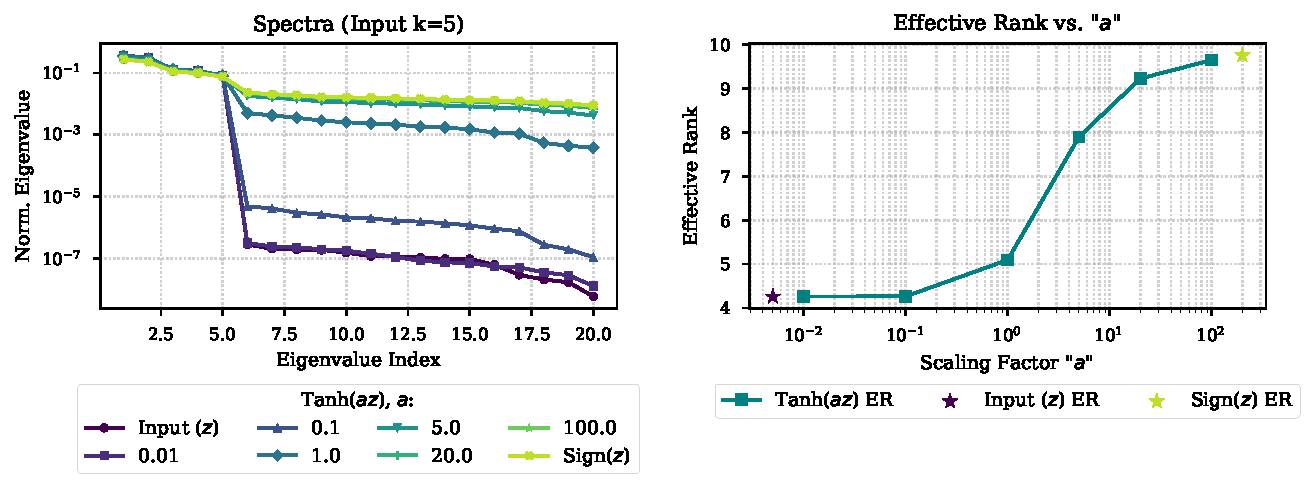
\includegraphics[width=0.7\linewidth]{theory_tanh_az_rank.pdf} 
    \caption{Effect of input scaling on post-activation effective rank for $h = \tanh(az)$, with rank-deficient pre-activations $z$ (initial Effective Rank (ER) $\approx 5$, full dimension $d_{\text{full}}=20$). \textbf{Left:} Normalized eigenvalue spectra of $\mathrm{Cov}(h)$. \textbf{Right:} Effective rank of $\mathrm{Cov}(h)$ vs. scaling factor $a$. Small $a$ makes $\tanh(az) \approx az$, leading to linear behavior and minimal rank increase. Appropriate intermediate $a$ values enhance non-linearity and maximize rank recovery. Very large $a$ makes $\tanh(az) \approx \mathrm{sign}(z)$, which also results in high rank features.}
    \label{fig:theory_tanh_az_rank}
\end{figure}

\begin{figure}[ht!]
    \centering
    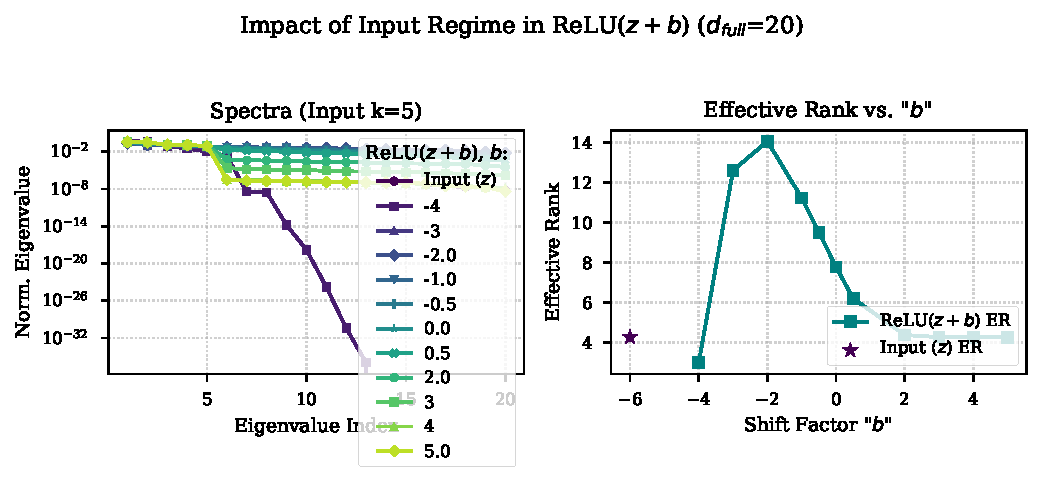
\includegraphics[width=0.7\linewidth]{theory_relu_zb_rank.pdf} 
    \caption{Effect of input shifting on post-activation effective rank for $h = \mathrm{ReLU}(z+b)$, with rank-deficient $z$ (initial ER $\approx 5$, $d_{\text{full}}=20$). \textbf{Left:} Normalized eigenvalue spectra of $\mathrm{Cov}(h)$. \textbf{Right:} Effective rank of $\mathrm{Cov}(h)$ vs. shift $b$. Large positive $b$ (making most $z_i+b > 0$) results in nearly affine behavior ($\mathrm{ReLU}(z+b) \approx z+b$ for positive inputs), limiting rank recovery. Large negative $b$ (making most $z_i+b < 0$) causes rank collapse as most outputs become zero. An optimal $b$ (typically near zero for zero-mean $z$) maximizes the non-linear effectiveness of ReLU around its kink, enhancing rank expansion.}
    \label{fig:theory_relu_zb_rank}
\end{figure}

Figures~\ref{fig:theory_tanh_az_rank} and \ref{fig:theory_relu_zb_rank} illustrate that the rank-expanding capability of non-linear activations like Tanh and ReLU is highly dependent on their input statistics. If inputs fall into regions where the activation is effectively linear (small inputs for Tanh, all-positive inputs for ReLU) or overly saturated, their capacity to increase representational rank is diminished. This underscores the importance of controlling pre-activation statistics, often achieved through normalization layers. Figure~\ref{fig:theory_joint_norm_activation_rank} demonstrates the synergistic effect of Batch Normalization (BN) in maintaining the effective non-linearity of activations.

\begin{figure}[ht!]
    \centering
    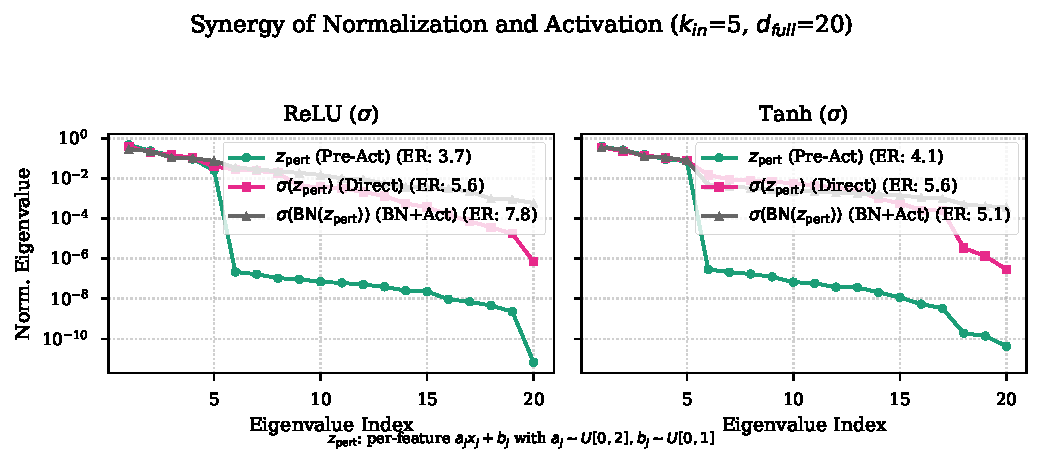
\includegraphics[width=0.7\linewidth]{theory_joint_norm_activation_rank.pdf} 
    \caption{Synergy of Batch Normalization (BN) with ReLU and Tanh for rank recovery from perturbed inputs $z_{\text{pert}}$ (initial ER $\approx 5$, $d_{\text{full}}=20$, then subjected to per-feature random scaling/shifting to degrade statistics). Plots show normalized eigenvalue spectra for the covariance matrix of: (i) $z_{\text{pert}}$ itself (blue, 'Pre-Act'), (ii) activation applied directly to $z_{\text{pert}}$ (orange, 'Direct'), and (iii) activation applied to $\text{BN}(z_{\text{pert}})$ (green, 'BN+Act'). Applying BN before the activation (green curves) consistently restores or enhances the effective rank, counteracting the detrimental effects of poor input statistics and highlighting BN's role in maintaining effective non-linearity.}
    \label{fig:theory_joint_norm_activation_rank}
\end{figure}

The empirical results for a Multi-Layer Perceptron (MLP) trained on MNIST, presented in Figure~\ref{fig:empirical_all_metrics}, further illustrate these points in a practical deep learning context.

\begin{figure}[h!]
    \centering
    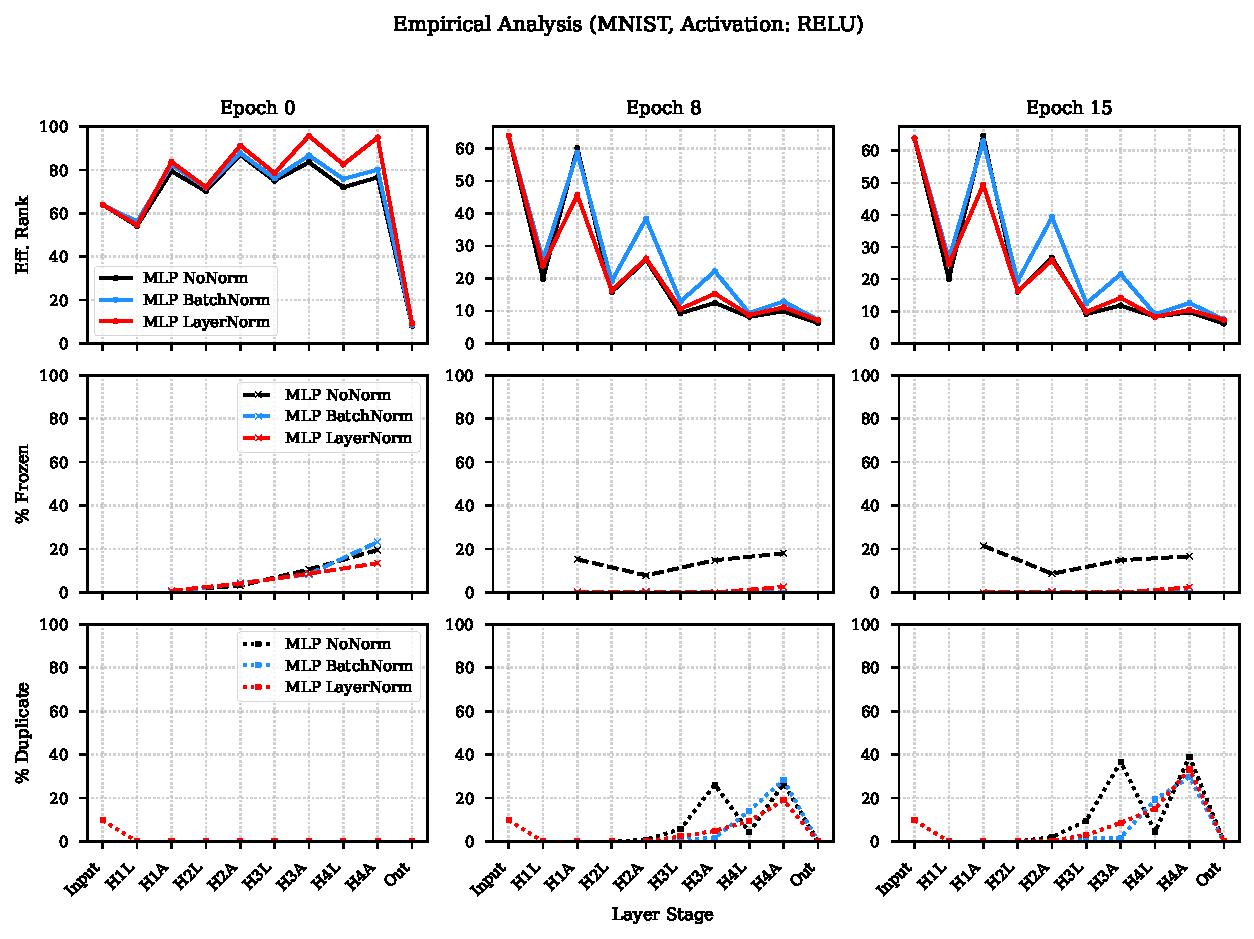
\includegraphics[width=\textwidth]{empirical_all_metrics_ReLU_MNIST.pdf}
    \caption{Comprehensive empirical metrics for an MLP with ReLU activation trained on MNIST, comparing configurations: no normalization, Batch Normalization, and Layer Normalization (colors distinguish configurations, see legend within plots if available, otherwise inferred from context). Metrics shown are: (Top Row) Effective Rank, (Middle Row) Percentage of Frozen (Dead) ReLU Units, and (Bottom Row) Percentage of Duplicate Units (highly correlated neurons). Each column of subplots typically represents a different training epoch (e.g., early, mid, and late training stages from left to right). Normalization, especially Batch Normalization, generally helps maintain higher effective rank (consistent with Figure~\ref{fig:empirical_rank_progression}), and also tends to reduce the percentage of frozen units and duplicate units, particularly in later epochs. This indicates healthier network dynamics and preserved potential for plasticity when activations operate in well-conditioned regimes.}
    \label{fig:empirical_all_metrics}
\end{figure}

The trends in Figure~\ref{fig:empirical_all_metrics} (effective rank, top row) align with Figure~\ref{fig:empirical_rank_progression}. Furthermore, normalization, particularly BN, correlates with lower percentages of frozen ReLUs (middle row) and duplicate units (bottom row) as training progresses. This suggests that by ensuring well-conditioned inputs to activations, normalization not only aids rank preservation but also mitigates other LoP symptoms like unit saturation and representational redundancy.


\section{Corollary on Architectural Extensions and Optimizer Robustness}
\label{app:arch_extensions}
The framework, particularly Proposition~\ref{prop:cloned} on cloned units, can be conceptually extended to cover common architectural components and optimizer variations:

\paragraph{Architectural Components:}
\begin{itemize}
    \item \textbf{Bias Terms:} Bias terms can be viewed as weights connected to a fixed input unit with activation 1. The cloning analysis applies if bias terms within a partition $S_j$ are identical initially and receive identical gradient updates (which they would if their upstream $\delta_j f'_j(z_j)$ signals are cloned).
    \item \textbf{Convolutional Neural Networks (CNNs):} Proposition~\ref{prop:cloned} can be adapted by considering entire channels (or feature maps) as the ``units'' being cloned. If multiple channels in a convolutional layer learn to compute identical feature maps due to symmetric initialization of their filters and subsequent identical updates, they form a cloned-channel manifold, reducing effective capacity.
    \item \textbf{Normalization Layers (LayerNorm, RMSNorm) and Softmax:} These layers involve interactions across multiple units/features. If the inputs to such a layer belong to partitions $\{S_i\}$ where activations within each partition are identical ($h_i$), the statistics for normalization (mean, variance) or the denominator for softmax can be computed based on these cloned activations. For LayerNorm, if input $h_k$ belongs to $S_j$ (so $h_k = h_j$), the mean $\mu = \frac{1}{N_{layer}}\sum_{j \in \text{layer}} |S_j| h_j$ and variance $\sigma^2 = \frac{1}{N_{layer}}\sum_{j \in \text{layer}} |S_j| (h_j - \mu)^2 - \mu^2$. The output $(h_j - \mu) / \sqrt{\sigma^2 + \epsilon}$ will also be cloned for all units originally in $S_j$. Similar reasoning applies to Softmax. If parameters feeding into these layers maintain cloning, the outputs will also be cloned, confining dynamics, though the LoP manifold definition might be more complex than a simple affine subspace. An ad-hoc low-dimensional equivalent model can often be formulated.
\end{itemize}

\paragraph{Optimizer Robustness:}
The cloning result (Proposition~\ref{prop:cloned}) is robust to common first-order optimization algorithm variations:
\begin{itemize}
    \item \textbf{Mini-batch SGD:} Since the cloning structure (identical gradients for cloned weights) holds for the gradient of each individual sample, the averaged gradient over a mini-batch will also exhibit the same block-wise constant structure across cloned partitions. Thus, mini-batch SGD does not break the symmetry.
    \item \textbf{Momentum / Adam:} Optimizers like SGD with Momentum or Adam maintain running averages of past gradients (first moment) and squared gradients (second moment). If the raw gradients $\nabla\Loss(\widetilde{W})$ possess the cloning structure at each step, then the first and second moment estimates will also inherit this structure (element-wise operations preserve the equality across cloned dimensions). Consequently, the parameter updates derived from these statistics will preserve the cloning symmetry, and the trajectory remains confined to the LoP manifold.
\end{itemize}
These extensions suggest that the core mechanisms of plasticity loss identified are relevant across a wide range of modern deep learning architectures and standard first-order optimizers.

\section{Experimental Setup Details (Illustrative)}
\label{app:exp_setup}
% This section is a placeholder as per the original draft.
% A full paper would detail datasets, model architectures, hyperparameters, continual learning protocols, etc.
% For instance:
% \subsection{Datasets}
% CIFAR-10, CIFAR-100, permuted MNIST, Split ImageNet, etc.
% \subsection{Models}
% MLPs (e.g., [784, N, N, 10]), CNNs (e.g., LeNet-style, small ResNets), ViTs (e.g., ViT-Tiny).
% \subsection{Metrics Implementation}
% - Effective Rank: Typically computed from singular values of activation matrices.
% - Dead/Saturated Units: Percentage of ReLUs with zero output across a batch, or Sigmoid/Tanh units with derivative below a threshold.
% - Duplicate Units: Correlation between neuron activations/weights, or R2 cloning metric as described in Section~\ref{sec:cloned_units}.
% \subsection{Continual Learning Setup}
% Task sequences, replay buffer size (if any), optimizer details (Adam, SGD, learning rates, etc.).

Placeholder for detailed experimental setup. The main text figures (e.g., Fig~\ref{fig:empirical_rank_progression}, Fig~\ref{fig:empirical_all_metrics}) are based on experiments with MLPs on MNIST, and other architectures are mentioned for figures like Fig~\ref{fig:DeadReLUs-LoP}, \ref{fig:dupfrac-LoP-emergence}. Specifics for these would be detailed here.

\section{Additional Experimental Evidence: Layer-wise Detail}
\label{app:additional_layer_detail}

\begin{figure}[h!]
    \centering
    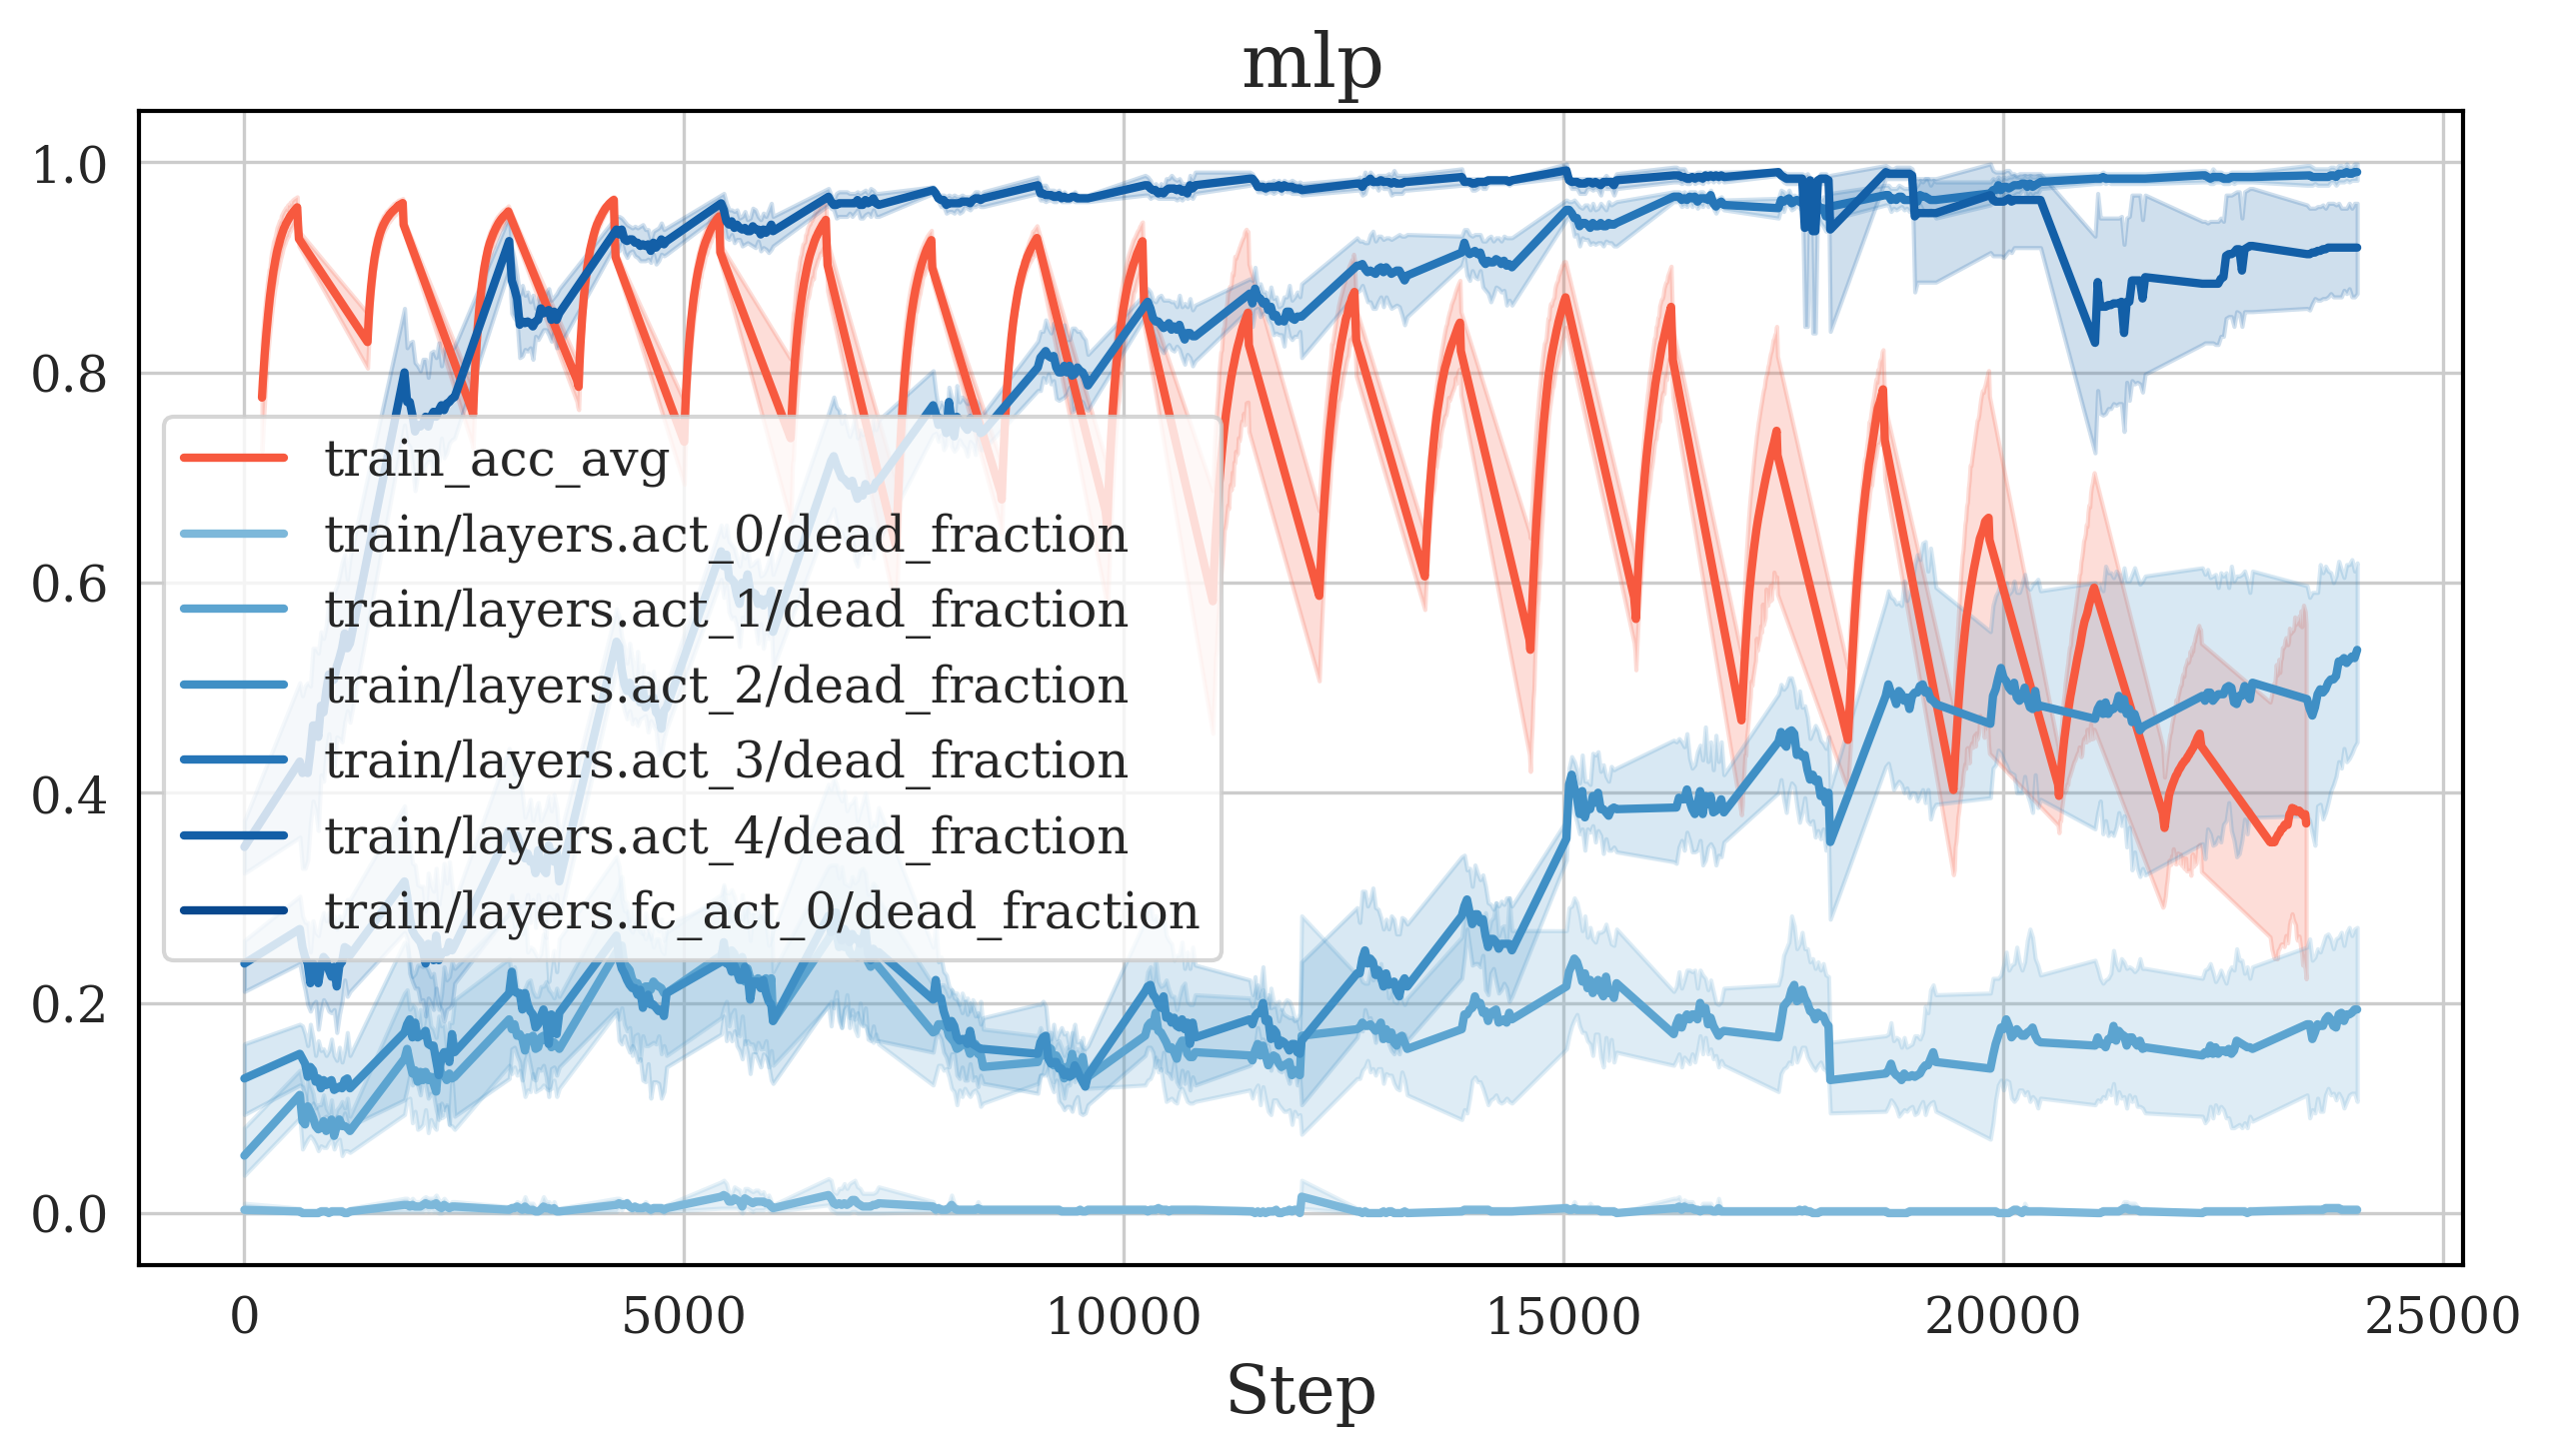
\includegraphics[width=0.45\linewidth]{dead_frac_mlp_layer_detail.png}
    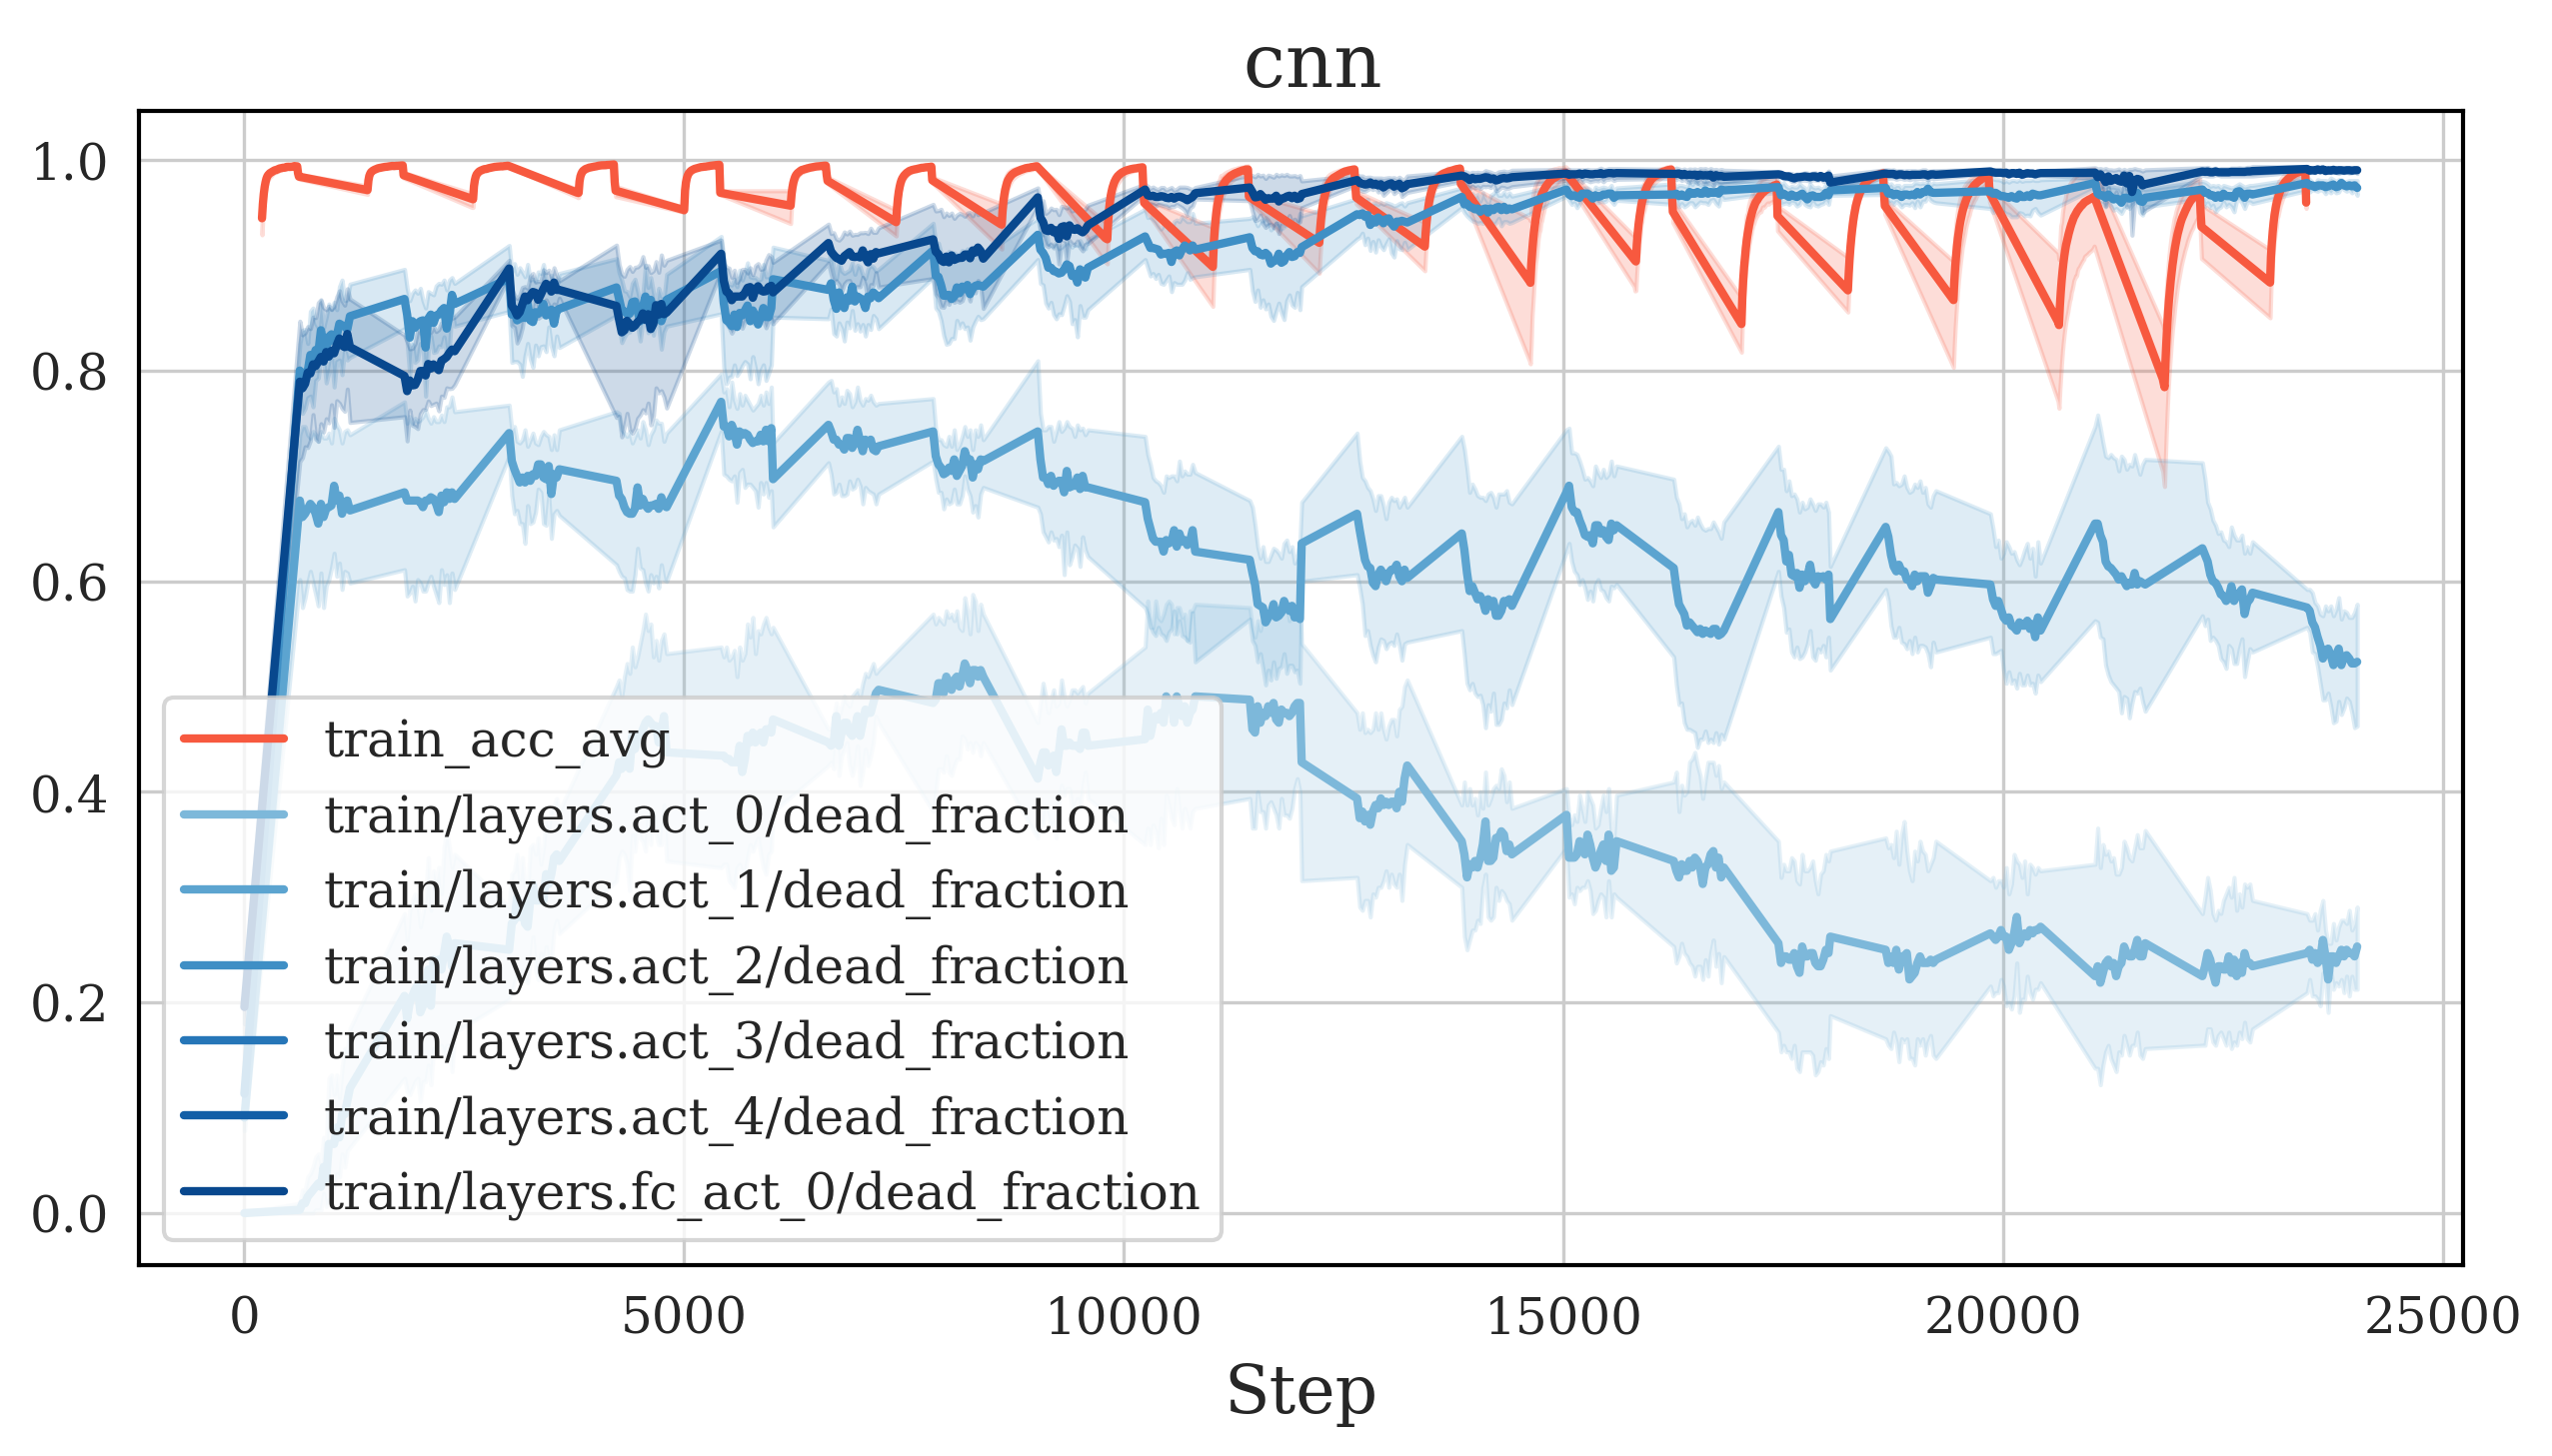
\includegraphics[width=0.45\linewidth]{dead_frac_cnn_layer_detail.png}
    \caption{(Placeholder figure) Layer-wise detail of dead unit fractions for MLP and CNN architectures, trained without normalization and dropout. Such plots can reveal if specific layers are more prone to unit saturation.}
    \label{fig:DeadReLUs-LayerDetail}
\end{figure}
\newpage

% NeurIPS Paper Checklist should be removed or updated for the specific submission version
% \section*{NeurIPS Paper Checklist}
% ... (Content from original draft) ...

\end{document}